\documentclass[a4paper,11pt,twoside]{article} 
%\documentclass{article}


\author{Victor LASSERRE \& Valentin SERVIERES}
\pdfminorversion=7 % To use charte graphique (pdf 1.7)
\usepackage[utf8]{inputenc}
\usepackage[T1]{fontenc}
\usepackage{lscape}
\usepackage{boldline,multirow,tabularx,colortbl,makecell,fancybox,amsfonts,amssymb,amsmath,mathrsfs,array, svg}
\usepackage{pgf,tikz,xcolor,graphicx}
\usetikzlibrary{calc,positioning,shapes.geometric,shapes.symbols,shapes.misc, fit, shapes, arrows, arrows.meta,fadings,through}
\usepackage[top=2cm, bottom=2cm, left=2cm, right=2cm]{geometry}
\usepackage{hyperref,titlesec,eurosym,eso-pic,float}
\usepackage[french]{babel}
%\usepackage{bibleref} ajouté par moi mais flemme
% minted et les encars de code en gros
%\usepackage[newfloat]{minted}
\usepackage{caption}
\usepackage{tcolorbox}
%\newenvironment{code}{\captionsetup{type=listing}}{}
%\SetupFloatingEnvironment{listing}{name=Code Source}

% table des annexes
\usepackage{minitoc}
\usepackage{pdfpages}

% bibliographie
%\usepackage{biblatex}
%\usepackage{csquotes}
%\addbibresource{bibliography.bib}

%%--------------------------------------------------------------%
%     This is the configuration file for package "listings"    %
%--------------------------------------------------------------%

%https://en.wikibooks.org/wiki/LaTeX/Source_Code_Listings

%\newcommand{\includecode}[2][c]{\lstinputlisting[language = #1, basicstyle=\ttfamily\bfseries]{#2}<!---->}


\definecolor{cgreen}{rgb}{0.596,0.765,0.475}
\definecolor{cgray}{rgb}{0.361,0.388,0.439}
\definecolor{cpurple}{rgb}{0.776,0.51,0.866}
\definecolor{cyellow}{rgb}{0.58,0,0.82}

\lstset{ 
  backgroundcolor = \color{white},   % choose the background color; you must add \usepackage{color} or \usepackage{xcolor}; should come as last argument
  basicstyle = \footnotesize,        % the size of the fonts that are used for the code
  breakatwhitespace = false,         % sets if automatic breaks should only happen at whitespace
  breaklines = true,                 % sets automatic line breaking
  captionpos = b,                    % sets the caption-position to bottom
  commentstyle = \color{cgray},      % comment style
  deletekeywords = {...},            % if you want to delete keywords from the given language
  escapeinside = {\%*}{*)},          % if you want to add LaTeX within your code
  extendedchars = true,              % lets you use non-ASCII characters; for 8-bits encodings only, does not work with UTF-8
  frame = single,	                   % adds a frame around the code
  keepspaces = true,                 % keeps spaces in text, useful for keeping indentation of code (possibly needs columns = flexible)
  keywordstyle = \color{blue},       % keyword style
  language = C,                     % the language of the code
  morekeywords = {*,...},            % if you want to add more keywords to the set
  numbers = left,                    % where to put the line-numbers; possible values are (none, left, right)
  numbersep = 5pt,                   % how far the line-numbers are from the code
  numberstyle = \tiny\color{black}, % the style that is used for the line-numbers
  rulecolor = \color{black},         % if not set, the frame-color may be changed on line-breaks within not-black text (e.g. comments (green here))
  showspaces = false,                % show spaces everywhere adding particular underscores; it overrides 'showstringspaces'
  showstringspaces = false,          % underline spaces within strings only
  showtabs = false,                  % show tabs within strings adding particular underscores
  stepnumber = 1,                    % the step between two line-numbers. If it's 1, each line will be numbered
  stringstyle = \color{cgreen},     % string literal style
  tabsize = 4,	                   % sets default tabsize to 2 spaces
  title = \lstname                   % show the filename of files included with \lstinputlisting; also try caption instead of title
}


\lstset{literate=
  {á}{{\'a}}1 {é}{{\'e}}1 {í}{{\'i}}1 {ó}{{\'o}}1 {ú}{{\'u}}1
  {Á}{{\'A}}1 {É}{{\'E}}1 {Í}{{\'I}}1 {Ó}{{\'O}}1 {Ú}{{\'U}}1
  {à}{{\`a}}1 {è}{{\`e}}1 {ì}{{\`i}}1 {ò}{{\`o}}1 {ù}{{\`u}}1
  {À}{{\`A}}1 {È}{{\'E}}1 {Ì}{{\`I}}1 {Ò}{{\`O}}1 {Ù}{{\`U}}1
  {ä}{{\"a}}1 {ë}{{\"e}}1 {ï}{{\"i}}1 {ö}{{\"o}}1 {ü}{{\"u}}1
  {Ä}{{\"A}}1 {Ë}{{\"E}}1 {Ï}{{\"I}}1 {Ö}{{\"O}}1 {Ü}{{\"U}}1
  {â}{{\^a}}1 {ê}{{\^e}}1 {î}{{\^i}}1 {ô}{{\^o}}1 {û}{{\^u}}1
  {Â}{{\^A}}1 {Ê}{{\^E}}1 {Î}{{\^I}}1 {Ô}{{\^O}}1 {Û}{{\^U}}1
  {œ}{{\oe}}1 {Œ}{{\OE}}1 {æ}{{\ae}}1 {Æ}{{\AE}}1 {ß}{{\ss}}1
  {ű}{{\H{u}}}1 {Ű}{{\H{U}}}1 {ő}{{\H{o}}}1 {Ő}{{\H{O}}}1
  {ç}{{\c c}}1 {Ç}{{\c C}}1 {ø}{{\o}}1 {å}{{\r a}}1 {Å}{{\r A}}1
  {€}{{\euro}}1 {£}{{\pounds}}1 {«}{{\guillemotleft}}1
  {»}{{\guillemotright}}1 {ñ}{{\~n}}1 {Ñ}{{\~N}}1 {¿}{{?`}}1
}

\tikzset{every picture/.style={execute at begin picture={
   \shorthandoff{:;!?};}
}}

\tikzset{
    boxnode/.style={ % requires library shapes.misc
        draw,
        rectangle,
        text centered,
        align=center,
        fill=gray!5!white
    },
}
\newcommand\tab[1][0.6cm]{\hspace*{#1}} %Create and define tab

\definecolor{lightgray}{gray}{0.85}
\definecolor{lightgrey}{gray}{0.85}
\definecolor{vlg}{gray}{0.85}


%Patch pour utiliser des équations dans les titres sans que hypperref nous insulte.
% Définition cyclique, compile pas. Mais c'est l"idée
%\renewcommand{\chapter}[1]{\chapter{\texorpdfstring{#1}}}
%\renewcommand{\section}[1]{\section{\texorpdfstring{#1}}}
%\renewcommand{\subsection}[1]{\subsection{\texorpdfstring{#1}}}
%\renewcommand{\subsubsection}[1]{\subsubsection{\texorpdfstring{#1}}}

%Chapter No Numbering but appears in TOC
\newcommand{\chapternn}[1]{\chapter*{#1}\addcontentsline{toc}{chapter}{#1}}
\newcommand{\sectionnn}[1]{\phantomsection\section*{#1}\addcontentsline{toc}{section}{#1}}
% phantomsection is necessary for links in TOC to function. It places the anchor
\newcommand{\subsectionnn}[1]{\subsection*{#1}\addcontentsline{toc}{subsection}{#1}}
\newcommand{\subsubsectionnn}[1]{\subsubsection*{#1}\addcontentsline{toc}{subsubsection}{#1}}

\newcolumntype{L}[1]{>{\raggedright\arraybackslash\hspace{0pt}}p{#1}}
\newcolumntype{R}[1]{>{\raggedleft\arraybackslash\hspace{0pt}}p{#1}}
\newcolumntype{C}[1]{>{\centering\arraybackslash\hspace{0pt}}p{#1}}


\renewcommand\thesection{\arabic{section}}
\renewcommand\thesubsection{\thesection.\arabic{subsection}}

%------- Do not append new commands after :

\hypersetup{	
    colorlinks=false, % colorise les liens
    linkbordercolor={1 1 1},
    breaklinks=true, % permet le retour à la ligne dans les liens trop longs
    urlcolor=blue, % couleur des hyperliens 
    linkcolor=black,	% couleur des liens internes 
    citecolor=black,	% couleur des références 
    pdftitle={}, % informations apparaissant dans 
    pdfauthor={}, % les informations du document
    pdfsubject={}	% sous Acrobat. 
}
\AtBeginDocument{\input{charteINSA/main_variables}
%\includepdf[pages={1}, scale=1.00]{charte_graphique.pdf}
\pagenumbering{gobble}
\thispagestyle{empty}
\definecolor{insa_blue}{RGB}{52,83,111}
\definecolor{insa_red}{RGB}{230,39,20}
\noindent\begin{tikzpicture}[remember picture, overlay, shift={(current page.south west)}]
    \draw[draw=none, fill=insa_red] (12.32,1.24) -- (12.32,4.94) -- (19.7,4.94) -- (19.7,1.24) -- cycle;
    \node[anchor=north west, align=left, text width=10cm] at (2.0,23.5) {\color{white} \varmaintitle};
    \node[anchor=north west, align=right, text width=8cm] at (-0.7,22.5) {\color{white} \varmainsubtitle};
    \node[anchor=north west] at (2,21.5) {\includegraphics[scale=0.25]{\varlogo}};
    \node[anchor=north west, align=left, text width=12cm] at (2.1,16) {\color{white} \varcovertext}; %-3, 4.1
    %\node[anchor=center, align=center, text width=12cm] at (10,6.7) {\color{black} \varcovertext}; %-3, 4.1
    \node[anchor=north west, align=left, text width=12cm] at (1.2,4.7) {\varinsaaddress};
    \node[anchor=north west, align=left, text width=12cm] at (12.5,4.7) {\color{white} \varcompanyaddress};
    \node[anchor=north west, align=left, text width=12cm] at (0.5,4) {\includepdf[pages={1}]{charteINSA/cover/charte_graphique}};
\end{tikzpicture}
\newpage 
\input{charteINSA/main_variables}
%\includepdf[pages={1}, scale=1.00]{charte_graphique.pdf}
\pagenumbering{gobble}
\thispagestyle{empty}
\definecolor{insa_blue}{RGB}{52,83,111}
\definecolor{insa_red}{RGB}{230,39,20}
\noindent\begin{tikzpicture}[remember picture, overlay, shift={(current page.south west)}]
    %\draw[draw=none, fill=insa_red] (12.32,1.24) -- (12.32,4.94) -- (19.7,4.94) -- (19.7,1.24) -- cycle;
    \node[anchor=north west, align=left, text width=10cm] at (2.0,23.5) {\color{black} \varmaintitle};
    \node[anchor=north west, align=right, text width=8cm] at (-0.7,22.5) {\color{black} \varmainsubtitle};
    %\node[anchor=north west] at (2,21.5) {\includegraphics[scale=0.09]{\varlogo}};
    \node[anchor=north west, align=left, text width=12cm] at (2.1,16) {\color{black} \varcovertext}; %-3, 4.1
    \node[anchor=north west, align=left, text width=12cm] at (1.2,4.7) {\varinsaaddress};
    \node[anchor=north west, align=left, text width=12cm] at (12.5,4.7) {\color{black} \varcompanyaddress};
    \node[anchor=north west, align=left, text width=12cm] at (0.5,4) {\includepdf[pages={2}]{charteINSA/cover/charte_graphique}};
\end{tikzpicture}
\newpage 
\pagenumbering{arabic}}

%\AtEndDocument{\newpage
\pagenumbering{gobble}
\thispagestyle{empty}
\definecolor{insa_blue}{RGB}{52,83,111}
\definecolor{insa_red}{RGB}{226,50,46}
\noindent\begin{tikzpicture}[remember picture, overlay, shift={(current page.south west)}]
    % \draw[draw=none, path fading=east, left color=insa_blue, right color=insa_blue!25!white] (21,7.3) -- (4.3,16.05) -- (21,24.8) -- cycle;
    % \draw[draw=none, path fading=east, left color=insa_blue, right color=insa_blue!60!white] (0,16.2) -- (7,19.75) -- (0,23.1) -- cycle;
    % \draw[draw=none, path fading=east, left color=insa_blue, right color=insa_blue!25!white] (0,17.3) -- (13.7,24.5) -- (2.3,29.7) -- (0,29.7) -- cycle;
    % 
    % 
    % \draw[draw=none, fill=insa_red] (6.2,0) -- (6.2,1.2) -- (11.6,0) -- cycle;
    % 
    % \draw[draw=none, fill=white] (0,0) -- (0,10) -- (10,10) -- (10,0) -- cycle;
    % \node[anchor=south west, align=left] at (1.25,3.6) {\textbf{INSA Toulouse}};
    % \node[anchor=south west, align=left] at (1.25,2.20) {135, Avenue de Rangueil \\ 31077 Toulouse Cedex 4 - France \\ \href{http://www.insa-toulouse.fr}{www.insa-toulouse.fr}};
    % 
    % \node[anchor=south west] at (11.1,2.2) {
\includegraphics[height=1cm, keepaspectratio]{----cover/meta/univ.png}};
    %\node[anchor=south west] at (13.4,2.2) {
\includegraphics[height=1cm, keepaspectratio]{----cover/meta/ministere.png}};
    % \node[anchor=north west, align=left, text width=12cm] at (0.5,4) {\includepdf[pages={2}]{----cover/charte_graphique}};
\end{tikzpicture}
}




%\usepackage[french]{babel}

% resolve no citation problem
%\nocite{*}
%\usepackage[...,backend=bibtex]{biblatex}

% Set page size and margins
% Replace `letterpaper' with `a4paper' for UK/EU standard size
%%%%%\usepackage[letterpaper,top=2cm,bottom=2cm,left=3cm,right=3cm,marginparwidth=1.75cm]{geometry}

% Useful packages
\usepackage{listings}

\input{preferences/listings-glsl.prf}
% optionally set GLSL as default language
\lstset{language=GLSL}
\lstset{
  breaklines=true,
  breakatwhitespace=true,
  numbers=left,
  basicstyle={\small\ttfamily},
  numberstyle=\tiny\color{gray},
  tabsize=3,% end normal settings
  breaklines=true,                              % break long lines
  commentstyle=\itshape\color{green},           % comments are green
  keywordstyle=[1]\color{blue},                 % instructions are blue
  keywordstyle=[2]\color{orange},               % sections/other directives are orange
  keywordstyle=[3]\color{red},                   % registers are red
  stringstyle=\color{mauve},                    % strings are from the telekom
  identifierstyle=\color{teal},                 % user declared addresses are teal
  frame=l,                                      % black line on the left side of code
  language=GLSL,                   % all code is RISC-V
  tabsize=4,                                    % indent tabs with 4 spaces
  showstringspaces=false                        % do not replace spaces with weird underlines
}


\usepackage{setspace}
\usepackage{titletoc}
%\usepackage[T1]{fontenc}
%\usepackage{amsfonts}
%\usepackage{graphicx}
\usepackage{mathtools}
\graphicspath{ {images/} }

%\usepackage{fancyhdr}
\pagestyle{fancy}
\renewcommand\headrulewidth{1pt}
\fancyhead[L]{\textsf{Moteur graphique}}
\fancyhead[R]{\textsf{}}
%\usepackage[colorlinks=true, allcolors=blue]{hyperref}


\begin{document}
%\maketitle
\cleardoublepage


% Remerciements
\thispagestyle{empty} % removes page number
\subsection*{Remerciements}
Avant de commencer ce rapport, nous tenions à remercier M. Sanchez, notre encadrant dans le cadre de ce projet.
\clearpage

% TABLE DES MATIÈRES
\thispagestyle{empty} % removes page number
\setcounter{secnumdepth}{3}
\tableofcontents
\clearpage

\setcounter{page}{1}


\sectionnn{Introduction}

    Engin Pas Tangible est un moteur graphique reposant sur le principe de Ray Marching : un système de 3D similaire au Ray Tracing, mais beaucoup plus rarement utilisé. Ce système a certains avantages par rapport au Ray Tracing, comme par exemple de permettre une implémetation peu coûteuse de fractales, ou autres figures se reproduisant à l'identique. \\
    Le Ray Marching repose sur la projection de rayons depuis une camera vers la scene. Pour projeter un rayon, on le fait avancer pas à pas (\emph{Marching}). La distance des pas doit être la plus grande possible, mais sans que le rayon ne traverse d'objet de la scene 3D.
\\
\\
%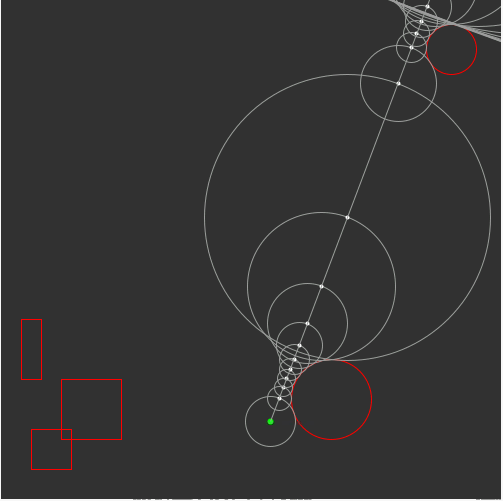
\includegraphics[width=8cm]{images/marching.png}
\begin{figure}[h]
    \centering
    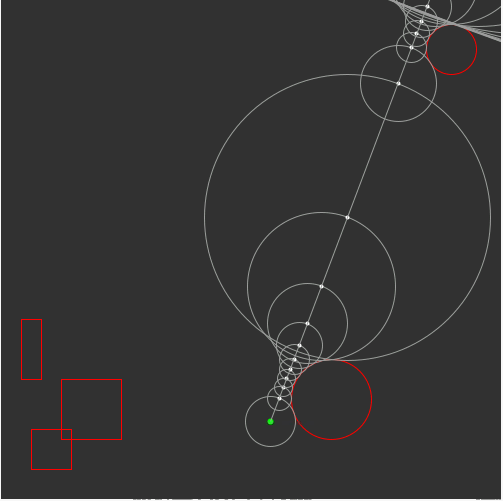
\includegraphics[width=8cm]{images/marching.png}
    \caption{Illustration 2D de la marche point par point d'un rayon (plus de details dans \ref{subsec:projection} \nameref{subsec:projection})}
    \label{fig:my_label}
\end{figure}

\clearpage
\documentclass[a4paper,11pt,twoside]{article} 
%\documentclass{article}


\author{Victor LASSERRE \& Valentin SERVIERES}
\pdfminorversion=7 % To use charte graphique (pdf 1.7)
\usepackage[utf8]{inputenc}
\usepackage[T1]{fontenc}
\usepackage{lscape}
\usepackage{boldline,multirow,tabularx,colortbl,makecell,fancybox,amsfonts,amssymb,amsmath,mathrsfs,array, svg}
\usepackage{pgf,tikz,xcolor,graphicx}
\usetikzlibrary{calc,positioning,shapes.geometric,shapes.symbols,shapes.misc, fit, shapes, arrows, arrows.meta,fadings,through}
\usepackage[top=2cm, bottom=2cm, left=2cm, right=2cm]{geometry}
\usepackage{hyperref,titlesec,eurosym,eso-pic,float}
\usepackage[french]{babel}
%\usepackage{bibleref} ajouté par moi mais flemme
% minted et les encars de code en gros
%\usepackage[newfloat]{minted}
\usepackage{caption}
\usepackage{tcolorbox}
%\newenvironment{code}{\captionsetup{type=listing}}{}
%\SetupFloatingEnvironment{listing}{name=Code Source}

% table des annexes
\usepackage{minitoc}
\usepackage{pdfpages}

% bibliographie
%\usepackage{biblatex}
%\usepackage{csquotes}
%\addbibresource{bibliography.bib}

%%--------------------------------------------------------------%
%     This is the configuration file for package "listings"    %
%--------------------------------------------------------------%

%https://en.wikibooks.org/wiki/LaTeX/Source_Code_Listings

%\newcommand{\includecode}[2][c]{\lstinputlisting[language = #1, basicstyle=\ttfamily\bfseries]{#2}<!---->}


\definecolor{cgreen}{rgb}{0.596,0.765,0.475}
\definecolor{cgray}{rgb}{0.361,0.388,0.439}
\definecolor{cpurple}{rgb}{0.776,0.51,0.866}
\definecolor{cyellow}{rgb}{0.58,0,0.82}

\lstset{ 
  backgroundcolor = \color{white},   % choose the background color; you must add \usepackage{color} or \usepackage{xcolor}; should come as last argument
  basicstyle = \footnotesize,        % the size of the fonts that are used for the code
  breakatwhitespace = false,         % sets if automatic breaks should only happen at whitespace
  breaklines = true,                 % sets automatic line breaking
  captionpos = b,                    % sets the caption-position to bottom
  commentstyle = \color{cgray},      % comment style
  deletekeywords = {...},            % if you want to delete keywords from the given language
  escapeinside = {\%*}{*)},          % if you want to add LaTeX within your code
  extendedchars = true,              % lets you use non-ASCII characters; for 8-bits encodings only, does not work with UTF-8
  frame = single,	                   % adds a frame around the code
  keepspaces = true,                 % keeps spaces in text, useful for keeping indentation of code (possibly needs columns = flexible)
  keywordstyle = \color{blue},       % keyword style
  language = C,                     % the language of the code
  morekeywords = {*,...},            % if you want to add more keywords to the set
  numbers = left,                    % where to put the line-numbers; possible values are (none, left, right)
  numbersep = 5pt,                   % how far the line-numbers are from the code
  numberstyle = \tiny\color{black}, % the style that is used for the line-numbers
  rulecolor = \color{black},         % if not set, the frame-color may be changed on line-breaks within not-black text (e.g. comments (green here))
  showspaces = false,                % show spaces everywhere adding particular underscores; it overrides 'showstringspaces'
  showstringspaces = false,          % underline spaces within strings only
  showtabs = false,                  % show tabs within strings adding particular underscores
  stepnumber = 1,                    % the step between two line-numbers. If it's 1, each line will be numbered
  stringstyle = \color{cgreen},     % string literal style
  tabsize = 4,	                   % sets default tabsize to 2 spaces
  title = \lstname                   % show the filename of files included with \lstinputlisting; also try caption instead of title
}


\lstset{literate=
  {á}{{\'a}}1 {é}{{\'e}}1 {í}{{\'i}}1 {ó}{{\'o}}1 {ú}{{\'u}}1
  {Á}{{\'A}}1 {É}{{\'E}}1 {Í}{{\'I}}1 {Ó}{{\'O}}1 {Ú}{{\'U}}1
  {à}{{\`a}}1 {è}{{\`e}}1 {ì}{{\`i}}1 {ò}{{\`o}}1 {ù}{{\`u}}1
  {À}{{\`A}}1 {È}{{\'E}}1 {Ì}{{\`I}}1 {Ò}{{\`O}}1 {Ù}{{\`U}}1
  {ä}{{\"a}}1 {ë}{{\"e}}1 {ï}{{\"i}}1 {ö}{{\"o}}1 {ü}{{\"u}}1
  {Ä}{{\"A}}1 {Ë}{{\"E}}1 {Ï}{{\"I}}1 {Ö}{{\"O}}1 {Ü}{{\"U}}1
  {â}{{\^a}}1 {ê}{{\^e}}1 {î}{{\^i}}1 {ô}{{\^o}}1 {û}{{\^u}}1
  {Â}{{\^A}}1 {Ê}{{\^E}}1 {Î}{{\^I}}1 {Ô}{{\^O}}1 {Û}{{\^U}}1
  {œ}{{\oe}}1 {Œ}{{\OE}}1 {æ}{{\ae}}1 {Æ}{{\AE}}1 {ß}{{\ss}}1
  {ű}{{\H{u}}}1 {Ű}{{\H{U}}}1 {ő}{{\H{o}}}1 {Ő}{{\H{O}}}1
  {ç}{{\c c}}1 {Ç}{{\c C}}1 {ø}{{\o}}1 {å}{{\r a}}1 {Å}{{\r A}}1
  {€}{{\euro}}1 {£}{{\pounds}}1 {«}{{\guillemotleft}}1
  {»}{{\guillemotright}}1 {ñ}{{\~n}}1 {Ñ}{{\~N}}1 {¿}{{?`}}1
}

\tikzset{every picture/.style={execute at begin picture={
   \shorthandoff{:;!?};}
}}

\tikzset{
    boxnode/.style={ % requires library shapes.misc
        draw,
        rectangle,
        text centered,
        align=center,
        fill=gray!5!white
    },
}
\newcommand\tab[1][0.6cm]{\hspace*{#1}} %Create and define tab

\definecolor{lightgray}{gray}{0.85}
\definecolor{lightgrey}{gray}{0.85}
\definecolor{vlg}{gray}{0.85}


%Patch pour utiliser des équations dans les titres sans que hypperref nous insulte.
% Définition cyclique, compile pas. Mais c'est l"idée
%\renewcommand{\chapter}[1]{\chapter{\texorpdfstring{#1}}}
%\renewcommand{\section}[1]{\section{\texorpdfstring{#1}}}
%\renewcommand{\subsection}[1]{\subsection{\texorpdfstring{#1}}}
%\renewcommand{\subsubsection}[1]{\subsubsection{\texorpdfstring{#1}}}

%Chapter No Numbering but appears in TOC
\newcommand{\chapternn}[1]{\chapter*{#1}\addcontentsline{toc}{chapter}{#1}}
\newcommand{\sectionnn}[1]{\phantomsection\section*{#1}\addcontentsline{toc}{section}{#1}}
% phantomsection is necessary for links in TOC to function. It places the anchor
\newcommand{\subsectionnn}[1]{\subsection*{#1}\addcontentsline{toc}{subsection}{#1}}
\newcommand{\subsubsectionnn}[1]{\subsubsection*{#1}\addcontentsline{toc}{subsubsection}{#1}}

\newcolumntype{L}[1]{>{\raggedright\arraybackslash\hspace{0pt}}p{#1}}
\newcolumntype{R}[1]{>{\raggedleft\arraybackslash\hspace{0pt}}p{#1}}
\newcolumntype{C}[1]{>{\centering\arraybackslash\hspace{0pt}}p{#1}}


\renewcommand\thesection{\arabic{section}}
\renewcommand\thesubsection{\thesection.\arabic{subsection}}

%------- Do not append new commands after :

\hypersetup{	
    colorlinks=false, % colorise les liens
    linkbordercolor={1 1 1},
    breaklinks=true, % permet le retour à la ligne dans les liens trop longs
    urlcolor=blue, % couleur des hyperliens 
    linkcolor=black,	% couleur des liens internes 
    citecolor=black,	% couleur des références 
    pdftitle={}, % informations apparaissant dans 
    pdfauthor={}, % les informations du document
    pdfsubject={}	% sous Acrobat. 
}
\AtBeginDocument{\input{charteINSA/cover/cover_in.tex}\input{charteINSA/cover/cover_in_2.tex}\pagenumbering{arabic}}

%\AtEndDocument{\input{----cover/cover_out.tex}}




%\usepackage[french]{babel}

% resolve no citation problem
\nocite{*}
%\usepackage[...,backend=bibtex]{biblatex}

% Set page size and margins
% Replace `letterpaper' with `a4paper' for UK/EU standard size
%%%%%\usepackage[letterpaper,top=2cm,bottom=2cm,left=3cm,right=3cm,marginparwidth=1.75cm]{geometry}

% Useful packages
\usepackage{listings}

\input{preferences/listings-glsl.prf}
% optionally set GLSL as default language
\lstset{language=GLSL}
\lstset{
  breaklines=true,
  breakatwhitespace=true,
  numbers=left,
  basicstyle={\small\ttfamily},
  numberstyle=\tiny\color{gray},
  tabsize=3,% end normal settings
  breaklines=true,                              % break long lines
  commentstyle=\itshape\color{green},           % comments are green
  keywordstyle=[1]\color{blue},                 % instructions are blue
  keywordstyle=[2]\color{orange},               % sections/other directives are orange
  keywordstyle=[3]\color{red},                   % registers are red
  stringstyle=\color{mauve},                    % strings are from the telekom
  identifierstyle=\color{teal},                 % user declared addresses are teal
  frame=l,                                      % black line on the left side of code
  language=GLSL,                   % all code is RISC-V
  tabsize=4,                                    % indent tabs with 4 spaces
  showstringspaces=false                        % do not replace spaces with weird underlines
}

\usepackage[square,numbers]{natbib}
\bibliographystyle{abbrvnat}
%Includes "References" in the table of contents
\usepackage[nottoc]{tocbibind}

\usepackage{setspace}
\usepackage{titletoc}
%\usepackage[T1]{fontenc}
%\usepackage{amsfonts}
%\usepackage{graphicx}
\usepackage{mathtools}
\graphicspath{ {images/} }

%\usepackage{fancyhdr}
\pagestyle{fancy}
\renewcommand\headrulewidth{1pt}
\fancyhead[L]{\textsf{Moteur graphique}}
\fancyhead[R]{\textsf{}}
%\usepackage[colorlinks=true, allcolors=blue]{hyperref}


\begin{document}
\dosecttoc{} % generate TOC
%\maketitle
\clearpage

% Remerciements
\thispagestyle{empty} % removes page number
\subsection*{Remerciements}
Nous tenons à remercier notre tuteur de projet M. Sanchez, notamment pour son aide précieuse et ses conseils. \\
Nous remercions également Inigo Quilez pour la riche documentation sur le ray marching qu'il fournit librement sur son site web.
\clearpage

% TABLE DES MATIÈRES
\thispagestyle{empty} % removes page number
\setcounter{secnumdepth}{3}
\tableofcontents
\clearpage

\setcounter{page}{1}


\sectionnn{Introduction}

    Engin Pas Tangible est un moteur graphique reposant sur le principe de Ray Marching : un système de 3D similaire au Ray Tracing, mais beaucoup plus rarement utilisé. Ce système a certains avantages par rapport au Ray Tracing, comme par exemple de permettre une implémetation peu coûteuse de fractales, ou autres figures se reproduisant à l'identique. \\
    Le Ray Marching repose sur la projection de rayons depuis une camera vers la scene. Pour projeter un rayon, on le fait avancer pas à pas (\emph{Marching}). La distance des pas doit être la plus grande possible, mais sans que le rayon ne traverse d'objet de la scene 3D.
\\
\\
%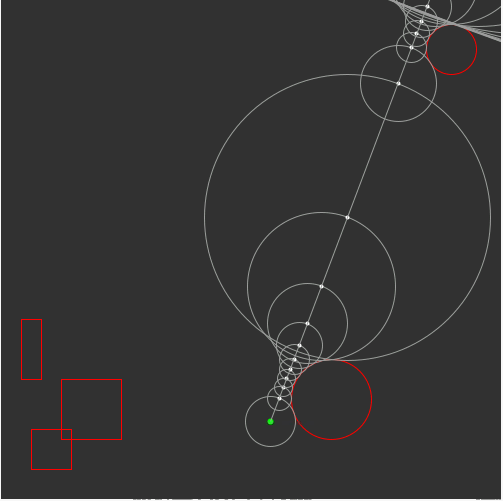
\includegraphics[width=8cm]{images/marching.png}
\begin{figure}[h]
    \centering
    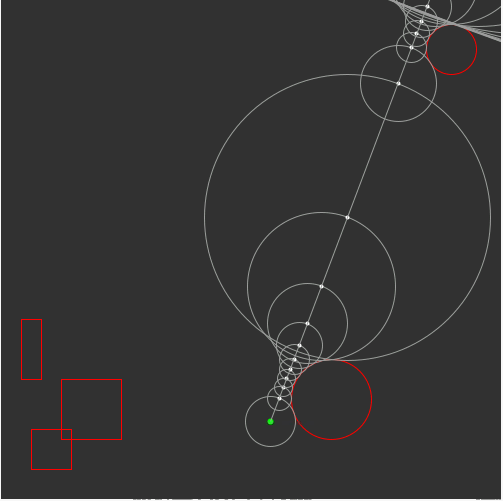
\includegraphics[width=8cm]{images/marching.png}
    \caption{Illustration 2D de la marche point par point d'un rayon (plus de details dans \ref{subsec:projection} \nameref{subsec:projection})}
    \label{fig:my_label}
\end{figure}

\clearpage
\documentclass[a4paper,11pt,twoside]{article} 
%\documentclass{article}


\author{Victor LASSERRE \& Valentin SERVIERES}
\pdfminorversion=7 % To use charte graphique (pdf 1.7)
\usepackage[utf8]{inputenc}
\usepackage[T1]{fontenc}
\usepackage{lscape}
\usepackage{boldline,multirow,tabularx,colortbl,makecell,fancybox,amsfonts,amssymb,amsmath,mathrsfs,array, svg}
\usepackage{pgf,tikz,xcolor,graphicx}
\usetikzlibrary{calc,positioning,shapes.geometric,shapes.symbols,shapes.misc, fit, shapes, arrows, arrows.meta,fadings,through}
\usepackage[top=2cm, bottom=2cm, left=2cm, right=2cm]{geometry}
\usepackage{hyperref,titlesec,eurosym,eso-pic,float}
\usepackage[french]{babel}
%\usepackage{bibleref} ajouté par moi mais flemme
% minted et les encars de code en gros
%\usepackage[newfloat]{minted}
\usepackage{caption}
\usepackage{tcolorbox}
%\newenvironment{code}{\captionsetup{type=listing}}{}
%\SetupFloatingEnvironment{listing}{name=Code Source}

% table des annexes
\usepackage{minitoc}
\usepackage{pdfpages}

% bibliographie
%\usepackage{biblatex}
%\usepackage{csquotes}
%\addbibresource{bibliography.bib}

%\input{advanced.params/listings.conf}
\input{charteINSA/advanced.params/tikz.conf}
\input{charteINSA/advanced.params/misc.commands}
\input{charteINSA/cover/covermain.tex}



%\usepackage[french]{babel}

% resolve no citation problem
\nocite{*}
%\usepackage[...,backend=bibtex]{biblatex}

% Set page size and margins
% Replace `letterpaper' with `a4paper' for UK/EU standard size
%%%%%\usepackage[letterpaper,top=2cm,bottom=2cm,left=3cm,right=3cm,marginparwidth=1.75cm]{geometry}

% Useful packages
\usepackage{listings}

\input{preferences/listings-glsl.prf}
% optionally set GLSL as default language
\lstset{language=GLSL}
\lstset{
  breaklines=true,
  breakatwhitespace=true,
  numbers=left,
  basicstyle={\small\ttfamily},
  numberstyle=\tiny\color{gray},
  tabsize=3,% end normal settings
  breaklines=true,                              % break long lines
  commentstyle=\itshape\color{green},           % comments are green
  keywordstyle=[1]\color{blue},                 % instructions are blue
  keywordstyle=[2]\color{orange},               % sections/other directives are orange
  keywordstyle=[3]\color{red},                   % registers are red
  stringstyle=\color{mauve},                    % strings are from the telekom
  identifierstyle=\color{teal},                 % user declared addresses are teal
  frame=l,                                      % black line on the left side of code
  language=GLSL,                   % all code is RISC-V
  tabsize=4,                                    % indent tabs with 4 spaces
  showstringspaces=false                        % do not replace spaces with weird underlines
}

\usepackage[square,numbers]{natbib}
\bibliographystyle{abbrvnat}
%Includes "References" in the table of contents
\usepackage[nottoc]{tocbibind}

\usepackage{setspace}
\usepackage{titletoc}
%\usepackage[T1]{fontenc}
%\usepackage{amsfonts}
%\usepackage{graphicx}
\usepackage{mathtools}
\graphicspath{ {images/} }

%\usepackage{fancyhdr}
\pagestyle{fancy}
\renewcommand\headrulewidth{1pt}
\fancyhead[L]{\textsf{Moteur graphique}}
\fancyhead[R]{\textsf{}}
%\usepackage[colorlinks=true, allcolors=blue]{hyperref}


\begin{document}
\dosecttoc{} % generate TOC
%\maketitle
\clearpage

% Remerciements
\thispagestyle{empty} % removes page number
\subsection*{Remerciements}
Nous tenons à remercier notre tuteur de projet M. Sanchez, notamment pour son aide précieuse et ses conseils. \\
Nous remercions également Inigo Quilez pour la riche documentation sur le ray marching qu'il fournit librement sur son site web.
\clearpage

% TABLE DES MATIÈRES
\thispagestyle{empty} % removes page number
\setcounter{secnumdepth}{3}
\tableofcontents
\clearpage

\setcounter{page}{1}


\sectionnn{Introduction}

    Engin Pas Tangible est un moteur graphique reposant sur le principe de Ray Marching : un système de 3D similaire au Ray Tracing, mais beaucoup plus rarement utilisé. Ce système a certains avantages par rapport au Ray Tracing, comme par exemple de permettre une implémetation peu coûteuse de fractales, ou autres figures se reproduisant à l'identique. \\
    Le Ray Marching repose sur la projection de rayons depuis une camera vers la scene. Pour projeter un rayon, on le fait avancer pas à pas (\emph{Marching}). La distance des pas doit être la plus grande possible, mais sans que le rayon ne traverse d'objet de la scene 3D.
\\
\\
%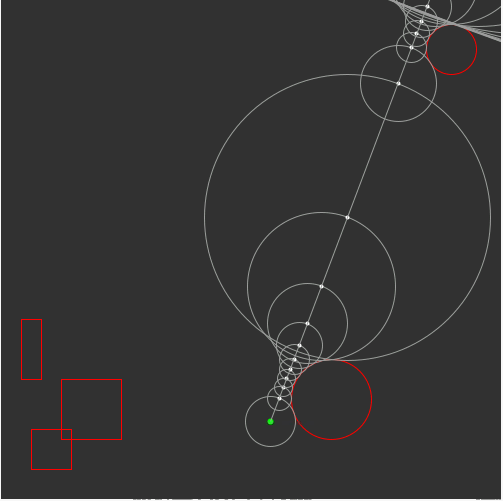
\includegraphics[width=8cm]{images/marching.png}
\begin{figure}[h]
    \centering
    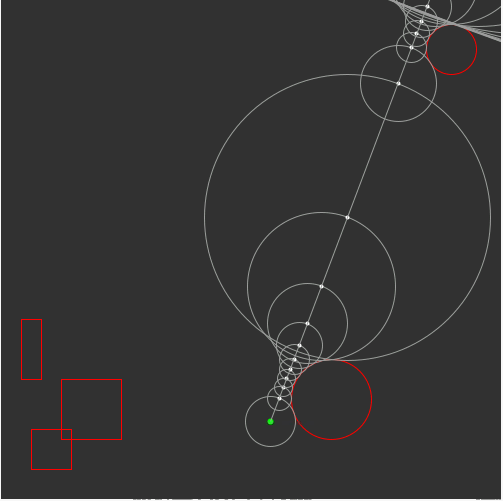
\includegraphics[width=8cm]{images/marching.png}
    \caption{Illustration 2D de la marche point par point d'un rayon (plus de details dans \ref{subsec:projection} \nameref{subsec:projection})}
    \label{fig:my_label}
\end{figure}

\clearpage
\documentclass[a4paper,11pt,twoside]{article} 
%\documentclass{article}

\input{charteINSA/maincharte.tex}

%\usepackage[french]{babel}

% resolve no citation problem
\nocite{*}
%\usepackage[...,backend=bibtex]{biblatex}

% Set page size and margins
% Replace `letterpaper' with `a4paper' for UK/EU standard size
%%%%%\usepackage[letterpaper,top=2cm,bottom=2cm,left=3cm,right=3cm,marginparwidth=1.75cm]{geometry}

% Useful packages
\usepackage{listings}

\input{preferences/listings-glsl.prf}
% optionally set GLSL as default language
\lstset{language=GLSL}
\input{preferences/glsl.tex}

\usepackage[square,numbers]{natbib}
\bibliographystyle{abbrvnat}
%Includes "References" in the table of contents
\usepackage[nottoc]{tocbibind}

\usepackage{setspace}
\usepackage{titletoc}
%\usepackage[T1]{fontenc}
%\usepackage{amsfonts}
%\usepackage{graphicx}
\usepackage{mathtools}
\graphicspath{ {images/} }

%\input{hautdepage.tex}
%\usepackage[colorlinks=true, allcolors=blue]{hyperref}


\begin{document}
\dosecttoc{} % generate TOC
%\maketitle
\clearpage

% Remerciements
\thispagestyle{empty} % removes page number
\subsection*{Remerciements}
Nous tenons à remercier notre tuteur de projet M. Sanchez, notamment pour son aide précieuse et ses conseils. \\
Nous remercions également Inigo Quilez pour la riche documentation sur le ray marching qu'il fournit librement sur son site web.
\clearpage

% TABLE DES MATIÈRES
\thispagestyle{empty} % removes page number
\setcounter{secnumdepth}{3}
\tableofcontents
\clearpage

\setcounter{page}{1}


\input{Parties/Introduction}
\clearpage
\input{Parties/Fonctionnement/main}
\clearpage
\input{Parties/Fonctionnalites/main}
\clearpage
\input{Parties/Historique/main}
\clearpage
\input{Parties/Conclusion}

\clearpage


%Imports the bibliography file "sample.bib"
\bibliography{sample}
\clearpage

% TABLE DES ANNEXES
\clearpage
\appendix
%\thispagestyle{empty} % removes page number
\sectionnn{Table des Annexes}
\addtocontents{toc}{\protect\setcounter{tocdepth}{0}}
\renewcommand{\stctitle}{}                          % Titre (issue with previous subsection showing up)
\renewcommand\thesubsection{A\arabic{subsection}}   % Numérotation
\renewcommand{\stcSSfont}{}                         % Police normale, pas en gras
\mtcsetrules{secttoc}{off}                          % Désactivation des lignes en haut et en bas de la table

% Affichage de la table des annexes
\secttoc
% ANNEXES
\clearpage
\pagenumbering{Roman}


\input{Parties/Annexes}

\mtcsetrules{secttoc}{off}

\end{document}


                        

\clearpage
\documentclass[a4paper,11pt,twoside]{article} 
%\documentclass{article}

\input{charteINSA/maincharte.tex}

%\usepackage[french]{babel}

% resolve no citation problem
\nocite{*}
%\usepackage[...,backend=bibtex]{biblatex}

% Set page size and margins
% Replace `letterpaper' with `a4paper' for UK/EU standard size
%%%%%\usepackage[letterpaper,top=2cm,bottom=2cm,left=3cm,right=3cm,marginparwidth=1.75cm]{geometry}

% Useful packages
\usepackage{listings}

\input{preferences/listings-glsl.prf}
% optionally set GLSL as default language
\lstset{language=GLSL}
\input{preferences/glsl.tex}

\usepackage[square,numbers]{natbib}
\bibliographystyle{abbrvnat}
%Includes "References" in the table of contents
\usepackage[nottoc]{tocbibind}

\usepackage{setspace}
\usepackage{titletoc}
%\usepackage[T1]{fontenc}
%\usepackage{amsfonts}
%\usepackage{graphicx}
\usepackage{mathtools}
\graphicspath{ {images/} }

%\input{hautdepage.tex}
%\usepackage[colorlinks=true, allcolors=blue]{hyperref}


\begin{document}
\dosecttoc{} % generate TOC
%\maketitle
\clearpage

% Remerciements
\thispagestyle{empty} % removes page number
\subsection*{Remerciements}
Nous tenons à remercier notre tuteur de projet M. Sanchez, notamment pour son aide précieuse et ses conseils. \\
Nous remercions également Inigo Quilez pour la riche documentation sur le ray marching qu'il fournit librement sur son site web.
\clearpage

% TABLE DES MATIÈRES
\thispagestyle{empty} % removes page number
\setcounter{secnumdepth}{3}
\tableofcontents
\clearpage

\setcounter{page}{1}


\input{Parties/Introduction}
\clearpage
\input{Parties/Fonctionnement/main}
\clearpage
\input{Parties/Fonctionnalites/main}
\clearpage
\input{Parties/Historique/main}
\clearpage
\input{Parties/Conclusion}

\clearpage


%Imports the bibliography file "sample.bib"
\bibliography{sample}
\clearpage

% TABLE DES ANNEXES
\clearpage
\appendix
%\thispagestyle{empty} % removes page number
\sectionnn{Table des Annexes}
\addtocontents{toc}{\protect\setcounter{tocdepth}{0}}
\renewcommand{\stctitle}{}                          % Titre (issue with previous subsection showing up)
\renewcommand\thesubsection{A\arabic{subsection}}   % Numérotation
\renewcommand{\stcSSfont}{}                         % Police normale, pas en gras
\mtcsetrules{secttoc}{off}                          % Désactivation des lignes en haut et en bas de la table

% Affichage de la table des annexes
\secttoc
% ANNEXES
\clearpage
\pagenumbering{Roman}


\input{Parties/Annexes}

\mtcsetrules{secttoc}{off}

\end{document}


                        

\clearpage
\documentclass[a4paper,11pt,twoside]{article} 
%\documentclass{article}

\input{charteINSA/maincharte.tex}

%\usepackage[french]{babel}

% resolve no citation problem
\nocite{*}
%\usepackage[...,backend=bibtex]{biblatex}

% Set page size and margins
% Replace `letterpaper' with `a4paper' for UK/EU standard size
%%%%%\usepackage[letterpaper,top=2cm,bottom=2cm,left=3cm,right=3cm,marginparwidth=1.75cm]{geometry}

% Useful packages
\usepackage{listings}

\input{preferences/listings-glsl.prf}
% optionally set GLSL as default language
\lstset{language=GLSL}
\input{preferences/glsl.tex}

\usepackage[square,numbers]{natbib}
\bibliographystyle{abbrvnat}
%Includes "References" in the table of contents
\usepackage[nottoc]{tocbibind}

\usepackage{setspace}
\usepackage{titletoc}
%\usepackage[T1]{fontenc}
%\usepackage{amsfonts}
%\usepackage{graphicx}
\usepackage{mathtools}
\graphicspath{ {images/} }

%\input{hautdepage.tex}
%\usepackage[colorlinks=true, allcolors=blue]{hyperref}


\begin{document}
\dosecttoc{} % generate TOC
%\maketitle
\clearpage

% Remerciements
\thispagestyle{empty} % removes page number
\subsection*{Remerciements}
Nous tenons à remercier notre tuteur de projet M. Sanchez, notamment pour son aide précieuse et ses conseils. \\
Nous remercions également Inigo Quilez pour la riche documentation sur le ray marching qu'il fournit librement sur son site web.
\clearpage

% TABLE DES MATIÈRES
\thispagestyle{empty} % removes page number
\setcounter{secnumdepth}{3}
\tableofcontents
\clearpage

\setcounter{page}{1}


\input{Parties/Introduction}
\clearpage
\input{Parties/Fonctionnement/main}
\clearpage
\input{Parties/Fonctionnalites/main}
\clearpage
\input{Parties/Historique/main}
\clearpage
\input{Parties/Conclusion}

\clearpage


%Imports the bibliography file "sample.bib"
\bibliography{sample}
\clearpage

% TABLE DES ANNEXES
\clearpage
\appendix
%\thispagestyle{empty} % removes page number
\sectionnn{Table des Annexes}
\addtocontents{toc}{\protect\setcounter{tocdepth}{0}}
\renewcommand{\stctitle}{}                          % Titre (issue with previous subsection showing up)
\renewcommand\thesubsection{A\arabic{subsection}}   % Numérotation
\renewcommand{\stcSSfont}{}                         % Police normale, pas en gras
\mtcsetrules{secttoc}{off}                          % Désactivation des lignes en haut et en bas de la table

% Affichage de la table des annexes
\secttoc
% ANNEXES
\clearpage
\pagenumbering{Roman}


\input{Parties/Annexes}

\mtcsetrules{secttoc}{off}

\end{document}


                        

\clearpage
\sectionnn{Conclusion}

Ce projet a été captivant et très motivant. Le fait de pouvoir observer rapidement les résultats de notre code était très agréable.\\
Nous avons rempli et même dépassé les objectifs que nous nous étions fixés.\\
Il était également intéressant de retrouver des notions vues en maths à l'INSA dans une application concrète.\\ \par

L'expérience fut très enrichissante car nous avons dû nous organiser pour pouvoir travailler en binôme sur le même code avec l'utilisation d'un gestionnaire de version (git) auquel nous nous sommes formés.\\
Nous avons pu explorer le principe du Ray Marching, découvrir un nouveau langage, le GLSL, ainsi que les bases de développement logiciel.\\ \par

Ce rapport était également l'occasion d'apprendre à maîtriser le LaTeX, mais c'était surtout l'occasion d'expliquer de façon claire et concise un concept technique.\\ \par

Finalement, ce projet de moteur graphique nous a beaucoup apporté et nous pensons continuer à le développer dans le futur.

\clearpage


%Imports the bibliography file "sample.bib"
\bibliography{sample}
\clearpage

% TABLE DES ANNEXES
\clearpage
\appendix
%\thispagestyle{empty} % removes page number
\sectionnn{Table des Annexes}
\addtocontents{toc}{\protect\setcounter{tocdepth}{0}}
\renewcommand{\stctitle}{}                          % Titre (issue with previous subsection showing up)
\renewcommand\thesubsection{A\arabic{subsection}}   % Numérotation
\renewcommand{\stcSSfont}{}                         % Police normale, pas en gras
\mtcsetrules{secttoc}{off}                          % Désactivation des lignes en haut et en bas de la table

% Affichage de la table des annexes
\secttoc
% ANNEXES
\clearpage
\pagenumbering{Roman}


\subsection{Scène simple}
%\addcontentsline{toc}{section}{Scène simple}
Code à mettre dans un fichier, nommé \emph{example.fs} par exemple
\begin{lstlisting}[language=GLSL]
#version 330 core
in vec2 FragCoord;
in float Time;
in vec2 MousePos;
in vec3 CamPos;
in vec3 CamDir;

out vec4 FragColor;
//uniform sampler2D generalTexture;

float SDF_Box_Frame( vec3 p, vec3 b, float e )
{
       p = abs(p  )-b;
  vec3 q = abs(p+e)-e;
  return min(min(
      length(max(vec3(p.x,q.y,q.z),0.0))+min(max(p.x,max(q.y,q.z)),0.0),
      length(max(vec3(q.x,p.y,q.z),0.0))+min(max(q.x,max(p.y,q.z)),0.0)),
      length(max(vec3(q.x,q.y,p.z),0.0))+min(max(q.x,max(q.y,p.z)),0.0));
}

float SDF_Circle(vec3 p,float r){
    return length(p)-r;
}

float SDF_Global(vec3 p){
    return min(
        SDF_Box_Frame(p,vec3(.5,.5,.5),0.1),
        SDF_Circle(mod(p+vec3(.5),vec3(1.,1.,1.))-vec3(.5),.15));
}

vec4 Get_Impact(vec3 origin,vec3 dir){//must have length(dir)==1 
    vec3 pos=origin;
    float dist;
    for(int i=0;i<30;i++){
        dist=SDF_Global(pos);
        pos+=dist*dir;
        if(dist<=.01) return vec4(pos,1.);
        if(dist>=20.0) return vec4(pos,-1.);
    }
    return vec4(pos,-1.);
}

vec3 grad(vec3 p){
    vec2 epsilon = vec2(.01,0.);
    return normalize(vec3(SDF_Global(p+epsilon.xyy)-SDF_Global(p-epsilon.xyy),
    SDF_Global(p+epsilon.yxy)-SDF_Global(p-epsilon.yxy),
    SDF_Global(p+epsilon.yyx)-SDF_Global(p-epsilon.yyx)));
}

vec3 Get_Color(vec3 origin,vec3 dir){
    vec4 impact = Get_Impact(origin,dir);
    if(impact.w<0.) return vec3(.5,.7,1.);
    vec3 normale=grad(impact.xyz);
    return normale;
}

void main()
{
    vec3 lookingAt = vec3(0.,0.,0.);
    vec3 posCam    = vec3(3.*sin(Time*.5),0.,3.*cos(Time*.5));
    
    vec3 ez = normalize(lookingAt - posCam); //base orthonormee
    vec3 ex = normalize(cross(ez,vec3(0.,1.,0.)));
    vec3 ey = cross(ex,ez);
    
    vec3 dir = normalize(FragCoord.x * ex + FragCoord.y*ey + 1.*ez);
    
  FragColor=vec4(Get_Color(posCam,dir),1.);
}
\end{lstlisting}

\mtcsetrules{secttoc}{off}

\end{document}


                        

\clearpage
\documentclass[a4paper,11pt,twoside]{article} 
%\documentclass{article}


\author{Victor LASSERRE \& Valentin SERVIERES}
\pdfminorversion=7 % To use charte graphique (pdf 1.7)
\usepackage[utf8]{inputenc}
\usepackage[T1]{fontenc}
\usepackage{lscape}
\usepackage{boldline,multirow,tabularx,colortbl,makecell,fancybox,amsfonts,amssymb,amsmath,mathrsfs,array, svg}
\usepackage{pgf,tikz,xcolor,graphicx}
\usetikzlibrary{calc,positioning,shapes.geometric,shapes.symbols,shapes.misc, fit, shapes, arrows, arrows.meta,fadings,through}
\usepackage[top=2cm, bottom=2cm, left=2cm, right=2cm]{geometry}
\usepackage{hyperref,titlesec,eurosym,eso-pic,float}
\usepackage[french]{babel}
%\usepackage{bibleref} ajouté par moi mais flemme
% minted et les encars de code en gros
%\usepackage[newfloat]{minted}
\usepackage{caption}
\usepackage{tcolorbox}
%\newenvironment{code}{\captionsetup{type=listing}}{}
%\SetupFloatingEnvironment{listing}{name=Code Source}

% table des annexes
\usepackage{minitoc}
\usepackage{pdfpages}

% bibliographie
%\usepackage{biblatex}
%\usepackage{csquotes}
%\addbibresource{bibliography.bib}

%\input{advanced.params/listings.conf}
\input{charteINSA/advanced.params/tikz.conf}
\input{charteINSA/advanced.params/misc.commands}
\input{charteINSA/cover/covermain.tex}



%\usepackage[french]{babel}

% resolve no citation problem
\nocite{*}
%\usepackage[...,backend=bibtex]{biblatex}

% Set page size and margins
% Replace `letterpaper' with `a4paper' for UK/EU standard size
%%%%%\usepackage[letterpaper,top=2cm,bottom=2cm,left=3cm,right=3cm,marginparwidth=1.75cm]{geometry}

% Useful packages
\usepackage{listings}

\input{preferences/listings-glsl.prf}
% optionally set GLSL as default language
\lstset{language=GLSL}
\lstset{
  breaklines=true,
  breakatwhitespace=true,
  numbers=left,
  basicstyle={\small\ttfamily},
  numberstyle=\tiny\color{gray},
  tabsize=3,% end normal settings
  breaklines=true,                              % break long lines
  commentstyle=\itshape\color{green},           % comments are green
  keywordstyle=[1]\color{blue},                 % instructions are blue
  keywordstyle=[2]\color{orange},               % sections/other directives are orange
  keywordstyle=[3]\color{red},                   % registers are red
  stringstyle=\color{mauve},                    % strings are from the telekom
  identifierstyle=\color{teal},                 % user declared addresses are teal
  frame=l,                                      % black line on the left side of code
  language=GLSL,                   % all code is RISC-V
  tabsize=4,                                    % indent tabs with 4 spaces
  showstringspaces=false                        % do not replace spaces with weird underlines
}

\usepackage[square,numbers]{natbib}
\bibliographystyle{abbrvnat}
%Includes "References" in the table of contents
\usepackage[nottoc]{tocbibind}

\usepackage{setspace}
\usepackage{titletoc}
%\usepackage[T1]{fontenc}
%\usepackage{amsfonts}
%\usepackage{graphicx}
\usepackage{mathtools}
\graphicspath{ {images/} }

%\usepackage{fancyhdr}
\pagestyle{fancy}
\renewcommand\headrulewidth{1pt}
\fancyhead[L]{\textsf{Moteur graphique}}
\fancyhead[R]{\textsf{}}
%\usepackage[colorlinks=true, allcolors=blue]{hyperref}


\begin{document}
\dosecttoc{} % generate TOC
%\maketitle
\clearpage

% Remerciements
\thispagestyle{empty} % removes page number
\subsection*{Remerciements}
Nous tenons à remercier notre tuteur de projet M. Sanchez, notamment pour son aide précieuse et ses conseils. \\
Nous remercions également Inigo Quilez pour la riche documentation sur le ray marching qu'il fournit librement sur son site web.
\clearpage

% TABLE DES MATIÈRES
\thispagestyle{empty} % removes page number
\setcounter{secnumdepth}{3}
\tableofcontents
\clearpage

\setcounter{page}{1}


\sectionnn{Introduction}

    Engin Pas Tangible est un moteur graphique reposant sur le principe de Ray Marching : un système de 3D similaire au Ray Tracing, mais beaucoup plus rarement utilisé. Ce système a certains avantages par rapport au Ray Tracing, comme par exemple de permettre une implémetation peu coûteuse de fractales, ou autres figures se reproduisant à l'identique. \\
    Le Ray Marching repose sur la projection de rayons depuis une camera vers la scene. Pour projeter un rayon, on le fait avancer pas à pas (\emph{Marching}). La distance des pas doit être la plus grande possible, mais sans que le rayon ne traverse d'objet de la scene 3D.
\\
\\
%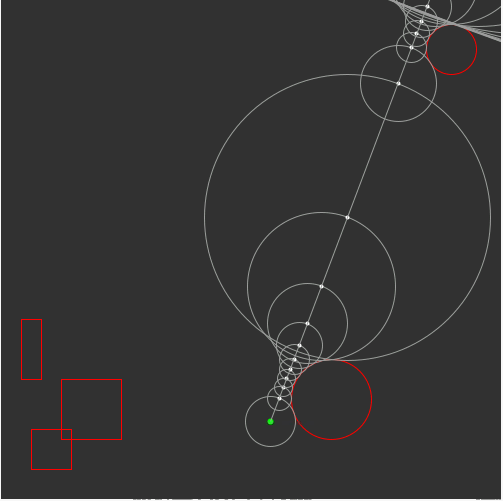
\includegraphics[width=8cm]{images/marching.png}
\begin{figure}[h]
    \centering
    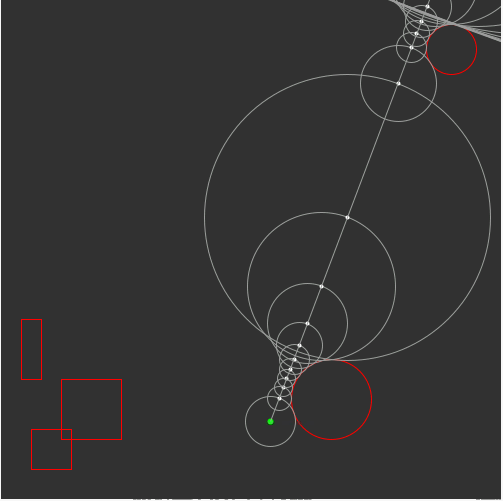
\includegraphics[width=8cm]{images/marching.png}
    \caption{Illustration 2D de la marche point par point d'un rayon (plus de details dans \ref{subsec:projection} \nameref{subsec:projection})}
    \label{fig:my_label}
\end{figure}

\clearpage
\documentclass[a4paper,11pt,twoside]{article} 
%\documentclass{article}

\input{charteINSA/maincharte.tex}

%\usepackage[french]{babel}

% resolve no citation problem
\nocite{*}
%\usepackage[...,backend=bibtex]{biblatex}

% Set page size and margins
% Replace `letterpaper' with `a4paper' for UK/EU standard size
%%%%%\usepackage[letterpaper,top=2cm,bottom=2cm,left=3cm,right=3cm,marginparwidth=1.75cm]{geometry}

% Useful packages
\usepackage{listings}

\input{preferences/listings-glsl.prf}
% optionally set GLSL as default language
\lstset{language=GLSL}
\input{preferences/glsl.tex}

\usepackage[square,numbers]{natbib}
\bibliographystyle{abbrvnat}
%Includes "References" in the table of contents
\usepackage[nottoc]{tocbibind}

\usepackage{setspace}
\usepackage{titletoc}
%\usepackage[T1]{fontenc}
%\usepackage{amsfonts}
%\usepackage{graphicx}
\usepackage{mathtools}
\graphicspath{ {images/} }

%\input{hautdepage.tex}
%\usepackage[colorlinks=true, allcolors=blue]{hyperref}


\begin{document}
\dosecttoc{} % generate TOC
%\maketitle
\clearpage

% Remerciements
\thispagestyle{empty} % removes page number
\subsection*{Remerciements}
Nous tenons à remercier notre tuteur de projet M. Sanchez, notamment pour son aide précieuse et ses conseils. \\
Nous remercions également Inigo Quilez pour la riche documentation sur le ray marching qu'il fournit librement sur son site web.
\clearpage

% TABLE DES MATIÈRES
\thispagestyle{empty} % removes page number
\setcounter{secnumdepth}{3}
\tableofcontents
\clearpage

\setcounter{page}{1}


\input{Parties/Introduction}
\clearpage
\input{Parties/Fonctionnement/main}
\clearpage
\input{Parties/Fonctionnalites/main}
\clearpage
\input{Parties/Historique/main}
\clearpage
\input{Parties/Conclusion}

\clearpage


%Imports the bibliography file "sample.bib"
\bibliography{sample}
\clearpage

% TABLE DES ANNEXES
\clearpage
\appendix
%\thispagestyle{empty} % removes page number
\sectionnn{Table des Annexes}
\addtocontents{toc}{\protect\setcounter{tocdepth}{0}}
\renewcommand{\stctitle}{}                          % Titre (issue with previous subsection showing up)
\renewcommand\thesubsection{A\arabic{subsection}}   % Numérotation
\renewcommand{\stcSSfont}{}                         % Police normale, pas en gras
\mtcsetrules{secttoc}{off}                          % Désactivation des lignes en haut et en bas de la table

% Affichage de la table des annexes
\secttoc
% ANNEXES
\clearpage
\pagenumbering{Roman}


\input{Parties/Annexes}

\mtcsetrules{secttoc}{off}

\end{document}


                        

\clearpage
\documentclass[a4paper,11pt,twoside]{article} 
%\documentclass{article}

\input{charteINSA/maincharte.tex}

%\usepackage[french]{babel}

% resolve no citation problem
\nocite{*}
%\usepackage[...,backend=bibtex]{biblatex}

% Set page size and margins
% Replace `letterpaper' with `a4paper' for UK/EU standard size
%%%%%\usepackage[letterpaper,top=2cm,bottom=2cm,left=3cm,right=3cm,marginparwidth=1.75cm]{geometry}

% Useful packages
\usepackage{listings}

\input{preferences/listings-glsl.prf}
% optionally set GLSL as default language
\lstset{language=GLSL}
\input{preferences/glsl.tex}

\usepackage[square,numbers]{natbib}
\bibliographystyle{abbrvnat}
%Includes "References" in the table of contents
\usepackage[nottoc]{tocbibind}

\usepackage{setspace}
\usepackage{titletoc}
%\usepackage[T1]{fontenc}
%\usepackage{amsfonts}
%\usepackage{graphicx}
\usepackage{mathtools}
\graphicspath{ {images/} }

%\input{hautdepage.tex}
%\usepackage[colorlinks=true, allcolors=blue]{hyperref}


\begin{document}
\dosecttoc{} % generate TOC
%\maketitle
\clearpage

% Remerciements
\thispagestyle{empty} % removes page number
\subsection*{Remerciements}
Nous tenons à remercier notre tuteur de projet M. Sanchez, notamment pour son aide précieuse et ses conseils. \\
Nous remercions également Inigo Quilez pour la riche documentation sur le ray marching qu'il fournit librement sur son site web.
\clearpage

% TABLE DES MATIÈRES
\thispagestyle{empty} % removes page number
\setcounter{secnumdepth}{3}
\tableofcontents
\clearpage

\setcounter{page}{1}


\input{Parties/Introduction}
\clearpage
\input{Parties/Fonctionnement/main}
\clearpage
\input{Parties/Fonctionnalites/main}
\clearpage
\input{Parties/Historique/main}
\clearpage
\input{Parties/Conclusion}

\clearpage


%Imports the bibliography file "sample.bib"
\bibliography{sample}
\clearpage

% TABLE DES ANNEXES
\clearpage
\appendix
%\thispagestyle{empty} % removes page number
\sectionnn{Table des Annexes}
\addtocontents{toc}{\protect\setcounter{tocdepth}{0}}
\renewcommand{\stctitle}{}                          % Titre (issue with previous subsection showing up)
\renewcommand\thesubsection{A\arabic{subsection}}   % Numérotation
\renewcommand{\stcSSfont}{}                         % Police normale, pas en gras
\mtcsetrules{secttoc}{off}                          % Désactivation des lignes en haut et en bas de la table

% Affichage de la table des annexes
\secttoc
% ANNEXES
\clearpage
\pagenumbering{Roman}


\input{Parties/Annexes}

\mtcsetrules{secttoc}{off}

\end{document}


                        

\clearpage
\documentclass[a4paper,11pt,twoside]{article} 
%\documentclass{article}

\input{charteINSA/maincharte.tex}

%\usepackage[french]{babel}

% resolve no citation problem
\nocite{*}
%\usepackage[...,backend=bibtex]{biblatex}

% Set page size and margins
% Replace `letterpaper' with `a4paper' for UK/EU standard size
%%%%%\usepackage[letterpaper,top=2cm,bottom=2cm,left=3cm,right=3cm,marginparwidth=1.75cm]{geometry}

% Useful packages
\usepackage{listings}

\input{preferences/listings-glsl.prf}
% optionally set GLSL as default language
\lstset{language=GLSL}
\input{preferences/glsl.tex}

\usepackage[square,numbers]{natbib}
\bibliographystyle{abbrvnat}
%Includes "References" in the table of contents
\usepackage[nottoc]{tocbibind}

\usepackage{setspace}
\usepackage{titletoc}
%\usepackage[T1]{fontenc}
%\usepackage{amsfonts}
%\usepackage{graphicx}
\usepackage{mathtools}
\graphicspath{ {images/} }

%\input{hautdepage.tex}
%\usepackage[colorlinks=true, allcolors=blue]{hyperref}


\begin{document}
\dosecttoc{} % generate TOC
%\maketitle
\clearpage

% Remerciements
\thispagestyle{empty} % removes page number
\subsection*{Remerciements}
Nous tenons à remercier notre tuteur de projet M. Sanchez, notamment pour son aide précieuse et ses conseils. \\
Nous remercions également Inigo Quilez pour la riche documentation sur le ray marching qu'il fournit librement sur son site web.
\clearpage

% TABLE DES MATIÈRES
\thispagestyle{empty} % removes page number
\setcounter{secnumdepth}{3}
\tableofcontents
\clearpage

\setcounter{page}{1}


\input{Parties/Introduction}
\clearpage
\input{Parties/Fonctionnement/main}
\clearpage
\input{Parties/Fonctionnalites/main}
\clearpage
\input{Parties/Historique/main}
\clearpage
\input{Parties/Conclusion}

\clearpage


%Imports the bibliography file "sample.bib"
\bibliography{sample}
\clearpage

% TABLE DES ANNEXES
\clearpage
\appendix
%\thispagestyle{empty} % removes page number
\sectionnn{Table des Annexes}
\addtocontents{toc}{\protect\setcounter{tocdepth}{0}}
\renewcommand{\stctitle}{}                          % Titre (issue with previous subsection showing up)
\renewcommand\thesubsection{A\arabic{subsection}}   % Numérotation
\renewcommand{\stcSSfont}{}                         % Police normale, pas en gras
\mtcsetrules{secttoc}{off}                          % Désactivation des lignes en haut et en bas de la table

% Affichage de la table des annexes
\secttoc
% ANNEXES
\clearpage
\pagenumbering{Roman}


\input{Parties/Annexes}

\mtcsetrules{secttoc}{off}

\end{document}


                        

\clearpage
\sectionnn{Conclusion}

Ce projet a été captivant et très motivant. Le fait de pouvoir observer rapidement les résultats de notre code était très agréable.\\
Nous avons rempli et même dépassé les objectifs que nous nous étions fixés.\\
Il était également intéressant de retrouver des notions vues en maths à l'INSA dans une application concrète.\\ \par

L'expérience fut très enrichissante car nous avons dû nous organiser pour pouvoir travailler en binôme sur le même code avec l'utilisation d'un gestionnaire de version (git) auquel nous nous sommes formés.\\
Nous avons pu explorer le principe du Ray Marching, découvrir un nouveau langage, le GLSL, ainsi que les bases de développement logiciel.\\ \par

Ce rapport était également l'occasion d'apprendre à maîtriser le LaTeX, mais c'était surtout l'occasion d'expliquer de façon claire et concise un concept technique.\\ \par

Finalement, ce projet de moteur graphique nous a beaucoup apporté et nous pensons continuer à le développer dans le futur.

\clearpage


%Imports the bibliography file "sample.bib"
\bibliography{sample}
\clearpage

% TABLE DES ANNEXES
\clearpage
\appendix
%\thispagestyle{empty} % removes page number
\sectionnn{Table des Annexes}
\addtocontents{toc}{\protect\setcounter{tocdepth}{0}}
\renewcommand{\stctitle}{}                          % Titre (issue with previous subsection showing up)
\renewcommand\thesubsection{A\arabic{subsection}}   % Numérotation
\renewcommand{\stcSSfont}{}                         % Police normale, pas en gras
\mtcsetrules{secttoc}{off}                          % Désactivation des lignes en haut et en bas de la table

% Affichage de la table des annexes
\secttoc
% ANNEXES
\clearpage
\pagenumbering{Roman}


\subsection{Scène simple}
%\addcontentsline{toc}{section}{Scène simple}
Code à mettre dans un fichier, nommé \emph{example.fs} par exemple
\begin{lstlisting}[language=GLSL]
#version 330 core
in vec2 FragCoord;
in float Time;
in vec2 MousePos;
in vec3 CamPos;
in vec3 CamDir;

out vec4 FragColor;
//uniform sampler2D generalTexture;

float SDF_Box_Frame( vec3 p, vec3 b, float e )
{
       p = abs(p  )-b;
  vec3 q = abs(p+e)-e;
  return min(min(
      length(max(vec3(p.x,q.y,q.z),0.0))+min(max(p.x,max(q.y,q.z)),0.0),
      length(max(vec3(q.x,p.y,q.z),0.0))+min(max(q.x,max(p.y,q.z)),0.0)),
      length(max(vec3(q.x,q.y,p.z),0.0))+min(max(q.x,max(q.y,p.z)),0.0));
}

float SDF_Circle(vec3 p,float r){
    return length(p)-r;
}

float SDF_Global(vec3 p){
    return min(
        SDF_Box_Frame(p,vec3(.5,.5,.5),0.1),
        SDF_Circle(mod(p+vec3(.5),vec3(1.,1.,1.))-vec3(.5),.15));
}

vec4 Get_Impact(vec3 origin,vec3 dir){//must have length(dir)==1 
    vec3 pos=origin;
    float dist;
    for(int i=0;i<30;i++){
        dist=SDF_Global(pos);
        pos+=dist*dir;
        if(dist<=.01) return vec4(pos,1.);
        if(dist>=20.0) return vec4(pos,-1.);
    }
    return vec4(pos,-1.);
}

vec3 grad(vec3 p){
    vec2 epsilon = vec2(.01,0.);
    return normalize(vec3(SDF_Global(p+epsilon.xyy)-SDF_Global(p-epsilon.xyy),
    SDF_Global(p+epsilon.yxy)-SDF_Global(p-epsilon.yxy),
    SDF_Global(p+epsilon.yyx)-SDF_Global(p-epsilon.yyx)));
}

vec3 Get_Color(vec3 origin,vec3 dir){
    vec4 impact = Get_Impact(origin,dir);
    if(impact.w<0.) return vec3(.5,.7,1.);
    vec3 normale=grad(impact.xyz);
    return normale;
}

void main()
{
    vec3 lookingAt = vec3(0.,0.,0.);
    vec3 posCam    = vec3(3.*sin(Time*.5),0.,3.*cos(Time*.5));
    
    vec3 ez = normalize(lookingAt - posCam); //base orthonormee
    vec3 ex = normalize(cross(ez,vec3(0.,1.,0.)));
    vec3 ey = cross(ex,ez);
    
    vec3 dir = normalize(FragCoord.x * ex + FragCoord.y*ey + 1.*ez);
    
  FragColor=vec4(Get_Color(posCam,dir),1.);
}
\end{lstlisting}

\mtcsetrules{secttoc}{off}

\end{document}


                        

\clearpage
\documentclass[a4paper,11pt,twoside]{article} 
%\documentclass{article}


\author{Victor LASSERRE \& Valentin SERVIERES}
\pdfminorversion=7 % To use charte graphique (pdf 1.7)
\usepackage[utf8]{inputenc}
\usepackage[T1]{fontenc}
\usepackage{lscape}
\usepackage{boldline,multirow,tabularx,colortbl,makecell,fancybox,amsfonts,amssymb,amsmath,mathrsfs,array, svg}
\usepackage{pgf,tikz,xcolor,graphicx}
\usetikzlibrary{calc,positioning,shapes.geometric,shapes.symbols,shapes.misc, fit, shapes, arrows, arrows.meta,fadings,through}
\usepackage[top=2cm, bottom=2cm, left=2cm, right=2cm]{geometry}
\usepackage{hyperref,titlesec,eurosym,eso-pic,float}
\usepackage[french]{babel}
%\usepackage{bibleref} ajouté par moi mais flemme
% minted et les encars de code en gros
%\usepackage[newfloat]{minted}
\usepackage{caption}
\usepackage{tcolorbox}
%\newenvironment{code}{\captionsetup{type=listing}}{}
%\SetupFloatingEnvironment{listing}{name=Code Source}

% table des annexes
\usepackage{minitoc}
\usepackage{pdfpages}

% bibliographie
%\usepackage{biblatex}
%\usepackage{csquotes}
%\addbibresource{bibliography.bib}

%\input{advanced.params/listings.conf}
\input{charteINSA/advanced.params/tikz.conf}
\input{charteINSA/advanced.params/misc.commands}
\input{charteINSA/cover/covermain.tex}



%\usepackage[french]{babel}

% resolve no citation problem
\nocite{*}
%\usepackage[...,backend=bibtex]{biblatex}

% Set page size and margins
% Replace `letterpaper' with `a4paper' for UK/EU standard size
%%%%%\usepackage[letterpaper,top=2cm,bottom=2cm,left=3cm,right=3cm,marginparwidth=1.75cm]{geometry}

% Useful packages
\usepackage{listings}

\input{preferences/listings-glsl.prf}
% optionally set GLSL as default language
\lstset{language=GLSL}
\lstset{
  breaklines=true,
  breakatwhitespace=true,
  numbers=left,
  basicstyle={\small\ttfamily},
  numberstyle=\tiny\color{gray},
  tabsize=3,% end normal settings
  breaklines=true,                              % break long lines
  commentstyle=\itshape\color{green},           % comments are green
  keywordstyle=[1]\color{blue},                 % instructions are blue
  keywordstyle=[2]\color{orange},               % sections/other directives are orange
  keywordstyle=[3]\color{red},                   % registers are red
  stringstyle=\color{mauve},                    % strings are from the telekom
  identifierstyle=\color{teal},                 % user declared addresses are teal
  frame=l,                                      % black line on the left side of code
  language=GLSL,                   % all code is RISC-V
  tabsize=4,                                    % indent tabs with 4 spaces
  showstringspaces=false                        % do not replace spaces with weird underlines
}

\usepackage[square,numbers]{natbib}
\bibliographystyle{abbrvnat}
%Includes "References" in the table of contents
\usepackage[nottoc]{tocbibind}

\usepackage{setspace}
\usepackage{titletoc}
%\usepackage[T1]{fontenc}
%\usepackage{amsfonts}
%\usepackage{graphicx}
\usepackage{mathtools}
\graphicspath{ {images/} }

%\usepackage{fancyhdr}
\pagestyle{fancy}
\renewcommand\headrulewidth{1pt}
\fancyhead[L]{\textsf{Moteur graphique}}
\fancyhead[R]{\textsf{}}
%\usepackage[colorlinks=true, allcolors=blue]{hyperref}


\begin{document}
\dosecttoc{} % generate TOC
%\maketitle
\clearpage

% Remerciements
\thispagestyle{empty} % removes page number
\subsection*{Remerciements}
Nous tenons à remercier notre tuteur de projet M. Sanchez, notamment pour son aide précieuse et ses conseils. \\
Nous remercions également Inigo Quilez pour la riche documentation sur le ray marching qu'il fournit librement sur son site web.
\clearpage

% TABLE DES MATIÈRES
\thispagestyle{empty} % removes page number
\setcounter{secnumdepth}{3}
\tableofcontents
\clearpage

\setcounter{page}{1}


\sectionnn{Introduction}

    Engin Pas Tangible est un moteur graphique reposant sur le principe de Ray Marching : un système de 3D similaire au Ray Tracing, mais beaucoup plus rarement utilisé. Ce système a certains avantages par rapport au Ray Tracing, comme par exemple de permettre une implémetation peu coûteuse de fractales, ou autres figures se reproduisant à l'identique. \\
    Le Ray Marching repose sur la projection de rayons depuis une camera vers la scene. Pour projeter un rayon, on le fait avancer pas à pas (\emph{Marching}). La distance des pas doit être la plus grande possible, mais sans que le rayon ne traverse d'objet de la scene 3D.
\\
\\
%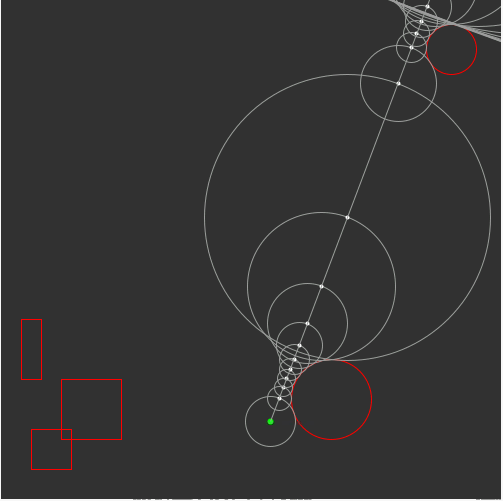
\includegraphics[width=8cm]{images/marching.png}
\begin{figure}[h]
    \centering
    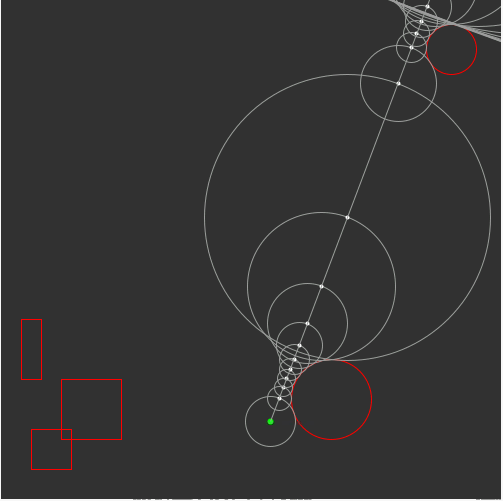
\includegraphics[width=8cm]{images/marching.png}
    \caption{Illustration 2D de la marche point par point d'un rayon (plus de details dans \ref{subsec:projection} \nameref{subsec:projection})}
    \label{fig:my_label}
\end{figure}

\clearpage
\documentclass[a4paper,11pt,twoside]{article} 
%\documentclass{article}

\input{charteINSA/maincharte.tex}

%\usepackage[french]{babel}

% resolve no citation problem
\nocite{*}
%\usepackage[...,backend=bibtex]{biblatex}

% Set page size and margins
% Replace `letterpaper' with `a4paper' for UK/EU standard size
%%%%%\usepackage[letterpaper,top=2cm,bottom=2cm,left=3cm,right=3cm,marginparwidth=1.75cm]{geometry}

% Useful packages
\usepackage{listings}

\input{preferences/listings-glsl.prf}
% optionally set GLSL as default language
\lstset{language=GLSL}
\input{preferences/glsl.tex}

\usepackage[square,numbers]{natbib}
\bibliographystyle{abbrvnat}
%Includes "References" in the table of contents
\usepackage[nottoc]{tocbibind}

\usepackage{setspace}
\usepackage{titletoc}
%\usepackage[T1]{fontenc}
%\usepackage{amsfonts}
%\usepackage{graphicx}
\usepackage{mathtools}
\graphicspath{ {images/} }

%\input{hautdepage.tex}
%\usepackage[colorlinks=true, allcolors=blue]{hyperref}


\begin{document}
\dosecttoc{} % generate TOC
%\maketitle
\clearpage

% Remerciements
\thispagestyle{empty} % removes page number
\subsection*{Remerciements}
Nous tenons à remercier notre tuteur de projet M. Sanchez, notamment pour son aide précieuse et ses conseils. \\
Nous remercions également Inigo Quilez pour la riche documentation sur le ray marching qu'il fournit librement sur son site web.
\clearpage

% TABLE DES MATIÈRES
\thispagestyle{empty} % removes page number
\setcounter{secnumdepth}{3}
\tableofcontents
\clearpage

\setcounter{page}{1}


\input{Parties/Introduction}
\clearpage
\input{Parties/Fonctionnement/main}
\clearpage
\input{Parties/Fonctionnalites/main}
\clearpage
\input{Parties/Historique/main}
\clearpage
\input{Parties/Conclusion}

\clearpage


%Imports the bibliography file "sample.bib"
\bibliography{sample}
\clearpage

% TABLE DES ANNEXES
\clearpage
\appendix
%\thispagestyle{empty} % removes page number
\sectionnn{Table des Annexes}
\addtocontents{toc}{\protect\setcounter{tocdepth}{0}}
\renewcommand{\stctitle}{}                          % Titre (issue with previous subsection showing up)
\renewcommand\thesubsection{A\arabic{subsection}}   % Numérotation
\renewcommand{\stcSSfont}{}                         % Police normale, pas en gras
\mtcsetrules{secttoc}{off}                          % Désactivation des lignes en haut et en bas de la table

% Affichage de la table des annexes
\secttoc
% ANNEXES
\clearpage
\pagenumbering{Roman}


\input{Parties/Annexes}

\mtcsetrules{secttoc}{off}

\end{document}


                        

\clearpage
\documentclass[a4paper,11pt,twoside]{article} 
%\documentclass{article}

\input{charteINSA/maincharte.tex}

%\usepackage[french]{babel}

% resolve no citation problem
\nocite{*}
%\usepackage[...,backend=bibtex]{biblatex}

% Set page size and margins
% Replace `letterpaper' with `a4paper' for UK/EU standard size
%%%%%\usepackage[letterpaper,top=2cm,bottom=2cm,left=3cm,right=3cm,marginparwidth=1.75cm]{geometry}

% Useful packages
\usepackage{listings}

\input{preferences/listings-glsl.prf}
% optionally set GLSL as default language
\lstset{language=GLSL}
\input{preferences/glsl.tex}

\usepackage[square,numbers]{natbib}
\bibliographystyle{abbrvnat}
%Includes "References" in the table of contents
\usepackage[nottoc]{tocbibind}

\usepackage{setspace}
\usepackage{titletoc}
%\usepackage[T1]{fontenc}
%\usepackage{amsfonts}
%\usepackage{graphicx}
\usepackage{mathtools}
\graphicspath{ {images/} }

%\input{hautdepage.tex}
%\usepackage[colorlinks=true, allcolors=blue]{hyperref}


\begin{document}
\dosecttoc{} % generate TOC
%\maketitle
\clearpage

% Remerciements
\thispagestyle{empty} % removes page number
\subsection*{Remerciements}
Nous tenons à remercier notre tuteur de projet M. Sanchez, notamment pour son aide précieuse et ses conseils. \\
Nous remercions également Inigo Quilez pour la riche documentation sur le ray marching qu'il fournit librement sur son site web.
\clearpage

% TABLE DES MATIÈRES
\thispagestyle{empty} % removes page number
\setcounter{secnumdepth}{3}
\tableofcontents
\clearpage

\setcounter{page}{1}


\input{Parties/Introduction}
\clearpage
\input{Parties/Fonctionnement/main}
\clearpage
\input{Parties/Fonctionnalites/main}
\clearpage
\input{Parties/Historique/main}
\clearpage
\input{Parties/Conclusion}

\clearpage


%Imports the bibliography file "sample.bib"
\bibliography{sample}
\clearpage

% TABLE DES ANNEXES
\clearpage
\appendix
%\thispagestyle{empty} % removes page number
\sectionnn{Table des Annexes}
\addtocontents{toc}{\protect\setcounter{tocdepth}{0}}
\renewcommand{\stctitle}{}                          % Titre (issue with previous subsection showing up)
\renewcommand\thesubsection{A\arabic{subsection}}   % Numérotation
\renewcommand{\stcSSfont}{}                         % Police normale, pas en gras
\mtcsetrules{secttoc}{off}                          % Désactivation des lignes en haut et en bas de la table

% Affichage de la table des annexes
\secttoc
% ANNEXES
\clearpage
\pagenumbering{Roman}


\input{Parties/Annexes}

\mtcsetrules{secttoc}{off}

\end{document}


                        

\clearpage
\documentclass[a4paper,11pt,twoside]{article} 
%\documentclass{article}

\input{charteINSA/maincharte.tex}

%\usepackage[french]{babel}

% resolve no citation problem
\nocite{*}
%\usepackage[...,backend=bibtex]{biblatex}

% Set page size and margins
% Replace `letterpaper' with `a4paper' for UK/EU standard size
%%%%%\usepackage[letterpaper,top=2cm,bottom=2cm,left=3cm,right=3cm,marginparwidth=1.75cm]{geometry}

% Useful packages
\usepackage{listings}

\input{preferences/listings-glsl.prf}
% optionally set GLSL as default language
\lstset{language=GLSL}
\input{preferences/glsl.tex}

\usepackage[square,numbers]{natbib}
\bibliographystyle{abbrvnat}
%Includes "References" in the table of contents
\usepackage[nottoc]{tocbibind}

\usepackage{setspace}
\usepackage{titletoc}
%\usepackage[T1]{fontenc}
%\usepackage{amsfonts}
%\usepackage{graphicx}
\usepackage{mathtools}
\graphicspath{ {images/} }

%\input{hautdepage.tex}
%\usepackage[colorlinks=true, allcolors=blue]{hyperref}


\begin{document}
\dosecttoc{} % generate TOC
%\maketitle
\clearpage

% Remerciements
\thispagestyle{empty} % removes page number
\subsection*{Remerciements}
Nous tenons à remercier notre tuteur de projet M. Sanchez, notamment pour son aide précieuse et ses conseils. \\
Nous remercions également Inigo Quilez pour la riche documentation sur le ray marching qu'il fournit librement sur son site web.
\clearpage

% TABLE DES MATIÈRES
\thispagestyle{empty} % removes page number
\setcounter{secnumdepth}{3}
\tableofcontents
\clearpage

\setcounter{page}{1}


\input{Parties/Introduction}
\clearpage
\input{Parties/Fonctionnement/main}
\clearpage
\input{Parties/Fonctionnalites/main}
\clearpage
\input{Parties/Historique/main}
\clearpage
\input{Parties/Conclusion}

\clearpage


%Imports the bibliography file "sample.bib"
\bibliography{sample}
\clearpage

% TABLE DES ANNEXES
\clearpage
\appendix
%\thispagestyle{empty} % removes page number
\sectionnn{Table des Annexes}
\addtocontents{toc}{\protect\setcounter{tocdepth}{0}}
\renewcommand{\stctitle}{}                          % Titre (issue with previous subsection showing up)
\renewcommand\thesubsection{A\arabic{subsection}}   % Numérotation
\renewcommand{\stcSSfont}{}                         % Police normale, pas en gras
\mtcsetrules{secttoc}{off}                          % Désactivation des lignes en haut et en bas de la table

% Affichage de la table des annexes
\secttoc
% ANNEXES
\clearpage
\pagenumbering{Roman}


\input{Parties/Annexes}

\mtcsetrules{secttoc}{off}

\end{document}


                        

\clearpage
\sectionnn{Conclusion}

Ce projet a été captivant et très motivant. Le fait de pouvoir observer rapidement les résultats de notre code était très agréable.\\
Nous avons rempli et même dépassé les objectifs que nous nous étions fixés.\\
Il était également intéressant de retrouver des notions vues en maths à l'INSA dans une application concrète.\\ \par

L'expérience fut très enrichissante car nous avons dû nous organiser pour pouvoir travailler en binôme sur le même code avec l'utilisation d'un gestionnaire de version (git) auquel nous nous sommes formés.\\
Nous avons pu explorer le principe du Ray Marching, découvrir un nouveau langage, le GLSL, ainsi que les bases de développement logiciel.\\ \par

Ce rapport était également l'occasion d'apprendre à maîtriser le LaTeX, mais c'était surtout l'occasion d'expliquer de façon claire et concise un concept technique.\\ \par

Finalement, ce projet de moteur graphique nous a beaucoup apporté et nous pensons continuer à le développer dans le futur.

\clearpage


%Imports the bibliography file "sample.bib"
\bibliography{sample}
\clearpage

% TABLE DES ANNEXES
\clearpage
\appendix
%\thispagestyle{empty} % removes page number
\sectionnn{Table des Annexes}
\addtocontents{toc}{\protect\setcounter{tocdepth}{0}}
\renewcommand{\stctitle}{}                          % Titre (issue with previous subsection showing up)
\renewcommand\thesubsection{A\arabic{subsection}}   % Numérotation
\renewcommand{\stcSSfont}{}                         % Police normale, pas en gras
\mtcsetrules{secttoc}{off}                          % Désactivation des lignes en haut et en bas de la table

% Affichage de la table des annexes
\secttoc
% ANNEXES
\clearpage
\pagenumbering{Roman}


\subsection{Scène simple}
%\addcontentsline{toc}{section}{Scène simple}
Code à mettre dans un fichier, nommé \emph{example.fs} par exemple
\begin{lstlisting}[language=GLSL]
#version 330 core
in vec2 FragCoord;
in float Time;
in vec2 MousePos;
in vec3 CamPos;
in vec3 CamDir;

out vec4 FragColor;
//uniform sampler2D generalTexture;

float SDF_Box_Frame( vec3 p, vec3 b, float e )
{
       p = abs(p  )-b;
  vec3 q = abs(p+e)-e;
  return min(min(
      length(max(vec3(p.x,q.y,q.z),0.0))+min(max(p.x,max(q.y,q.z)),0.0),
      length(max(vec3(q.x,p.y,q.z),0.0))+min(max(q.x,max(p.y,q.z)),0.0)),
      length(max(vec3(q.x,q.y,p.z),0.0))+min(max(q.x,max(q.y,p.z)),0.0));
}

float SDF_Circle(vec3 p,float r){
    return length(p)-r;
}

float SDF_Global(vec3 p){
    return min(
        SDF_Box_Frame(p,vec3(.5,.5,.5),0.1),
        SDF_Circle(mod(p+vec3(.5),vec3(1.,1.,1.))-vec3(.5),.15));
}

vec4 Get_Impact(vec3 origin,vec3 dir){//must have length(dir)==1 
    vec3 pos=origin;
    float dist;
    for(int i=0;i<30;i++){
        dist=SDF_Global(pos);
        pos+=dist*dir;
        if(dist<=.01) return vec4(pos,1.);
        if(dist>=20.0) return vec4(pos,-1.);
    }
    return vec4(pos,-1.);
}

vec3 grad(vec3 p){
    vec2 epsilon = vec2(.01,0.);
    return normalize(vec3(SDF_Global(p+epsilon.xyy)-SDF_Global(p-epsilon.xyy),
    SDF_Global(p+epsilon.yxy)-SDF_Global(p-epsilon.yxy),
    SDF_Global(p+epsilon.yyx)-SDF_Global(p-epsilon.yyx)));
}

vec3 Get_Color(vec3 origin,vec3 dir){
    vec4 impact = Get_Impact(origin,dir);
    if(impact.w<0.) return vec3(.5,.7,1.);
    vec3 normale=grad(impact.xyz);
    return normale;
}

void main()
{
    vec3 lookingAt = vec3(0.,0.,0.);
    vec3 posCam    = vec3(3.*sin(Time*.5),0.,3.*cos(Time*.5));
    
    vec3 ez = normalize(lookingAt - posCam); //base orthonormee
    vec3 ex = normalize(cross(ez,vec3(0.,1.,0.)));
    vec3 ey = cross(ex,ez);
    
    vec3 dir = normalize(FragCoord.x * ex + FragCoord.y*ey + 1.*ez);
    
  FragColor=vec4(Get_Color(posCam,dir),1.);
}
\end{lstlisting}

\mtcsetrules{secttoc}{off}

\end{document}


                        

\clearpage
\sectionnn{Conclusion}

Ce projet a été captivant et très motivant. Le fait de pouvoir observer rapidement les résultats de notre code était très agréable.\\
Nous avons rempli et même dépassé les objectifs que nous nous étions fixés.\\
Il était également intéressant de retrouver des notions vues en maths à l'INSA dans une application concrète.\\ \par

L'expérience fut très enrichissante car nous avons dû nous organiser pour pouvoir travailler en binôme sur le même code avec l'utilisation d'un gestionnaire de version (git) auquel nous nous sommes formés.\\
Nous avons pu explorer le principe du Ray Marching, découvrir un nouveau langage, le GLSL, ainsi que les bases de développement logiciel.\\ \par

Ce rapport était également l'occasion d'apprendre à maîtriser le LaTeX, mais c'était surtout l'occasion d'expliquer de façon claire et concise un concept technique.\\ \par

Finalement, ce projet de moteur graphique nous a beaucoup apporté et nous pensons continuer à le développer dans le futur.

\clearpage


%Imports the bibliography file "sample.bib"
\bibliography{sample}
\clearpage

% TABLE DES ANNEXES
\clearpage
\appendix
%\thispagestyle{empty} % removes page number
\sectionnn{Table des Annexes}
\addtocontents{toc}{\protect\setcounter{tocdepth}{0}}
\renewcommand{\stctitle}{}                          % Titre (issue with previous subsection showing up)
\renewcommand\thesubsection{A\arabic{subsection}}   % Numérotation
\renewcommand{\stcSSfont}{}                         % Police normale, pas en gras
\mtcsetrules{secttoc}{off}                          % Désactivation des lignes en haut et en bas de la table

% Affichage de la table des annexes
\secttoc
% ANNEXES
\clearpage
\pagenumbering{Roman}


\subsection{Scène simple}
%\addcontentsline{toc}{section}{Scène simple}
Code à mettre dans un fichier, nommé \emph{example.fs} par exemple
\begin{lstlisting}[language=GLSL]
#version 330 core
in vec2 FragCoord;
in float Time;
in vec2 MousePos;
in vec3 CamPos;
in vec3 CamDir;

out vec4 FragColor;
//uniform sampler2D generalTexture;

float SDF_Box_Frame( vec3 p, vec3 b, float e )
{
       p = abs(p  )-b;
  vec3 q = abs(p+e)-e;
  return min(min(
      length(max(vec3(p.x,q.y,q.z),0.0))+min(max(p.x,max(q.y,q.z)),0.0),
      length(max(vec3(q.x,p.y,q.z),0.0))+min(max(q.x,max(p.y,q.z)),0.0)),
      length(max(vec3(q.x,q.y,p.z),0.0))+min(max(q.x,max(q.y,p.z)),0.0));
}

float SDF_Circle(vec3 p,float r){
    return length(p)-r;
}

float SDF_Global(vec3 p){
    return min(
        SDF_Box_Frame(p,vec3(.5,.5,.5),0.1),
        SDF_Circle(mod(p+vec3(.5),vec3(1.,1.,1.))-vec3(.5),.15));
}

vec4 Get_Impact(vec3 origin,vec3 dir){//must have length(dir)==1 
    vec3 pos=origin;
    float dist;
    for(int i=0;i<30;i++){
        dist=SDF_Global(pos);
        pos+=dist*dir;
        if(dist<=.01) return vec4(pos,1.);
        if(dist>=20.0) return vec4(pos,-1.);
    }
    return vec4(pos,-1.);
}

vec3 grad(vec3 p){
    vec2 epsilon = vec2(.01,0.);
    return normalize(vec3(SDF_Global(p+epsilon.xyy)-SDF_Global(p-epsilon.xyy),
    SDF_Global(p+epsilon.yxy)-SDF_Global(p-epsilon.yxy),
    SDF_Global(p+epsilon.yyx)-SDF_Global(p-epsilon.yyx)));
}

vec3 Get_Color(vec3 origin,vec3 dir){
    vec4 impact = Get_Impact(origin,dir);
    if(impact.w<0.) return vec3(.5,.7,1.);
    vec3 normale=grad(impact.xyz);
    return normale;
}

void main()
{
    vec3 lookingAt = vec3(0.,0.,0.);
    vec3 posCam    = vec3(3.*sin(Time*.5),0.,3.*cos(Time*.5));
    
    vec3 ez = normalize(lookingAt - posCam); //base orthonormee
    vec3 ex = normalize(cross(ez,vec3(0.,1.,0.)));
    vec3 ey = cross(ex,ez);
    
    vec3 dir = normalize(FragCoord.x * ex + FragCoord.y*ey + 1.*ez);
    
  FragColor=vec4(Get_Color(posCam,dir),1.);
}
\end{lstlisting}

\mtcsetrules{secttoc}{off}

\end{document}


                        

\clearpage
\documentclass[a4paper,11pt,twoside]{article} 
%\documentclass{article}


\author{Victor LASSERRE \& Valentin SERVIERES}
\pdfminorversion=7 % To use charte graphique (pdf 1.7)
\usepackage[utf8]{inputenc}
\usepackage[T1]{fontenc}
\usepackage{lscape}
\usepackage{boldline,multirow,tabularx,colortbl,makecell,fancybox,amsfonts,amssymb,amsmath,mathrsfs,array, svg}
\usepackage{pgf,tikz,xcolor,graphicx}
\usetikzlibrary{calc,positioning,shapes.geometric,shapes.symbols,shapes.misc, fit, shapes, arrows, arrows.meta,fadings,through}
\usepackage[top=2cm, bottom=2cm, left=2cm, right=2cm]{geometry}
\usepackage{hyperref,titlesec,eurosym,eso-pic,float}
\usepackage[french]{babel}
%\usepackage{bibleref} ajouté par moi mais flemme
% minted et les encars de code en gros
%\usepackage[newfloat]{minted}
\usepackage{caption}
\usepackage{tcolorbox}
%\newenvironment{code}{\captionsetup{type=listing}}{}
%\SetupFloatingEnvironment{listing}{name=Code Source}

% table des annexes
\usepackage{minitoc}
\usepackage{pdfpages}

% bibliographie
%\usepackage{biblatex}
%\usepackage{csquotes}
%\addbibresource{bibliography.bib}

%%--------------------------------------------------------------%
%     This is the configuration file for package "listings"    %
%--------------------------------------------------------------%

%https://en.wikibooks.org/wiki/LaTeX/Source_Code_Listings

%\newcommand{\includecode}[2][c]{\lstinputlisting[language = #1, basicstyle=\ttfamily\bfseries]{#2}<!---->}


\definecolor{cgreen}{rgb}{0.596,0.765,0.475}
\definecolor{cgray}{rgb}{0.361,0.388,0.439}
\definecolor{cpurple}{rgb}{0.776,0.51,0.866}
\definecolor{cyellow}{rgb}{0.58,0,0.82}

\lstset{ 
  backgroundcolor = \color{white},   % choose the background color; you must add \usepackage{color} or \usepackage{xcolor}; should come as last argument
  basicstyle = \footnotesize,        % the size of the fonts that are used for the code
  breakatwhitespace = false,         % sets if automatic breaks should only happen at whitespace
  breaklines = true,                 % sets automatic line breaking
  captionpos = b,                    % sets the caption-position to bottom
  commentstyle = \color{cgray},      % comment style
  deletekeywords = {...},            % if you want to delete keywords from the given language
  escapeinside = {\%*}{*)},          % if you want to add LaTeX within your code
  extendedchars = true,              % lets you use non-ASCII characters; for 8-bits encodings only, does not work with UTF-8
  frame = single,	                   % adds a frame around the code
  keepspaces = true,                 % keeps spaces in text, useful for keeping indentation of code (possibly needs columns = flexible)
  keywordstyle = \color{blue},       % keyword style
  language = C,                     % the language of the code
  morekeywords = {*,...},            % if you want to add more keywords to the set
  numbers = left,                    % where to put the line-numbers; possible values are (none, left, right)
  numbersep = 5pt,                   % how far the line-numbers are from the code
  numberstyle = \tiny\color{black}, % the style that is used for the line-numbers
  rulecolor = \color{black},         % if not set, the frame-color may be changed on line-breaks within not-black text (e.g. comments (green here))
  showspaces = false,                % show spaces everywhere adding particular underscores; it overrides 'showstringspaces'
  showstringspaces = false,          % underline spaces within strings only
  showtabs = false,                  % show tabs within strings adding particular underscores
  stepnumber = 1,                    % the step between two line-numbers. If it's 1, each line will be numbered
  stringstyle = \color{cgreen},     % string literal style
  tabsize = 4,	                   % sets default tabsize to 2 spaces
  title = \lstname                   % show the filename of files included with \lstinputlisting; also try caption instead of title
}


\lstset{literate=
  {á}{{\'a}}1 {é}{{\'e}}1 {í}{{\'i}}1 {ó}{{\'o}}1 {ú}{{\'u}}1
  {Á}{{\'A}}1 {É}{{\'E}}1 {Í}{{\'I}}1 {Ó}{{\'O}}1 {Ú}{{\'U}}1
  {à}{{\`a}}1 {è}{{\`e}}1 {ì}{{\`i}}1 {ò}{{\`o}}1 {ù}{{\`u}}1
  {À}{{\`A}}1 {È}{{\'E}}1 {Ì}{{\`I}}1 {Ò}{{\`O}}1 {Ù}{{\`U}}1
  {ä}{{\"a}}1 {ë}{{\"e}}1 {ï}{{\"i}}1 {ö}{{\"o}}1 {ü}{{\"u}}1
  {Ä}{{\"A}}1 {Ë}{{\"E}}1 {Ï}{{\"I}}1 {Ö}{{\"O}}1 {Ü}{{\"U}}1
  {â}{{\^a}}1 {ê}{{\^e}}1 {î}{{\^i}}1 {ô}{{\^o}}1 {û}{{\^u}}1
  {Â}{{\^A}}1 {Ê}{{\^E}}1 {Î}{{\^I}}1 {Ô}{{\^O}}1 {Û}{{\^U}}1
  {œ}{{\oe}}1 {Œ}{{\OE}}1 {æ}{{\ae}}1 {Æ}{{\AE}}1 {ß}{{\ss}}1
  {ű}{{\H{u}}}1 {Ű}{{\H{U}}}1 {ő}{{\H{o}}}1 {Ő}{{\H{O}}}1
  {ç}{{\c c}}1 {Ç}{{\c C}}1 {ø}{{\o}}1 {å}{{\r a}}1 {Å}{{\r A}}1
  {€}{{\euro}}1 {£}{{\pounds}}1 {«}{{\guillemotleft}}1
  {»}{{\guillemotright}}1 {ñ}{{\~n}}1 {Ñ}{{\~N}}1 {¿}{{?`}}1
}

\tikzset{every picture/.style={execute at begin picture={
   \shorthandoff{:;!?};}
}}

\tikzset{
    boxnode/.style={ % requires library shapes.misc
        draw,
        rectangle,
        text centered,
        align=center,
        fill=gray!5!white
    },
}
\newcommand\tab[1][0.6cm]{\hspace*{#1}} %Create and define tab

\definecolor{lightgray}{gray}{0.85}
\definecolor{lightgrey}{gray}{0.85}
\definecolor{vlg}{gray}{0.85}


%Patch pour utiliser des équations dans les titres sans que hypperref nous insulte.
% Définition cyclique, compile pas. Mais c'est l"idée
%\renewcommand{\chapter}[1]{\chapter{\texorpdfstring{#1}}}
%\renewcommand{\section}[1]{\section{\texorpdfstring{#1}}}
%\renewcommand{\subsection}[1]{\subsection{\texorpdfstring{#1}}}
%\renewcommand{\subsubsection}[1]{\subsubsection{\texorpdfstring{#1}}}

%Chapter No Numbering but appears in TOC
\newcommand{\chapternn}[1]{\chapter*{#1}\addcontentsline{toc}{chapter}{#1}}
\newcommand{\sectionnn}[1]{\phantomsection\section*{#1}\addcontentsline{toc}{section}{#1}}
% phantomsection is necessary for links in TOC to function. It places the anchor
\newcommand{\subsectionnn}[1]{\subsection*{#1}\addcontentsline{toc}{subsection}{#1}}
\newcommand{\subsubsectionnn}[1]{\subsubsection*{#1}\addcontentsline{toc}{subsubsection}{#1}}

\newcolumntype{L}[1]{>{\raggedright\arraybackslash\hspace{0pt}}p{#1}}
\newcolumntype{R}[1]{>{\raggedleft\arraybackslash\hspace{0pt}}p{#1}}
\newcolumntype{C}[1]{>{\centering\arraybackslash\hspace{0pt}}p{#1}}


\renewcommand\thesection{\arabic{section}}
\renewcommand\thesubsection{\thesection.\arabic{subsection}}

%------- Do not append new commands after :

\hypersetup{	
    colorlinks=false, % colorise les liens
    linkbordercolor={1 1 1},
    breaklinks=true, % permet le retour à la ligne dans les liens trop longs
    urlcolor=blue, % couleur des hyperliens 
    linkcolor=black,	% couleur des liens internes 
    citecolor=black,	% couleur des références 
    pdftitle={}, % informations apparaissant dans 
    pdfauthor={}, % les informations du document
    pdfsubject={}	% sous Acrobat. 
}
\AtBeginDocument{\input{charteINSA/cover/cover_in.tex}\input{charteINSA/cover/cover_in_2.tex}\pagenumbering{arabic}}

%\AtEndDocument{\input{----cover/cover_out.tex}}




%\usepackage[french]{babel}

% resolve no citation problem
\nocite{*}
%\usepackage[...,backend=bibtex]{biblatex}

% Set page size and margins
% Replace `letterpaper' with `a4paper' for UK/EU standard size
%%%%%\usepackage[letterpaper,top=2cm,bottom=2cm,left=3cm,right=3cm,marginparwidth=1.75cm]{geometry}

% Useful packages
\usepackage{listings}

\input{preferences/listings-glsl.prf}
% optionally set GLSL as default language
\lstset{language=GLSL}
\lstset{
  breaklines=true,
  breakatwhitespace=true,
  numbers=left,
  basicstyle={\small\ttfamily},
  numberstyle=\tiny\color{gray},
  tabsize=3,% end normal settings
  breaklines=true,                              % break long lines
  commentstyle=\itshape\color{green},           % comments are green
  keywordstyle=[1]\color{blue},                 % instructions are blue
  keywordstyle=[2]\color{orange},               % sections/other directives are orange
  keywordstyle=[3]\color{red},                   % registers are red
  stringstyle=\color{mauve},                    % strings are from the telekom
  identifierstyle=\color{teal},                 % user declared addresses are teal
  frame=l,                                      % black line on the left side of code
  language=GLSL,                   % all code is RISC-V
  tabsize=4,                                    % indent tabs with 4 spaces
  showstringspaces=false                        % do not replace spaces with weird underlines
}

\usepackage[square,numbers]{natbib}
\bibliographystyle{abbrvnat}
%Includes "References" in the table of contents
\usepackage[nottoc]{tocbibind}

\usepackage{setspace}
\usepackage{titletoc}
%\usepackage[T1]{fontenc}
%\usepackage{amsfonts}
%\usepackage{graphicx}
\usepackage{mathtools}
\graphicspath{ {images/} }

%\usepackage{fancyhdr}
\pagestyle{fancy}
\renewcommand\headrulewidth{1pt}
\fancyhead[L]{\textsf{Moteur graphique}}
\fancyhead[R]{\textsf{}}
%\usepackage[colorlinks=true, allcolors=blue]{hyperref}


\begin{document}
\dosecttoc{} % generate TOC
%\maketitle
\clearpage

% Remerciements
\thispagestyle{empty} % removes page number
\subsection*{Remerciements}
Nous tenons à remercier notre tuteur de projet M. Sanchez, notamment pour son aide précieuse et ses conseils. \\
Nous remercions également Inigo Quilez pour la riche documentation sur le ray marching qu'il fournit librement sur son site web.
\clearpage

% TABLE DES MATIÈRES
\thispagestyle{empty} % removes page number
\setcounter{secnumdepth}{3}
\tableofcontents
\clearpage

\setcounter{page}{1}


\sectionnn{Introduction}

    Engin Pas Tangible est un moteur graphique reposant sur le principe de Ray Marching : un système de 3D similaire au Ray Tracing, mais beaucoup plus rarement utilisé. Ce système a certains avantages par rapport au Ray Tracing, comme par exemple de permettre une implémetation peu coûteuse de fractales, ou autres figures se reproduisant à l'identique. \\
    Le Ray Marching repose sur la projection de rayons depuis une camera vers la scene. Pour projeter un rayon, on le fait avancer pas à pas (\emph{Marching}). La distance des pas doit être la plus grande possible, mais sans que le rayon ne traverse d'objet de la scene 3D.
\\
\\
%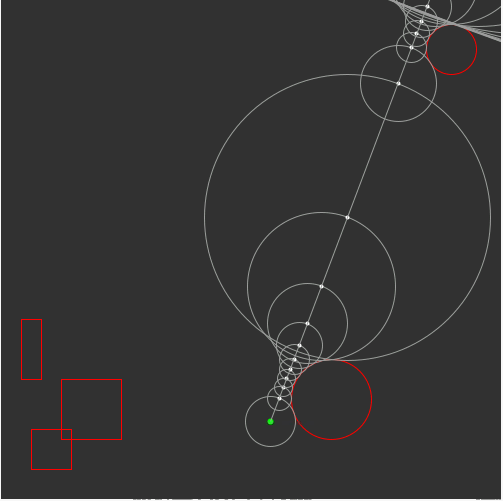
\includegraphics[width=8cm]{images/marching.png}
\begin{figure}[h]
    \centering
    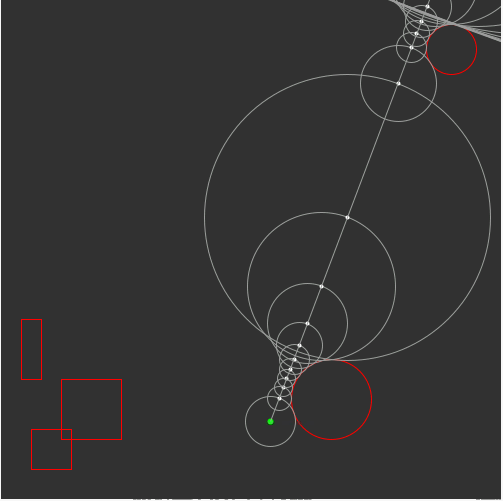
\includegraphics[width=8cm]{images/marching.png}
    \caption{Illustration 2D de la marche point par point d'un rayon (plus de details dans \ref{subsec:projection} \nameref{subsec:projection})}
    \label{fig:my_label}
\end{figure}

\clearpage
\documentclass[a4paper,11pt,twoside]{article} 
%\documentclass{article}


\author{Victor LASSERRE \& Valentin SERVIERES}
\pdfminorversion=7 % To use charte graphique (pdf 1.7)
\usepackage[utf8]{inputenc}
\usepackage[T1]{fontenc}
\usepackage{lscape}
\usepackage{boldline,multirow,tabularx,colortbl,makecell,fancybox,amsfonts,amssymb,amsmath,mathrsfs,array, svg}
\usepackage{pgf,tikz,xcolor,graphicx}
\usetikzlibrary{calc,positioning,shapes.geometric,shapes.symbols,shapes.misc, fit, shapes, arrows, arrows.meta,fadings,through}
\usepackage[top=2cm, bottom=2cm, left=2cm, right=2cm]{geometry}
\usepackage{hyperref,titlesec,eurosym,eso-pic,float}
\usepackage[french]{babel}
%\usepackage{bibleref} ajouté par moi mais flemme
% minted et les encars de code en gros
%\usepackage[newfloat]{minted}
\usepackage{caption}
\usepackage{tcolorbox}
%\newenvironment{code}{\captionsetup{type=listing}}{}
%\SetupFloatingEnvironment{listing}{name=Code Source}

% table des annexes
\usepackage{minitoc}
\usepackage{pdfpages}

% bibliographie
%\usepackage{biblatex}
%\usepackage{csquotes}
%\addbibresource{bibliography.bib}

%\input{advanced.params/listings.conf}
\input{charteINSA/advanced.params/tikz.conf}
\input{charteINSA/advanced.params/misc.commands}
\input{charteINSA/cover/covermain.tex}



%\usepackage[french]{babel}

% resolve no citation problem
\nocite{*}
%\usepackage[...,backend=bibtex]{biblatex}

% Set page size and margins
% Replace `letterpaper' with `a4paper' for UK/EU standard size
%%%%%\usepackage[letterpaper,top=2cm,bottom=2cm,left=3cm,right=3cm,marginparwidth=1.75cm]{geometry}

% Useful packages
\usepackage{listings}

\input{preferences/listings-glsl.prf}
% optionally set GLSL as default language
\lstset{language=GLSL}
\lstset{
  breaklines=true,
  breakatwhitespace=true,
  numbers=left,
  basicstyle={\small\ttfamily},
  numberstyle=\tiny\color{gray},
  tabsize=3,% end normal settings
  breaklines=true,                              % break long lines
  commentstyle=\itshape\color{green},           % comments are green
  keywordstyle=[1]\color{blue},                 % instructions are blue
  keywordstyle=[2]\color{orange},               % sections/other directives are orange
  keywordstyle=[3]\color{red},                   % registers are red
  stringstyle=\color{mauve},                    % strings are from the telekom
  identifierstyle=\color{teal},                 % user declared addresses are teal
  frame=l,                                      % black line on the left side of code
  language=GLSL,                   % all code is RISC-V
  tabsize=4,                                    % indent tabs with 4 spaces
  showstringspaces=false                        % do not replace spaces with weird underlines
}

\usepackage[square,numbers]{natbib}
\bibliographystyle{abbrvnat}
%Includes "References" in the table of contents
\usepackage[nottoc]{tocbibind}

\usepackage{setspace}
\usepackage{titletoc}
%\usepackage[T1]{fontenc}
%\usepackage{amsfonts}
%\usepackage{graphicx}
\usepackage{mathtools}
\graphicspath{ {images/} }

%\usepackage{fancyhdr}
\pagestyle{fancy}
\renewcommand\headrulewidth{1pt}
\fancyhead[L]{\textsf{Moteur graphique}}
\fancyhead[R]{\textsf{}}
%\usepackage[colorlinks=true, allcolors=blue]{hyperref}


\begin{document}
\dosecttoc{} % generate TOC
%\maketitle
\clearpage

% Remerciements
\thispagestyle{empty} % removes page number
\subsection*{Remerciements}
Nous tenons à remercier notre tuteur de projet M. Sanchez, notamment pour son aide précieuse et ses conseils. \\
Nous remercions également Inigo Quilez pour la riche documentation sur le ray marching qu'il fournit librement sur son site web.
\clearpage

% TABLE DES MATIÈRES
\thispagestyle{empty} % removes page number
\setcounter{secnumdepth}{3}
\tableofcontents
\clearpage

\setcounter{page}{1}


\sectionnn{Introduction}

    Engin Pas Tangible est un moteur graphique reposant sur le principe de Ray Marching : un système de 3D similaire au Ray Tracing, mais beaucoup plus rarement utilisé. Ce système a certains avantages par rapport au Ray Tracing, comme par exemple de permettre une implémetation peu coûteuse de fractales, ou autres figures se reproduisant à l'identique. \\
    Le Ray Marching repose sur la projection de rayons depuis une camera vers la scene. Pour projeter un rayon, on le fait avancer pas à pas (\emph{Marching}). La distance des pas doit être la plus grande possible, mais sans que le rayon ne traverse d'objet de la scene 3D.
\\
\\
%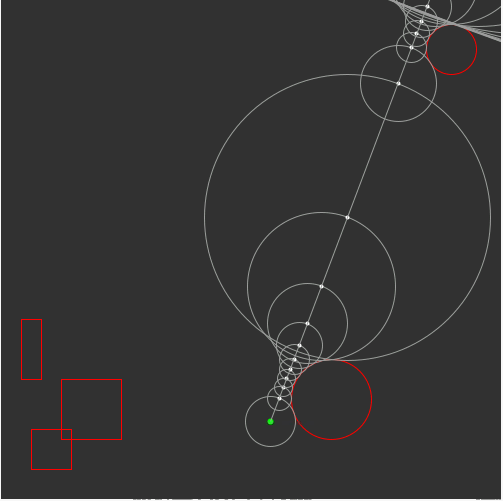
\includegraphics[width=8cm]{images/marching.png}
\begin{figure}[h]
    \centering
    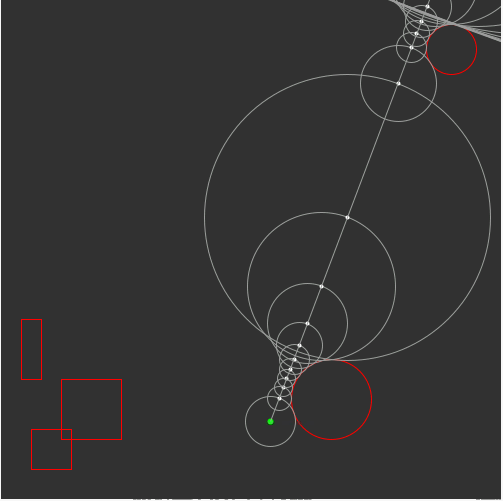
\includegraphics[width=8cm]{images/marching.png}
    \caption{Illustration 2D de la marche point par point d'un rayon (plus de details dans \ref{subsec:projection} \nameref{subsec:projection})}
    \label{fig:my_label}
\end{figure}

\clearpage
\documentclass[a4paper,11pt,twoside]{article} 
%\documentclass{article}

\input{charteINSA/maincharte.tex}

%\usepackage[french]{babel}

% resolve no citation problem
\nocite{*}
%\usepackage[...,backend=bibtex]{biblatex}

% Set page size and margins
% Replace `letterpaper' with `a4paper' for UK/EU standard size
%%%%%\usepackage[letterpaper,top=2cm,bottom=2cm,left=3cm,right=3cm,marginparwidth=1.75cm]{geometry}

% Useful packages
\usepackage{listings}

\input{preferences/listings-glsl.prf}
% optionally set GLSL as default language
\lstset{language=GLSL}
\input{preferences/glsl.tex}

\usepackage[square,numbers]{natbib}
\bibliographystyle{abbrvnat}
%Includes "References" in the table of contents
\usepackage[nottoc]{tocbibind}

\usepackage{setspace}
\usepackage{titletoc}
%\usepackage[T1]{fontenc}
%\usepackage{amsfonts}
%\usepackage{graphicx}
\usepackage{mathtools}
\graphicspath{ {images/} }

%\input{hautdepage.tex}
%\usepackage[colorlinks=true, allcolors=blue]{hyperref}


\begin{document}
\dosecttoc{} % generate TOC
%\maketitle
\clearpage

% Remerciements
\thispagestyle{empty} % removes page number
\subsection*{Remerciements}
Nous tenons à remercier notre tuteur de projet M. Sanchez, notamment pour son aide précieuse et ses conseils. \\
Nous remercions également Inigo Quilez pour la riche documentation sur le ray marching qu'il fournit librement sur son site web.
\clearpage

% TABLE DES MATIÈRES
\thispagestyle{empty} % removes page number
\setcounter{secnumdepth}{3}
\tableofcontents
\clearpage

\setcounter{page}{1}


\input{Parties/Introduction}
\clearpage
\input{Parties/Fonctionnement/main}
\clearpage
\input{Parties/Fonctionnalites/main}
\clearpage
\input{Parties/Historique/main}
\clearpage
\input{Parties/Conclusion}

\clearpage


%Imports the bibliography file "sample.bib"
\bibliography{sample}
\clearpage

% TABLE DES ANNEXES
\clearpage
\appendix
%\thispagestyle{empty} % removes page number
\sectionnn{Table des Annexes}
\addtocontents{toc}{\protect\setcounter{tocdepth}{0}}
\renewcommand{\stctitle}{}                          % Titre (issue with previous subsection showing up)
\renewcommand\thesubsection{A\arabic{subsection}}   % Numérotation
\renewcommand{\stcSSfont}{}                         % Police normale, pas en gras
\mtcsetrules{secttoc}{off}                          % Désactivation des lignes en haut et en bas de la table

% Affichage de la table des annexes
\secttoc
% ANNEXES
\clearpage
\pagenumbering{Roman}


\input{Parties/Annexes}

\mtcsetrules{secttoc}{off}

\end{document}


                        

\clearpage
\documentclass[a4paper,11pt,twoside]{article} 
%\documentclass{article}

\input{charteINSA/maincharte.tex}

%\usepackage[french]{babel}

% resolve no citation problem
\nocite{*}
%\usepackage[...,backend=bibtex]{biblatex}

% Set page size and margins
% Replace `letterpaper' with `a4paper' for UK/EU standard size
%%%%%\usepackage[letterpaper,top=2cm,bottom=2cm,left=3cm,right=3cm,marginparwidth=1.75cm]{geometry}

% Useful packages
\usepackage{listings}

\input{preferences/listings-glsl.prf}
% optionally set GLSL as default language
\lstset{language=GLSL}
\input{preferences/glsl.tex}

\usepackage[square,numbers]{natbib}
\bibliographystyle{abbrvnat}
%Includes "References" in the table of contents
\usepackage[nottoc]{tocbibind}

\usepackage{setspace}
\usepackage{titletoc}
%\usepackage[T1]{fontenc}
%\usepackage{amsfonts}
%\usepackage{graphicx}
\usepackage{mathtools}
\graphicspath{ {images/} }

%\input{hautdepage.tex}
%\usepackage[colorlinks=true, allcolors=blue]{hyperref}


\begin{document}
\dosecttoc{} % generate TOC
%\maketitle
\clearpage

% Remerciements
\thispagestyle{empty} % removes page number
\subsection*{Remerciements}
Nous tenons à remercier notre tuteur de projet M. Sanchez, notamment pour son aide précieuse et ses conseils. \\
Nous remercions également Inigo Quilez pour la riche documentation sur le ray marching qu'il fournit librement sur son site web.
\clearpage

% TABLE DES MATIÈRES
\thispagestyle{empty} % removes page number
\setcounter{secnumdepth}{3}
\tableofcontents
\clearpage

\setcounter{page}{1}


\input{Parties/Introduction}
\clearpage
\input{Parties/Fonctionnement/main}
\clearpage
\input{Parties/Fonctionnalites/main}
\clearpage
\input{Parties/Historique/main}
\clearpage
\input{Parties/Conclusion}

\clearpage


%Imports the bibliography file "sample.bib"
\bibliography{sample}
\clearpage

% TABLE DES ANNEXES
\clearpage
\appendix
%\thispagestyle{empty} % removes page number
\sectionnn{Table des Annexes}
\addtocontents{toc}{\protect\setcounter{tocdepth}{0}}
\renewcommand{\stctitle}{}                          % Titre (issue with previous subsection showing up)
\renewcommand\thesubsection{A\arabic{subsection}}   % Numérotation
\renewcommand{\stcSSfont}{}                         % Police normale, pas en gras
\mtcsetrules{secttoc}{off}                          % Désactivation des lignes en haut et en bas de la table

% Affichage de la table des annexes
\secttoc
% ANNEXES
\clearpage
\pagenumbering{Roman}


\input{Parties/Annexes}

\mtcsetrules{secttoc}{off}

\end{document}


                        

\clearpage
\documentclass[a4paper,11pt,twoside]{article} 
%\documentclass{article}

\input{charteINSA/maincharte.tex}

%\usepackage[french]{babel}

% resolve no citation problem
\nocite{*}
%\usepackage[...,backend=bibtex]{biblatex}

% Set page size and margins
% Replace `letterpaper' with `a4paper' for UK/EU standard size
%%%%%\usepackage[letterpaper,top=2cm,bottom=2cm,left=3cm,right=3cm,marginparwidth=1.75cm]{geometry}

% Useful packages
\usepackage{listings}

\input{preferences/listings-glsl.prf}
% optionally set GLSL as default language
\lstset{language=GLSL}
\input{preferences/glsl.tex}

\usepackage[square,numbers]{natbib}
\bibliographystyle{abbrvnat}
%Includes "References" in the table of contents
\usepackage[nottoc]{tocbibind}

\usepackage{setspace}
\usepackage{titletoc}
%\usepackage[T1]{fontenc}
%\usepackage{amsfonts}
%\usepackage{graphicx}
\usepackage{mathtools}
\graphicspath{ {images/} }

%\input{hautdepage.tex}
%\usepackage[colorlinks=true, allcolors=blue]{hyperref}


\begin{document}
\dosecttoc{} % generate TOC
%\maketitle
\clearpage

% Remerciements
\thispagestyle{empty} % removes page number
\subsection*{Remerciements}
Nous tenons à remercier notre tuteur de projet M. Sanchez, notamment pour son aide précieuse et ses conseils. \\
Nous remercions également Inigo Quilez pour la riche documentation sur le ray marching qu'il fournit librement sur son site web.
\clearpage

% TABLE DES MATIÈRES
\thispagestyle{empty} % removes page number
\setcounter{secnumdepth}{3}
\tableofcontents
\clearpage

\setcounter{page}{1}


\input{Parties/Introduction}
\clearpage
\input{Parties/Fonctionnement/main}
\clearpage
\input{Parties/Fonctionnalites/main}
\clearpage
\input{Parties/Historique/main}
\clearpage
\input{Parties/Conclusion}

\clearpage


%Imports the bibliography file "sample.bib"
\bibliography{sample}
\clearpage

% TABLE DES ANNEXES
\clearpage
\appendix
%\thispagestyle{empty} % removes page number
\sectionnn{Table des Annexes}
\addtocontents{toc}{\protect\setcounter{tocdepth}{0}}
\renewcommand{\stctitle}{}                          % Titre (issue with previous subsection showing up)
\renewcommand\thesubsection{A\arabic{subsection}}   % Numérotation
\renewcommand{\stcSSfont}{}                         % Police normale, pas en gras
\mtcsetrules{secttoc}{off}                          % Désactivation des lignes en haut et en bas de la table

% Affichage de la table des annexes
\secttoc
% ANNEXES
\clearpage
\pagenumbering{Roman}


\input{Parties/Annexes}

\mtcsetrules{secttoc}{off}

\end{document}


                        

\clearpage
\sectionnn{Conclusion}

Ce projet a été captivant et très motivant. Le fait de pouvoir observer rapidement les résultats de notre code était très agréable.\\
Nous avons rempli et même dépassé les objectifs que nous nous étions fixés.\\
Il était également intéressant de retrouver des notions vues en maths à l'INSA dans une application concrète.\\ \par

L'expérience fut très enrichissante car nous avons dû nous organiser pour pouvoir travailler en binôme sur le même code avec l'utilisation d'un gestionnaire de version (git) auquel nous nous sommes formés.\\
Nous avons pu explorer le principe du Ray Marching, découvrir un nouveau langage, le GLSL, ainsi que les bases de développement logiciel.\\ \par

Ce rapport était également l'occasion d'apprendre à maîtriser le LaTeX, mais c'était surtout l'occasion d'expliquer de façon claire et concise un concept technique.\\ \par

Finalement, ce projet de moteur graphique nous a beaucoup apporté et nous pensons continuer à le développer dans le futur.

\clearpage


%Imports the bibliography file "sample.bib"
\bibliography{sample}
\clearpage

% TABLE DES ANNEXES
\clearpage
\appendix
%\thispagestyle{empty} % removes page number
\sectionnn{Table des Annexes}
\addtocontents{toc}{\protect\setcounter{tocdepth}{0}}
\renewcommand{\stctitle}{}                          % Titre (issue with previous subsection showing up)
\renewcommand\thesubsection{A\arabic{subsection}}   % Numérotation
\renewcommand{\stcSSfont}{}                         % Police normale, pas en gras
\mtcsetrules{secttoc}{off}                          % Désactivation des lignes en haut et en bas de la table

% Affichage de la table des annexes
\secttoc
% ANNEXES
\clearpage
\pagenumbering{Roman}


\subsection{Scène simple}
%\addcontentsline{toc}{section}{Scène simple}
Code à mettre dans un fichier, nommé \emph{example.fs} par exemple
\begin{lstlisting}[language=GLSL]
#version 330 core
in vec2 FragCoord;
in float Time;
in vec2 MousePos;
in vec3 CamPos;
in vec3 CamDir;

out vec4 FragColor;
//uniform sampler2D generalTexture;

float SDF_Box_Frame( vec3 p, vec3 b, float e )
{
       p = abs(p  )-b;
  vec3 q = abs(p+e)-e;
  return min(min(
      length(max(vec3(p.x,q.y,q.z),0.0))+min(max(p.x,max(q.y,q.z)),0.0),
      length(max(vec3(q.x,p.y,q.z),0.0))+min(max(q.x,max(p.y,q.z)),0.0)),
      length(max(vec3(q.x,q.y,p.z),0.0))+min(max(q.x,max(q.y,p.z)),0.0));
}

float SDF_Circle(vec3 p,float r){
    return length(p)-r;
}

float SDF_Global(vec3 p){
    return min(
        SDF_Box_Frame(p,vec3(.5,.5,.5),0.1),
        SDF_Circle(mod(p+vec3(.5),vec3(1.,1.,1.))-vec3(.5),.15));
}

vec4 Get_Impact(vec3 origin,vec3 dir){//must have length(dir)==1 
    vec3 pos=origin;
    float dist;
    for(int i=0;i<30;i++){
        dist=SDF_Global(pos);
        pos+=dist*dir;
        if(dist<=.01) return vec4(pos,1.);
        if(dist>=20.0) return vec4(pos,-1.);
    }
    return vec4(pos,-1.);
}

vec3 grad(vec3 p){
    vec2 epsilon = vec2(.01,0.);
    return normalize(vec3(SDF_Global(p+epsilon.xyy)-SDF_Global(p-epsilon.xyy),
    SDF_Global(p+epsilon.yxy)-SDF_Global(p-epsilon.yxy),
    SDF_Global(p+epsilon.yyx)-SDF_Global(p-epsilon.yyx)));
}

vec3 Get_Color(vec3 origin,vec3 dir){
    vec4 impact = Get_Impact(origin,dir);
    if(impact.w<0.) return vec3(.5,.7,1.);
    vec3 normale=grad(impact.xyz);
    return normale;
}

void main()
{
    vec3 lookingAt = vec3(0.,0.,0.);
    vec3 posCam    = vec3(3.*sin(Time*.5),0.,3.*cos(Time*.5));
    
    vec3 ez = normalize(lookingAt - posCam); //base orthonormee
    vec3 ex = normalize(cross(ez,vec3(0.,1.,0.)));
    vec3 ey = cross(ex,ez);
    
    vec3 dir = normalize(FragCoord.x * ex + FragCoord.y*ey + 1.*ez);
    
  FragColor=vec4(Get_Color(posCam,dir),1.);
}
\end{lstlisting}

\mtcsetrules{secttoc}{off}

\end{document}


                        

\clearpage
\documentclass[a4paper,11pt,twoside]{article} 
%\documentclass{article}


\author{Victor LASSERRE \& Valentin SERVIERES}
\pdfminorversion=7 % To use charte graphique (pdf 1.7)
\usepackage[utf8]{inputenc}
\usepackage[T1]{fontenc}
\usepackage{lscape}
\usepackage{boldline,multirow,tabularx,colortbl,makecell,fancybox,amsfonts,amssymb,amsmath,mathrsfs,array, svg}
\usepackage{pgf,tikz,xcolor,graphicx}
\usetikzlibrary{calc,positioning,shapes.geometric,shapes.symbols,shapes.misc, fit, shapes, arrows, arrows.meta,fadings,through}
\usepackage[top=2cm, bottom=2cm, left=2cm, right=2cm]{geometry}
\usepackage{hyperref,titlesec,eurosym,eso-pic,float}
\usepackage[french]{babel}
%\usepackage{bibleref} ajouté par moi mais flemme
% minted et les encars de code en gros
%\usepackage[newfloat]{minted}
\usepackage{caption}
\usepackage{tcolorbox}
%\newenvironment{code}{\captionsetup{type=listing}}{}
%\SetupFloatingEnvironment{listing}{name=Code Source}

% table des annexes
\usepackage{minitoc}
\usepackage{pdfpages}

% bibliographie
%\usepackage{biblatex}
%\usepackage{csquotes}
%\addbibresource{bibliography.bib}

%\input{advanced.params/listings.conf}
\input{charteINSA/advanced.params/tikz.conf}
\input{charteINSA/advanced.params/misc.commands}
\input{charteINSA/cover/covermain.tex}



%\usepackage[french]{babel}

% resolve no citation problem
\nocite{*}
%\usepackage[...,backend=bibtex]{biblatex}

% Set page size and margins
% Replace `letterpaper' with `a4paper' for UK/EU standard size
%%%%%\usepackage[letterpaper,top=2cm,bottom=2cm,left=3cm,right=3cm,marginparwidth=1.75cm]{geometry}

% Useful packages
\usepackage{listings}

\input{preferences/listings-glsl.prf}
% optionally set GLSL as default language
\lstset{language=GLSL}
\lstset{
  breaklines=true,
  breakatwhitespace=true,
  numbers=left,
  basicstyle={\small\ttfamily},
  numberstyle=\tiny\color{gray},
  tabsize=3,% end normal settings
  breaklines=true,                              % break long lines
  commentstyle=\itshape\color{green},           % comments are green
  keywordstyle=[1]\color{blue},                 % instructions are blue
  keywordstyle=[2]\color{orange},               % sections/other directives are orange
  keywordstyle=[3]\color{red},                   % registers are red
  stringstyle=\color{mauve},                    % strings are from the telekom
  identifierstyle=\color{teal},                 % user declared addresses are teal
  frame=l,                                      % black line on the left side of code
  language=GLSL,                   % all code is RISC-V
  tabsize=4,                                    % indent tabs with 4 spaces
  showstringspaces=false                        % do not replace spaces with weird underlines
}

\usepackage[square,numbers]{natbib}
\bibliographystyle{abbrvnat}
%Includes "References" in the table of contents
\usepackage[nottoc]{tocbibind}

\usepackage{setspace}
\usepackage{titletoc}
%\usepackage[T1]{fontenc}
%\usepackage{amsfonts}
%\usepackage{graphicx}
\usepackage{mathtools}
\graphicspath{ {images/} }

%\usepackage{fancyhdr}
\pagestyle{fancy}
\renewcommand\headrulewidth{1pt}
\fancyhead[L]{\textsf{Moteur graphique}}
\fancyhead[R]{\textsf{}}
%\usepackage[colorlinks=true, allcolors=blue]{hyperref}


\begin{document}
\dosecttoc{} % generate TOC
%\maketitle
\clearpage

% Remerciements
\thispagestyle{empty} % removes page number
\subsection*{Remerciements}
Nous tenons à remercier notre tuteur de projet M. Sanchez, notamment pour son aide précieuse et ses conseils. \\
Nous remercions également Inigo Quilez pour la riche documentation sur le ray marching qu'il fournit librement sur son site web.
\clearpage

% TABLE DES MATIÈRES
\thispagestyle{empty} % removes page number
\setcounter{secnumdepth}{3}
\tableofcontents
\clearpage

\setcounter{page}{1}


\sectionnn{Introduction}

    Engin Pas Tangible est un moteur graphique reposant sur le principe de Ray Marching : un système de 3D similaire au Ray Tracing, mais beaucoup plus rarement utilisé. Ce système a certains avantages par rapport au Ray Tracing, comme par exemple de permettre une implémetation peu coûteuse de fractales, ou autres figures se reproduisant à l'identique. \\
    Le Ray Marching repose sur la projection de rayons depuis une camera vers la scene. Pour projeter un rayon, on le fait avancer pas à pas (\emph{Marching}). La distance des pas doit être la plus grande possible, mais sans que le rayon ne traverse d'objet de la scene 3D.
\\
\\
%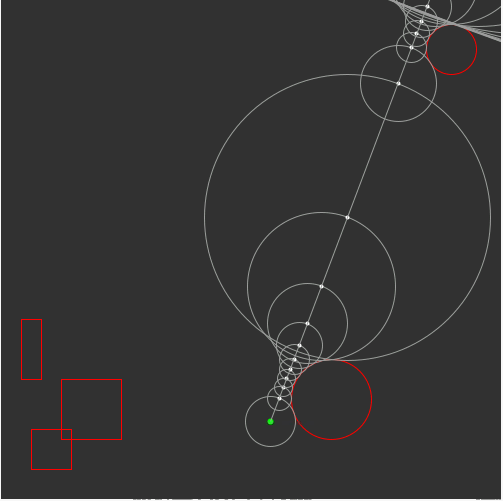
\includegraphics[width=8cm]{images/marching.png}
\begin{figure}[h]
    \centering
    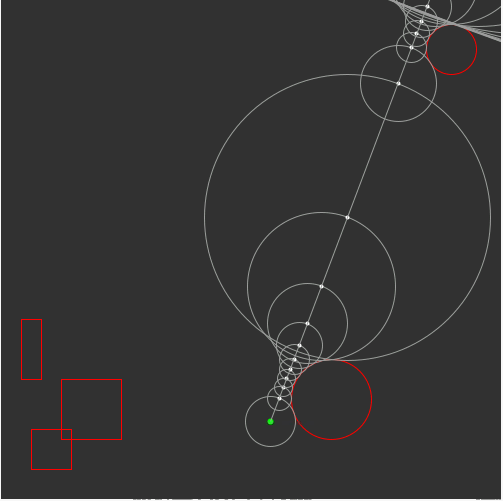
\includegraphics[width=8cm]{images/marching.png}
    \caption{Illustration 2D de la marche point par point d'un rayon (plus de details dans \ref{subsec:projection} \nameref{subsec:projection})}
    \label{fig:my_label}
\end{figure}

\clearpage
\documentclass[a4paper,11pt,twoside]{article} 
%\documentclass{article}

\input{charteINSA/maincharte.tex}

%\usepackage[french]{babel}

% resolve no citation problem
\nocite{*}
%\usepackage[...,backend=bibtex]{biblatex}

% Set page size and margins
% Replace `letterpaper' with `a4paper' for UK/EU standard size
%%%%%\usepackage[letterpaper,top=2cm,bottom=2cm,left=3cm,right=3cm,marginparwidth=1.75cm]{geometry}

% Useful packages
\usepackage{listings}

\input{preferences/listings-glsl.prf}
% optionally set GLSL as default language
\lstset{language=GLSL}
\input{preferences/glsl.tex}

\usepackage[square,numbers]{natbib}
\bibliographystyle{abbrvnat}
%Includes "References" in the table of contents
\usepackage[nottoc]{tocbibind}

\usepackage{setspace}
\usepackage{titletoc}
%\usepackage[T1]{fontenc}
%\usepackage{amsfonts}
%\usepackage{graphicx}
\usepackage{mathtools}
\graphicspath{ {images/} }

%\input{hautdepage.tex}
%\usepackage[colorlinks=true, allcolors=blue]{hyperref}


\begin{document}
\dosecttoc{} % generate TOC
%\maketitle
\clearpage

% Remerciements
\thispagestyle{empty} % removes page number
\subsection*{Remerciements}
Nous tenons à remercier notre tuteur de projet M. Sanchez, notamment pour son aide précieuse et ses conseils. \\
Nous remercions également Inigo Quilez pour la riche documentation sur le ray marching qu'il fournit librement sur son site web.
\clearpage

% TABLE DES MATIÈRES
\thispagestyle{empty} % removes page number
\setcounter{secnumdepth}{3}
\tableofcontents
\clearpage

\setcounter{page}{1}


\input{Parties/Introduction}
\clearpage
\input{Parties/Fonctionnement/main}
\clearpage
\input{Parties/Fonctionnalites/main}
\clearpage
\input{Parties/Historique/main}
\clearpage
\input{Parties/Conclusion}

\clearpage


%Imports the bibliography file "sample.bib"
\bibliography{sample}
\clearpage

% TABLE DES ANNEXES
\clearpage
\appendix
%\thispagestyle{empty} % removes page number
\sectionnn{Table des Annexes}
\addtocontents{toc}{\protect\setcounter{tocdepth}{0}}
\renewcommand{\stctitle}{}                          % Titre (issue with previous subsection showing up)
\renewcommand\thesubsection{A\arabic{subsection}}   % Numérotation
\renewcommand{\stcSSfont}{}                         % Police normale, pas en gras
\mtcsetrules{secttoc}{off}                          % Désactivation des lignes en haut et en bas de la table

% Affichage de la table des annexes
\secttoc
% ANNEXES
\clearpage
\pagenumbering{Roman}


\input{Parties/Annexes}

\mtcsetrules{secttoc}{off}

\end{document}


                        

\clearpage
\documentclass[a4paper,11pt,twoside]{article} 
%\documentclass{article}

\input{charteINSA/maincharte.tex}

%\usepackage[french]{babel}

% resolve no citation problem
\nocite{*}
%\usepackage[...,backend=bibtex]{biblatex}

% Set page size and margins
% Replace `letterpaper' with `a4paper' for UK/EU standard size
%%%%%\usepackage[letterpaper,top=2cm,bottom=2cm,left=3cm,right=3cm,marginparwidth=1.75cm]{geometry}

% Useful packages
\usepackage{listings}

\input{preferences/listings-glsl.prf}
% optionally set GLSL as default language
\lstset{language=GLSL}
\input{preferences/glsl.tex}

\usepackage[square,numbers]{natbib}
\bibliographystyle{abbrvnat}
%Includes "References" in the table of contents
\usepackage[nottoc]{tocbibind}

\usepackage{setspace}
\usepackage{titletoc}
%\usepackage[T1]{fontenc}
%\usepackage{amsfonts}
%\usepackage{graphicx}
\usepackage{mathtools}
\graphicspath{ {images/} }

%\input{hautdepage.tex}
%\usepackage[colorlinks=true, allcolors=blue]{hyperref}


\begin{document}
\dosecttoc{} % generate TOC
%\maketitle
\clearpage

% Remerciements
\thispagestyle{empty} % removes page number
\subsection*{Remerciements}
Nous tenons à remercier notre tuteur de projet M. Sanchez, notamment pour son aide précieuse et ses conseils. \\
Nous remercions également Inigo Quilez pour la riche documentation sur le ray marching qu'il fournit librement sur son site web.
\clearpage

% TABLE DES MATIÈRES
\thispagestyle{empty} % removes page number
\setcounter{secnumdepth}{3}
\tableofcontents
\clearpage

\setcounter{page}{1}


\input{Parties/Introduction}
\clearpage
\input{Parties/Fonctionnement/main}
\clearpage
\input{Parties/Fonctionnalites/main}
\clearpage
\input{Parties/Historique/main}
\clearpage
\input{Parties/Conclusion}

\clearpage


%Imports the bibliography file "sample.bib"
\bibliography{sample}
\clearpage

% TABLE DES ANNEXES
\clearpage
\appendix
%\thispagestyle{empty} % removes page number
\sectionnn{Table des Annexes}
\addtocontents{toc}{\protect\setcounter{tocdepth}{0}}
\renewcommand{\stctitle}{}                          % Titre (issue with previous subsection showing up)
\renewcommand\thesubsection{A\arabic{subsection}}   % Numérotation
\renewcommand{\stcSSfont}{}                         % Police normale, pas en gras
\mtcsetrules{secttoc}{off}                          % Désactivation des lignes en haut et en bas de la table

% Affichage de la table des annexes
\secttoc
% ANNEXES
\clearpage
\pagenumbering{Roman}


\input{Parties/Annexes}

\mtcsetrules{secttoc}{off}

\end{document}


                        

\clearpage
\documentclass[a4paper,11pt,twoside]{article} 
%\documentclass{article}

\input{charteINSA/maincharte.tex}

%\usepackage[french]{babel}

% resolve no citation problem
\nocite{*}
%\usepackage[...,backend=bibtex]{biblatex}

% Set page size and margins
% Replace `letterpaper' with `a4paper' for UK/EU standard size
%%%%%\usepackage[letterpaper,top=2cm,bottom=2cm,left=3cm,right=3cm,marginparwidth=1.75cm]{geometry}

% Useful packages
\usepackage{listings}

\input{preferences/listings-glsl.prf}
% optionally set GLSL as default language
\lstset{language=GLSL}
\input{preferences/glsl.tex}

\usepackage[square,numbers]{natbib}
\bibliographystyle{abbrvnat}
%Includes "References" in the table of contents
\usepackage[nottoc]{tocbibind}

\usepackage{setspace}
\usepackage{titletoc}
%\usepackage[T1]{fontenc}
%\usepackage{amsfonts}
%\usepackage{graphicx}
\usepackage{mathtools}
\graphicspath{ {images/} }

%\input{hautdepage.tex}
%\usepackage[colorlinks=true, allcolors=blue]{hyperref}


\begin{document}
\dosecttoc{} % generate TOC
%\maketitle
\clearpage

% Remerciements
\thispagestyle{empty} % removes page number
\subsection*{Remerciements}
Nous tenons à remercier notre tuteur de projet M. Sanchez, notamment pour son aide précieuse et ses conseils. \\
Nous remercions également Inigo Quilez pour la riche documentation sur le ray marching qu'il fournit librement sur son site web.
\clearpage

% TABLE DES MATIÈRES
\thispagestyle{empty} % removes page number
\setcounter{secnumdepth}{3}
\tableofcontents
\clearpage

\setcounter{page}{1}


\input{Parties/Introduction}
\clearpage
\input{Parties/Fonctionnement/main}
\clearpage
\input{Parties/Fonctionnalites/main}
\clearpage
\input{Parties/Historique/main}
\clearpage
\input{Parties/Conclusion}

\clearpage


%Imports the bibliography file "sample.bib"
\bibliography{sample}
\clearpage

% TABLE DES ANNEXES
\clearpage
\appendix
%\thispagestyle{empty} % removes page number
\sectionnn{Table des Annexes}
\addtocontents{toc}{\protect\setcounter{tocdepth}{0}}
\renewcommand{\stctitle}{}                          % Titre (issue with previous subsection showing up)
\renewcommand\thesubsection{A\arabic{subsection}}   % Numérotation
\renewcommand{\stcSSfont}{}                         % Police normale, pas en gras
\mtcsetrules{secttoc}{off}                          % Désactivation des lignes en haut et en bas de la table

% Affichage de la table des annexes
\secttoc
% ANNEXES
\clearpage
\pagenumbering{Roman}


\input{Parties/Annexes}

\mtcsetrules{secttoc}{off}

\end{document}


                        

\clearpage
\sectionnn{Conclusion}

Ce projet a été captivant et très motivant. Le fait de pouvoir observer rapidement les résultats de notre code était très agréable.\\
Nous avons rempli et même dépassé les objectifs que nous nous étions fixés.\\
Il était également intéressant de retrouver des notions vues en maths à l'INSA dans une application concrète.\\ \par

L'expérience fut très enrichissante car nous avons dû nous organiser pour pouvoir travailler en binôme sur le même code avec l'utilisation d'un gestionnaire de version (git) auquel nous nous sommes formés.\\
Nous avons pu explorer le principe du Ray Marching, découvrir un nouveau langage, le GLSL, ainsi que les bases de développement logiciel.\\ \par

Ce rapport était également l'occasion d'apprendre à maîtriser le LaTeX, mais c'était surtout l'occasion d'expliquer de façon claire et concise un concept technique.\\ \par

Finalement, ce projet de moteur graphique nous a beaucoup apporté et nous pensons continuer à le développer dans le futur.

\clearpage


%Imports the bibliography file "sample.bib"
\bibliography{sample}
\clearpage

% TABLE DES ANNEXES
\clearpage
\appendix
%\thispagestyle{empty} % removes page number
\sectionnn{Table des Annexes}
\addtocontents{toc}{\protect\setcounter{tocdepth}{0}}
\renewcommand{\stctitle}{}                          % Titre (issue with previous subsection showing up)
\renewcommand\thesubsection{A\arabic{subsection}}   % Numérotation
\renewcommand{\stcSSfont}{}                         % Police normale, pas en gras
\mtcsetrules{secttoc}{off}                          % Désactivation des lignes en haut et en bas de la table

% Affichage de la table des annexes
\secttoc
% ANNEXES
\clearpage
\pagenumbering{Roman}


\subsection{Scène simple}
%\addcontentsline{toc}{section}{Scène simple}
Code à mettre dans un fichier, nommé \emph{example.fs} par exemple
\begin{lstlisting}[language=GLSL]
#version 330 core
in vec2 FragCoord;
in float Time;
in vec2 MousePos;
in vec3 CamPos;
in vec3 CamDir;

out vec4 FragColor;
//uniform sampler2D generalTexture;

float SDF_Box_Frame( vec3 p, vec3 b, float e )
{
       p = abs(p  )-b;
  vec3 q = abs(p+e)-e;
  return min(min(
      length(max(vec3(p.x,q.y,q.z),0.0))+min(max(p.x,max(q.y,q.z)),0.0),
      length(max(vec3(q.x,p.y,q.z),0.0))+min(max(q.x,max(p.y,q.z)),0.0)),
      length(max(vec3(q.x,q.y,p.z),0.0))+min(max(q.x,max(q.y,p.z)),0.0));
}

float SDF_Circle(vec3 p,float r){
    return length(p)-r;
}

float SDF_Global(vec3 p){
    return min(
        SDF_Box_Frame(p,vec3(.5,.5,.5),0.1),
        SDF_Circle(mod(p+vec3(.5),vec3(1.,1.,1.))-vec3(.5),.15));
}

vec4 Get_Impact(vec3 origin,vec3 dir){//must have length(dir)==1 
    vec3 pos=origin;
    float dist;
    for(int i=0;i<30;i++){
        dist=SDF_Global(pos);
        pos+=dist*dir;
        if(dist<=.01) return vec4(pos,1.);
        if(dist>=20.0) return vec4(pos,-1.);
    }
    return vec4(pos,-1.);
}

vec3 grad(vec3 p){
    vec2 epsilon = vec2(.01,0.);
    return normalize(vec3(SDF_Global(p+epsilon.xyy)-SDF_Global(p-epsilon.xyy),
    SDF_Global(p+epsilon.yxy)-SDF_Global(p-epsilon.yxy),
    SDF_Global(p+epsilon.yyx)-SDF_Global(p-epsilon.yyx)));
}

vec3 Get_Color(vec3 origin,vec3 dir){
    vec4 impact = Get_Impact(origin,dir);
    if(impact.w<0.) return vec3(.5,.7,1.);
    vec3 normale=grad(impact.xyz);
    return normale;
}

void main()
{
    vec3 lookingAt = vec3(0.,0.,0.);
    vec3 posCam    = vec3(3.*sin(Time*.5),0.,3.*cos(Time*.5));
    
    vec3 ez = normalize(lookingAt - posCam); //base orthonormee
    vec3 ex = normalize(cross(ez,vec3(0.,1.,0.)));
    vec3 ey = cross(ex,ez);
    
    vec3 dir = normalize(FragCoord.x * ex + FragCoord.y*ey + 1.*ez);
    
  FragColor=vec4(Get_Color(posCam,dir),1.);
}
\end{lstlisting}

\mtcsetrules{secttoc}{off}

\end{document}


                        

\clearpage
\documentclass[a4paper,11pt,twoside]{article} 
%\documentclass{article}


\author{Victor LASSERRE \& Valentin SERVIERES}
\pdfminorversion=7 % To use charte graphique (pdf 1.7)
\usepackage[utf8]{inputenc}
\usepackage[T1]{fontenc}
\usepackage{lscape}
\usepackage{boldline,multirow,tabularx,colortbl,makecell,fancybox,amsfonts,amssymb,amsmath,mathrsfs,array, svg}
\usepackage{pgf,tikz,xcolor,graphicx}
\usetikzlibrary{calc,positioning,shapes.geometric,shapes.symbols,shapes.misc, fit, shapes, arrows, arrows.meta,fadings,through}
\usepackage[top=2cm, bottom=2cm, left=2cm, right=2cm]{geometry}
\usepackage{hyperref,titlesec,eurosym,eso-pic,float}
\usepackage[french]{babel}
%\usepackage{bibleref} ajouté par moi mais flemme
% minted et les encars de code en gros
%\usepackage[newfloat]{minted}
\usepackage{caption}
\usepackage{tcolorbox}
%\newenvironment{code}{\captionsetup{type=listing}}{}
%\SetupFloatingEnvironment{listing}{name=Code Source}

% table des annexes
\usepackage{minitoc}
\usepackage{pdfpages}

% bibliographie
%\usepackage{biblatex}
%\usepackage{csquotes}
%\addbibresource{bibliography.bib}

%\input{advanced.params/listings.conf}
\input{charteINSA/advanced.params/tikz.conf}
\input{charteINSA/advanced.params/misc.commands}
\input{charteINSA/cover/covermain.tex}



%\usepackage[french]{babel}

% resolve no citation problem
\nocite{*}
%\usepackage[...,backend=bibtex]{biblatex}

% Set page size and margins
% Replace `letterpaper' with `a4paper' for UK/EU standard size
%%%%%\usepackage[letterpaper,top=2cm,bottom=2cm,left=3cm,right=3cm,marginparwidth=1.75cm]{geometry}

% Useful packages
\usepackage{listings}

\input{preferences/listings-glsl.prf}
% optionally set GLSL as default language
\lstset{language=GLSL}
\lstset{
  breaklines=true,
  breakatwhitespace=true,
  numbers=left,
  basicstyle={\small\ttfamily},
  numberstyle=\tiny\color{gray},
  tabsize=3,% end normal settings
  breaklines=true,                              % break long lines
  commentstyle=\itshape\color{green},           % comments are green
  keywordstyle=[1]\color{blue},                 % instructions are blue
  keywordstyle=[2]\color{orange},               % sections/other directives are orange
  keywordstyle=[3]\color{red},                   % registers are red
  stringstyle=\color{mauve},                    % strings are from the telekom
  identifierstyle=\color{teal},                 % user declared addresses are teal
  frame=l,                                      % black line on the left side of code
  language=GLSL,                   % all code is RISC-V
  tabsize=4,                                    % indent tabs with 4 spaces
  showstringspaces=false                        % do not replace spaces with weird underlines
}

\usepackage[square,numbers]{natbib}
\bibliographystyle{abbrvnat}
%Includes "References" in the table of contents
\usepackage[nottoc]{tocbibind}

\usepackage{setspace}
\usepackage{titletoc}
%\usepackage[T1]{fontenc}
%\usepackage{amsfonts}
%\usepackage{graphicx}
\usepackage{mathtools}
\graphicspath{ {images/} }

%\usepackage{fancyhdr}
\pagestyle{fancy}
\renewcommand\headrulewidth{1pt}
\fancyhead[L]{\textsf{Moteur graphique}}
\fancyhead[R]{\textsf{}}
%\usepackage[colorlinks=true, allcolors=blue]{hyperref}


\begin{document}
\dosecttoc{} % generate TOC
%\maketitle
\clearpage

% Remerciements
\thispagestyle{empty} % removes page number
\subsection*{Remerciements}
Nous tenons à remercier notre tuteur de projet M. Sanchez, notamment pour son aide précieuse et ses conseils. \\
Nous remercions également Inigo Quilez pour la riche documentation sur le ray marching qu'il fournit librement sur son site web.
\clearpage

% TABLE DES MATIÈRES
\thispagestyle{empty} % removes page number
\setcounter{secnumdepth}{3}
\tableofcontents
\clearpage

\setcounter{page}{1}


\sectionnn{Introduction}

    Engin Pas Tangible est un moteur graphique reposant sur le principe de Ray Marching : un système de 3D similaire au Ray Tracing, mais beaucoup plus rarement utilisé. Ce système a certains avantages par rapport au Ray Tracing, comme par exemple de permettre une implémetation peu coûteuse de fractales, ou autres figures se reproduisant à l'identique. \\
    Le Ray Marching repose sur la projection de rayons depuis une camera vers la scene. Pour projeter un rayon, on le fait avancer pas à pas (\emph{Marching}). La distance des pas doit être la plus grande possible, mais sans que le rayon ne traverse d'objet de la scene 3D.
\\
\\
%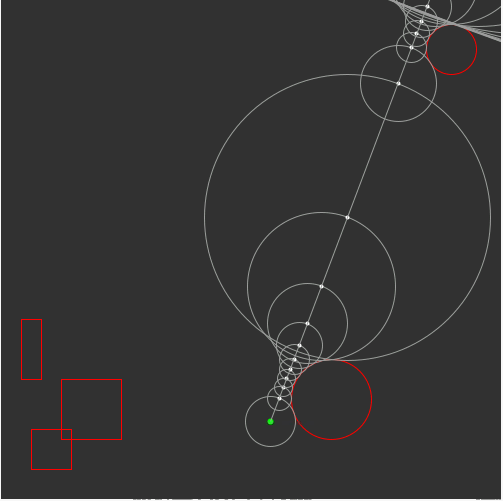
\includegraphics[width=8cm]{images/marching.png}
\begin{figure}[h]
    \centering
    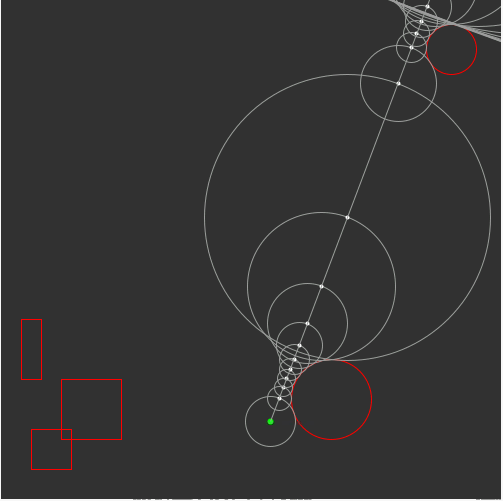
\includegraphics[width=8cm]{images/marching.png}
    \caption{Illustration 2D de la marche point par point d'un rayon (plus de details dans \ref{subsec:projection} \nameref{subsec:projection})}
    \label{fig:my_label}
\end{figure}

\clearpage
\documentclass[a4paper,11pt,twoside]{article} 
%\documentclass{article}

\input{charteINSA/maincharte.tex}

%\usepackage[french]{babel}

% resolve no citation problem
\nocite{*}
%\usepackage[...,backend=bibtex]{biblatex}

% Set page size and margins
% Replace `letterpaper' with `a4paper' for UK/EU standard size
%%%%%\usepackage[letterpaper,top=2cm,bottom=2cm,left=3cm,right=3cm,marginparwidth=1.75cm]{geometry}

% Useful packages
\usepackage{listings}

\input{preferences/listings-glsl.prf}
% optionally set GLSL as default language
\lstset{language=GLSL}
\input{preferences/glsl.tex}

\usepackage[square,numbers]{natbib}
\bibliographystyle{abbrvnat}
%Includes "References" in the table of contents
\usepackage[nottoc]{tocbibind}

\usepackage{setspace}
\usepackage{titletoc}
%\usepackage[T1]{fontenc}
%\usepackage{amsfonts}
%\usepackage{graphicx}
\usepackage{mathtools}
\graphicspath{ {images/} }

%\input{hautdepage.tex}
%\usepackage[colorlinks=true, allcolors=blue]{hyperref}


\begin{document}
\dosecttoc{} % generate TOC
%\maketitle
\clearpage

% Remerciements
\thispagestyle{empty} % removes page number
\subsection*{Remerciements}
Nous tenons à remercier notre tuteur de projet M. Sanchez, notamment pour son aide précieuse et ses conseils. \\
Nous remercions également Inigo Quilez pour la riche documentation sur le ray marching qu'il fournit librement sur son site web.
\clearpage

% TABLE DES MATIÈRES
\thispagestyle{empty} % removes page number
\setcounter{secnumdepth}{3}
\tableofcontents
\clearpage

\setcounter{page}{1}


\input{Parties/Introduction}
\clearpage
\input{Parties/Fonctionnement/main}
\clearpage
\input{Parties/Fonctionnalites/main}
\clearpage
\input{Parties/Historique/main}
\clearpage
\input{Parties/Conclusion}

\clearpage


%Imports the bibliography file "sample.bib"
\bibliography{sample}
\clearpage

% TABLE DES ANNEXES
\clearpage
\appendix
%\thispagestyle{empty} % removes page number
\sectionnn{Table des Annexes}
\addtocontents{toc}{\protect\setcounter{tocdepth}{0}}
\renewcommand{\stctitle}{}                          % Titre (issue with previous subsection showing up)
\renewcommand\thesubsection{A\arabic{subsection}}   % Numérotation
\renewcommand{\stcSSfont}{}                         % Police normale, pas en gras
\mtcsetrules{secttoc}{off}                          % Désactivation des lignes en haut et en bas de la table

% Affichage de la table des annexes
\secttoc
% ANNEXES
\clearpage
\pagenumbering{Roman}


\input{Parties/Annexes}

\mtcsetrules{secttoc}{off}

\end{document}


                        

\clearpage
\documentclass[a4paper,11pt,twoside]{article} 
%\documentclass{article}

\input{charteINSA/maincharte.tex}

%\usepackage[french]{babel}

% resolve no citation problem
\nocite{*}
%\usepackage[...,backend=bibtex]{biblatex}

% Set page size and margins
% Replace `letterpaper' with `a4paper' for UK/EU standard size
%%%%%\usepackage[letterpaper,top=2cm,bottom=2cm,left=3cm,right=3cm,marginparwidth=1.75cm]{geometry}

% Useful packages
\usepackage{listings}

\input{preferences/listings-glsl.prf}
% optionally set GLSL as default language
\lstset{language=GLSL}
\input{preferences/glsl.tex}

\usepackage[square,numbers]{natbib}
\bibliographystyle{abbrvnat}
%Includes "References" in the table of contents
\usepackage[nottoc]{tocbibind}

\usepackage{setspace}
\usepackage{titletoc}
%\usepackage[T1]{fontenc}
%\usepackage{amsfonts}
%\usepackage{graphicx}
\usepackage{mathtools}
\graphicspath{ {images/} }

%\input{hautdepage.tex}
%\usepackage[colorlinks=true, allcolors=blue]{hyperref}


\begin{document}
\dosecttoc{} % generate TOC
%\maketitle
\clearpage

% Remerciements
\thispagestyle{empty} % removes page number
\subsection*{Remerciements}
Nous tenons à remercier notre tuteur de projet M. Sanchez, notamment pour son aide précieuse et ses conseils. \\
Nous remercions également Inigo Quilez pour la riche documentation sur le ray marching qu'il fournit librement sur son site web.
\clearpage

% TABLE DES MATIÈRES
\thispagestyle{empty} % removes page number
\setcounter{secnumdepth}{3}
\tableofcontents
\clearpage

\setcounter{page}{1}


\input{Parties/Introduction}
\clearpage
\input{Parties/Fonctionnement/main}
\clearpage
\input{Parties/Fonctionnalites/main}
\clearpage
\input{Parties/Historique/main}
\clearpage
\input{Parties/Conclusion}

\clearpage


%Imports the bibliography file "sample.bib"
\bibliography{sample}
\clearpage

% TABLE DES ANNEXES
\clearpage
\appendix
%\thispagestyle{empty} % removes page number
\sectionnn{Table des Annexes}
\addtocontents{toc}{\protect\setcounter{tocdepth}{0}}
\renewcommand{\stctitle}{}                          % Titre (issue with previous subsection showing up)
\renewcommand\thesubsection{A\arabic{subsection}}   % Numérotation
\renewcommand{\stcSSfont}{}                         % Police normale, pas en gras
\mtcsetrules{secttoc}{off}                          % Désactivation des lignes en haut et en bas de la table

% Affichage de la table des annexes
\secttoc
% ANNEXES
\clearpage
\pagenumbering{Roman}


\input{Parties/Annexes}

\mtcsetrules{secttoc}{off}

\end{document}


                        

\clearpage
\documentclass[a4paper,11pt,twoside]{article} 
%\documentclass{article}

\input{charteINSA/maincharte.tex}

%\usepackage[french]{babel}

% resolve no citation problem
\nocite{*}
%\usepackage[...,backend=bibtex]{biblatex}

% Set page size and margins
% Replace `letterpaper' with `a4paper' for UK/EU standard size
%%%%%\usepackage[letterpaper,top=2cm,bottom=2cm,left=3cm,right=3cm,marginparwidth=1.75cm]{geometry}

% Useful packages
\usepackage{listings}

\input{preferences/listings-glsl.prf}
% optionally set GLSL as default language
\lstset{language=GLSL}
\input{preferences/glsl.tex}

\usepackage[square,numbers]{natbib}
\bibliographystyle{abbrvnat}
%Includes "References" in the table of contents
\usepackage[nottoc]{tocbibind}

\usepackage{setspace}
\usepackage{titletoc}
%\usepackage[T1]{fontenc}
%\usepackage{amsfonts}
%\usepackage{graphicx}
\usepackage{mathtools}
\graphicspath{ {images/} }

%\input{hautdepage.tex}
%\usepackage[colorlinks=true, allcolors=blue]{hyperref}


\begin{document}
\dosecttoc{} % generate TOC
%\maketitle
\clearpage

% Remerciements
\thispagestyle{empty} % removes page number
\subsection*{Remerciements}
Nous tenons à remercier notre tuteur de projet M. Sanchez, notamment pour son aide précieuse et ses conseils. \\
Nous remercions également Inigo Quilez pour la riche documentation sur le ray marching qu'il fournit librement sur son site web.
\clearpage

% TABLE DES MATIÈRES
\thispagestyle{empty} % removes page number
\setcounter{secnumdepth}{3}
\tableofcontents
\clearpage

\setcounter{page}{1}


\input{Parties/Introduction}
\clearpage
\input{Parties/Fonctionnement/main}
\clearpage
\input{Parties/Fonctionnalites/main}
\clearpage
\input{Parties/Historique/main}
\clearpage
\input{Parties/Conclusion}

\clearpage


%Imports the bibliography file "sample.bib"
\bibliography{sample}
\clearpage

% TABLE DES ANNEXES
\clearpage
\appendix
%\thispagestyle{empty} % removes page number
\sectionnn{Table des Annexes}
\addtocontents{toc}{\protect\setcounter{tocdepth}{0}}
\renewcommand{\stctitle}{}                          % Titre (issue with previous subsection showing up)
\renewcommand\thesubsection{A\arabic{subsection}}   % Numérotation
\renewcommand{\stcSSfont}{}                         % Police normale, pas en gras
\mtcsetrules{secttoc}{off}                          % Désactivation des lignes en haut et en bas de la table

% Affichage de la table des annexes
\secttoc
% ANNEXES
\clearpage
\pagenumbering{Roman}


\input{Parties/Annexes}

\mtcsetrules{secttoc}{off}

\end{document}


                        

\clearpage
\sectionnn{Conclusion}

Ce projet a été captivant et très motivant. Le fait de pouvoir observer rapidement les résultats de notre code était très agréable.\\
Nous avons rempli et même dépassé les objectifs que nous nous étions fixés.\\
Il était également intéressant de retrouver des notions vues en maths à l'INSA dans une application concrète.\\ \par

L'expérience fut très enrichissante car nous avons dû nous organiser pour pouvoir travailler en binôme sur le même code avec l'utilisation d'un gestionnaire de version (git) auquel nous nous sommes formés.\\
Nous avons pu explorer le principe du Ray Marching, découvrir un nouveau langage, le GLSL, ainsi que les bases de développement logiciel.\\ \par

Ce rapport était également l'occasion d'apprendre à maîtriser le LaTeX, mais c'était surtout l'occasion d'expliquer de façon claire et concise un concept technique.\\ \par

Finalement, ce projet de moteur graphique nous a beaucoup apporté et nous pensons continuer à le développer dans le futur.

\clearpage


%Imports the bibliography file "sample.bib"
\bibliography{sample}
\clearpage

% TABLE DES ANNEXES
\clearpage
\appendix
%\thispagestyle{empty} % removes page number
\sectionnn{Table des Annexes}
\addtocontents{toc}{\protect\setcounter{tocdepth}{0}}
\renewcommand{\stctitle}{}                          % Titre (issue with previous subsection showing up)
\renewcommand\thesubsection{A\arabic{subsection}}   % Numérotation
\renewcommand{\stcSSfont}{}                         % Police normale, pas en gras
\mtcsetrules{secttoc}{off}                          % Désactivation des lignes en haut et en bas de la table

% Affichage de la table des annexes
\secttoc
% ANNEXES
\clearpage
\pagenumbering{Roman}


\subsection{Scène simple}
%\addcontentsline{toc}{section}{Scène simple}
Code à mettre dans un fichier, nommé \emph{example.fs} par exemple
\begin{lstlisting}[language=GLSL]
#version 330 core
in vec2 FragCoord;
in float Time;
in vec2 MousePos;
in vec3 CamPos;
in vec3 CamDir;

out vec4 FragColor;
//uniform sampler2D generalTexture;

float SDF_Box_Frame( vec3 p, vec3 b, float e )
{
       p = abs(p  )-b;
  vec3 q = abs(p+e)-e;
  return min(min(
      length(max(vec3(p.x,q.y,q.z),0.0))+min(max(p.x,max(q.y,q.z)),0.0),
      length(max(vec3(q.x,p.y,q.z),0.0))+min(max(q.x,max(p.y,q.z)),0.0)),
      length(max(vec3(q.x,q.y,p.z),0.0))+min(max(q.x,max(q.y,p.z)),0.0));
}

float SDF_Circle(vec3 p,float r){
    return length(p)-r;
}

float SDF_Global(vec3 p){
    return min(
        SDF_Box_Frame(p,vec3(.5,.5,.5),0.1),
        SDF_Circle(mod(p+vec3(.5),vec3(1.,1.,1.))-vec3(.5),.15));
}

vec4 Get_Impact(vec3 origin,vec3 dir){//must have length(dir)==1 
    vec3 pos=origin;
    float dist;
    for(int i=0;i<30;i++){
        dist=SDF_Global(pos);
        pos+=dist*dir;
        if(dist<=.01) return vec4(pos,1.);
        if(dist>=20.0) return vec4(pos,-1.);
    }
    return vec4(pos,-1.);
}

vec3 grad(vec3 p){
    vec2 epsilon = vec2(.01,0.);
    return normalize(vec3(SDF_Global(p+epsilon.xyy)-SDF_Global(p-epsilon.xyy),
    SDF_Global(p+epsilon.yxy)-SDF_Global(p-epsilon.yxy),
    SDF_Global(p+epsilon.yyx)-SDF_Global(p-epsilon.yyx)));
}

vec3 Get_Color(vec3 origin,vec3 dir){
    vec4 impact = Get_Impact(origin,dir);
    if(impact.w<0.) return vec3(.5,.7,1.);
    vec3 normale=grad(impact.xyz);
    return normale;
}

void main()
{
    vec3 lookingAt = vec3(0.,0.,0.);
    vec3 posCam    = vec3(3.*sin(Time*.5),0.,3.*cos(Time*.5));
    
    vec3 ez = normalize(lookingAt - posCam); //base orthonormee
    vec3 ex = normalize(cross(ez,vec3(0.,1.,0.)));
    vec3 ey = cross(ex,ez);
    
    vec3 dir = normalize(FragCoord.x * ex + FragCoord.y*ey + 1.*ez);
    
  FragColor=vec4(Get_Color(posCam,dir),1.);
}
\end{lstlisting}

\mtcsetrules{secttoc}{off}

\end{document}


                        

\clearpage
\sectionnn{Conclusion}

Ce projet a été captivant et très motivant. Le fait de pouvoir observer rapidement les résultats de notre code était très agréable.\\
Nous avons rempli et même dépassé les objectifs que nous nous étions fixés.\\
Il était également intéressant de retrouver des notions vues en maths à l'INSA dans une application concrète.\\ \par

L'expérience fut très enrichissante car nous avons dû nous organiser pour pouvoir travailler en binôme sur le même code avec l'utilisation d'un gestionnaire de version (git) auquel nous nous sommes formés.\\
Nous avons pu explorer le principe du Ray Marching, découvrir un nouveau langage, le GLSL, ainsi que les bases de développement logiciel.\\ \par

Ce rapport était également l'occasion d'apprendre à maîtriser le LaTeX, mais c'était surtout l'occasion d'expliquer de façon claire et concise un concept technique.\\ \par

Finalement, ce projet de moteur graphique nous a beaucoup apporté et nous pensons continuer à le développer dans le futur.

\clearpage


%Imports the bibliography file "sample.bib"
\bibliography{sample}
\clearpage

% TABLE DES ANNEXES
\clearpage
\appendix
%\thispagestyle{empty} % removes page number
\sectionnn{Table des Annexes}
\addtocontents{toc}{\protect\setcounter{tocdepth}{0}}
\renewcommand{\stctitle}{}                          % Titre (issue with previous subsection showing up)
\renewcommand\thesubsection{A\arabic{subsection}}   % Numérotation
\renewcommand{\stcSSfont}{}                         % Police normale, pas en gras
\mtcsetrules{secttoc}{off}                          % Désactivation des lignes en haut et en bas de la table

% Affichage de la table des annexes
\secttoc
% ANNEXES
\clearpage
\pagenumbering{Roman}


\subsection{Scène simple}
%\addcontentsline{toc}{section}{Scène simple}
Code à mettre dans un fichier, nommé \emph{example.fs} par exemple
\begin{lstlisting}[language=GLSL]
#version 330 core
in vec2 FragCoord;
in float Time;
in vec2 MousePos;
in vec3 CamPos;
in vec3 CamDir;

out vec4 FragColor;
//uniform sampler2D generalTexture;

float SDF_Box_Frame( vec3 p, vec3 b, float e )
{
       p = abs(p  )-b;
  vec3 q = abs(p+e)-e;
  return min(min(
      length(max(vec3(p.x,q.y,q.z),0.0))+min(max(p.x,max(q.y,q.z)),0.0),
      length(max(vec3(q.x,p.y,q.z),0.0))+min(max(q.x,max(p.y,q.z)),0.0)),
      length(max(vec3(q.x,q.y,p.z),0.0))+min(max(q.x,max(q.y,p.z)),0.0));
}

float SDF_Circle(vec3 p,float r){
    return length(p)-r;
}

float SDF_Global(vec3 p){
    return min(
        SDF_Box_Frame(p,vec3(.5,.5,.5),0.1),
        SDF_Circle(mod(p+vec3(.5),vec3(1.,1.,1.))-vec3(.5),.15));
}

vec4 Get_Impact(vec3 origin,vec3 dir){//must have length(dir)==1 
    vec3 pos=origin;
    float dist;
    for(int i=0;i<30;i++){
        dist=SDF_Global(pos);
        pos+=dist*dir;
        if(dist<=.01) return vec4(pos,1.);
        if(dist>=20.0) return vec4(pos,-1.);
    }
    return vec4(pos,-1.);
}

vec3 grad(vec3 p){
    vec2 epsilon = vec2(.01,0.);
    return normalize(vec3(SDF_Global(p+epsilon.xyy)-SDF_Global(p-epsilon.xyy),
    SDF_Global(p+epsilon.yxy)-SDF_Global(p-epsilon.yxy),
    SDF_Global(p+epsilon.yyx)-SDF_Global(p-epsilon.yyx)));
}

vec3 Get_Color(vec3 origin,vec3 dir){
    vec4 impact = Get_Impact(origin,dir);
    if(impact.w<0.) return vec3(.5,.7,1.);
    vec3 normale=grad(impact.xyz);
    return normale;
}

void main()
{
    vec3 lookingAt = vec3(0.,0.,0.);
    vec3 posCam    = vec3(3.*sin(Time*.5),0.,3.*cos(Time*.5));
    
    vec3 ez = normalize(lookingAt - posCam); //base orthonormee
    vec3 ex = normalize(cross(ez,vec3(0.,1.,0.)));
    vec3 ey = cross(ex,ez);
    
    vec3 dir = normalize(FragCoord.x * ex + FragCoord.y*ey + 1.*ez);
    
  FragColor=vec4(Get_Color(posCam,dir),1.);
}
\end{lstlisting}

\mtcsetrules{secttoc}{off}

\end{document}


                        

\clearpage
\documentclass[a4paper,11pt,twoside]{article} 
%\documentclass{article}


\author{Victor LASSERRE \& Valentin SERVIERES}
\pdfminorversion=7 % To use charte graphique (pdf 1.7)
\usepackage[utf8]{inputenc}
\usepackage[T1]{fontenc}
\usepackage{lscape}
\usepackage{boldline,multirow,tabularx,colortbl,makecell,fancybox,amsfonts,amssymb,amsmath,mathrsfs,array, svg}
\usepackage{pgf,tikz,xcolor,graphicx}
\usetikzlibrary{calc,positioning,shapes.geometric,shapes.symbols,shapes.misc, fit, shapes, arrows, arrows.meta,fadings,through}
\usepackage[top=2cm, bottom=2cm, left=2cm, right=2cm]{geometry}
\usepackage{hyperref,titlesec,eurosym,eso-pic,float}
\usepackage[french]{babel}
%\usepackage{bibleref} ajouté par moi mais flemme
% minted et les encars de code en gros
%\usepackage[newfloat]{minted}
\usepackage{caption}
\usepackage{tcolorbox}
%\newenvironment{code}{\captionsetup{type=listing}}{}
%\SetupFloatingEnvironment{listing}{name=Code Source}

% table des annexes
\usepackage{minitoc}
\usepackage{pdfpages}

% bibliographie
%\usepackage{biblatex}
%\usepackage{csquotes}
%\addbibresource{bibliography.bib}

%%--------------------------------------------------------------%
%     This is the configuration file for package "listings"    %
%--------------------------------------------------------------%

%https://en.wikibooks.org/wiki/LaTeX/Source_Code_Listings

%\newcommand{\includecode}[2][c]{\lstinputlisting[language = #1, basicstyle=\ttfamily\bfseries]{#2}<!---->}


\definecolor{cgreen}{rgb}{0.596,0.765,0.475}
\definecolor{cgray}{rgb}{0.361,0.388,0.439}
\definecolor{cpurple}{rgb}{0.776,0.51,0.866}
\definecolor{cyellow}{rgb}{0.58,0,0.82}

\lstset{ 
  backgroundcolor = \color{white},   % choose the background color; you must add \usepackage{color} or \usepackage{xcolor}; should come as last argument
  basicstyle = \footnotesize,        % the size of the fonts that are used for the code
  breakatwhitespace = false,         % sets if automatic breaks should only happen at whitespace
  breaklines = true,                 % sets automatic line breaking
  captionpos = b,                    % sets the caption-position to bottom
  commentstyle = \color{cgray},      % comment style
  deletekeywords = {...},            % if you want to delete keywords from the given language
  escapeinside = {\%*}{*)},          % if you want to add LaTeX within your code
  extendedchars = true,              % lets you use non-ASCII characters; for 8-bits encodings only, does not work with UTF-8
  frame = single,	                   % adds a frame around the code
  keepspaces = true,                 % keeps spaces in text, useful for keeping indentation of code (possibly needs columns = flexible)
  keywordstyle = \color{blue},       % keyword style
  language = C,                     % the language of the code
  morekeywords = {*,...},            % if you want to add more keywords to the set
  numbers = left,                    % where to put the line-numbers; possible values are (none, left, right)
  numbersep = 5pt,                   % how far the line-numbers are from the code
  numberstyle = \tiny\color{black}, % the style that is used for the line-numbers
  rulecolor = \color{black},         % if not set, the frame-color may be changed on line-breaks within not-black text (e.g. comments (green here))
  showspaces = false,                % show spaces everywhere adding particular underscores; it overrides 'showstringspaces'
  showstringspaces = false,          % underline spaces within strings only
  showtabs = false,                  % show tabs within strings adding particular underscores
  stepnumber = 1,                    % the step between two line-numbers. If it's 1, each line will be numbered
  stringstyle = \color{cgreen},     % string literal style
  tabsize = 4,	                   % sets default tabsize to 2 spaces
  title = \lstname                   % show the filename of files included with \lstinputlisting; also try caption instead of title
}


\lstset{literate=
  {á}{{\'a}}1 {é}{{\'e}}1 {í}{{\'i}}1 {ó}{{\'o}}1 {ú}{{\'u}}1
  {Á}{{\'A}}1 {É}{{\'E}}1 {Í}{{\'I}}1 {Ó}{{\'O}}1 {Ú}{{\'U}}1
  {à}{{\`a}}1 {è}{{\`e}}1 {ì}{{\`i}}1 {ò}{{\`o}}1 {ù}{{\`u}}1
  {À}{{\`A}}1 {È}{{\'E}}1 {Ì}{{\`I}}1 {Ò}{{\`O}}1 {Ù}{{\`U}}1
  {ä}{{\"a}}1 {ë}{{\"e}}1 {ï}{{\"i}}1 {ö}{{\"o}}1 {ü}{{\"u}}1
  {Ä}{{\"A}}1 {Ë}{{\"E}}1 {Ï}{{\"I}}1 {Ö}{{\"O}}1 {Ü}{{\"U}}1
  {â}{{\^a}}1 {ê}{{\^e}}1 {î}{{\^i}}1 {ô}{{\^o}}1 {û}{{\^u}}1
  {Â}{{\^A}}1 {Ê}{{\^E}}1 {Î}{{\^I}}1 {Ô}{{\^O}}1 {Û}{{\^U}}1
  {œ}{{\oe}}1 {Œ}{{\OE}}1 {æ}{{\ae}}1 {Æ}{{\AE}}1 {ß}{{\ss}}1
  {ű}{{\H{u}}}1 {Ű}{{\H{U}}}1 {ő}{{\H{o}}}1 {Ő}{{\H{O}}}1
  {ç}{{\c c}}1 {Ç}{{\c C}}1 {ø}{{\o}}1 {å}{{\r a}}1 {Å}{{\r A}}1
  {€}{{\euro}}1 {£}{{\pounds}}1 {«}{{\guillemotleft}}1
  {»}{{\guillemotright}}1 {ñ}{{\~n}}1 {Ñ}{{\~N}}1 {¿}{{?`}}1
}

\tikzset{every picture/.style={execute at begin picture={
   \shorthandoff{:;!?};}
}}

\tikzset{
    boxnode/.style={ % requires library shapes.misc
        draw,
        rectangle,
        text centered,
        align=center,
        fill=gray!5!white
    },
}
\newcommand\tab[1][0.6cm]{\hspace*{#1}} %Create and define tab

\definecolor{lightgray}{gray}{0.85}
\definecolor{lightgrey}{gray}{0.85}
\definecolor{vlg}{gray}{0.85}


%Patch pour utiliser des équations dans les titres sans que hypperref nous insulte.
% Définition cyclique, compile pas. Mais c'est l"idée
%\renewcommand{\chapter}[1]{\chapter{\texorpdfstring{#1}}}
%\renewcommand{\section}[1]{\section{\texorpdfstring{#1}}}
%\renewcommand{\subsection}[1]{\subsection{\texorpdfstring{#1}}}
%\renewcommand{\subsubsection}[1]{\subsubsection{\texorpdfstring{#1}}}

%Chapter No Numbering but appears in TOC
\newcommand{\chapternn}[1]{\chapter*{#1}\addcontentsline{toc}{chapter}{#1}}
\newcommand{\sectionnn}[1]{\phantomsection\section*{#1}\addcontentsline{toc}{section}{#1}}
% phantomsection is necessary for links in TOC to function. It places the anchor
\newcommand{\subsectionnn}[1]{\subsection*{#1}\addcontentsline{toc}{subsection}{#1}}
\newcommand{\subsubsectionnn}[1]{\subsubsection*{#1}\addcontentsline{toc}{subsubsection}{#1}}

\newcolumntype{L}[1]{>{\raggedright\arraybackslash\hspace{0pt}}p{#1}}
\newcolumntype{R}[1]{>{\raggedleft\arraybackslash\hspace{0pt}}p{#1}}
\newcolumntype{C}[1]{>{\centering\arraybackslash\hspace{0pt}}p{#1}}


\renewcommand\thesection{\arabic{section}}
\renewcommand\thesubsection{\thesection.\arabic{subsection}}

%------- Do not append new commands after :

\hypersetup{	
    colorlinks=false, % colorise les liens
    linkbordercolor={1 1 1},
    breaklinks=true, % permet le retour à la ligne dans les liens trop longs
    urlcolor=blue, % couleur des hyperliens 
    linkcolor=black,	% couleur des liens internes 
    citecolor=black,	% couleur des références 
    pdftitle={}, % informations apparaissant dans 
    pdfauthor={}, % les informations du document
    pdfsubject={}	% sous Acrobat. 
}
\AtBeginDocument{\input{charteINSA/cover/cover_in.tex}\input{charteINSA/cover/cover_in_2.tex}\pagenumbering{arabic}}

%\AtEndDocument{\input{----cover/cover_out.tex}}




%\usepackage[french]{babel}

% resolve no citation problem
\nocite{*}
%\usepackage[...,backend=bibtex]{biblatex}

% Set page size and margins
% Replace `letterpaper' with `a4paper' for UK/EU standard size
%%%%%\usepackage[letterpaper,top=2cm,bottom=2cm,left=3cm,right=3cm,marginparwidth=1.75cm]{geometry}

% Useful packages
\usepackage{listings}

\input{preferences/listings-glsl.prf}
% optionally set GLSL as default language
\lstset{language=GLSL}
\lstset{
  breaklines=true,
  breakatwhitespace=true,
  numbers=left,
  basicstyle={\small\ttfamily},
  numberstyle=\tiny\color{gray},
  tabsize=3,% end normal settings
  breaklines=true,                              % break long lines
  commentstyle=\itshape\color{green},           % comments are green
  keywordstyle=[1]\color{blue},                 % instructions are blue
  keywordstyle=[2]\color{orange},               % sections/other directives are orange
  keywordstyle=[3]\color{red},                   % registers are red
  stringstyle=\color{mauve},                    % strings are from the telekom
  identifierstyle=\color{teal},                 % user declared addresses are teal
  frame=l,                                      % black line on the left side of code
  language=GLSL,                   % all code is RISC-V
  tabsize=4,                                    % indent tabs with 4 spaces
  showstringspaces=false                        % do not replace spaces with weird underlines
}

\usepackage[square,numbers]{natbib}
\bibliographystyle{abbrvnat}
%Includes "References" in the table of contents
\usepackage[nottoc]{tocbibind}

\usepackage{setspace}
\usepackage{titletoc}
%\usepackage[T1]{fontenc}
%\usepackage{amsfonts}
%\usepackage{graphicx}
\usepackage{mathtools}
\graphicspath{ {images/} }

%\usepackage{fancyhdr}
\pagestyle{fancy}
\renewcommand\headrulewidth{1pt}
\fancyhead[L]{\textsf{Moteur graphique}}
\fancyhead[R]{\textsf{}}
%\usepackage[colorlinks=true, allcolors=blue]{hyperref}


\begin{document}
\dosecttoc{} % generate TOC
%\maketitle
\clearpage

% Remerciements
\thispagestyle{empty} % removes page number
\subsection*{Remerciements}
Nous tenons à remercier notre tuteur de projet M. Sanchez, notamment pour son aide précieuse et ses conseils. \\
Nous remercions également Inigo Quilez pour la riche documentation sur le ray marching qu'il fournit librement sur son site web.
\clearpage

% TABLE DES MATIÈRES
\thispagestyle{empty} % removes page number
\setcounter{secnumdepth}{3}
\tableofcontents
\clearpage

\setcounter{page}{1}


\sectionnn{Introduction}

    Engin Pas Tangible est un moteur graphique reposant sur le principe de Ray Marching : un système de 3D similaire au Ray Tracing, mais beaucoup plus rarement utilisé. Ce système a certains avantages par rapport au Ray Tracing, comme par exemple de permettre une implémetation peu coûteuse de fractales, ou autres figures se reproduisant à l'identique. \\
    Le Ray Marching repose sur la projection de rayons depuis une camera vers la scene. Pour projeter un rayon, on le fait avancer pas à pas (\emph{Marching}). La distance des pas doit être la plus grande possible, mais sans que le rayon ne traverse d'objet de la scene 3D.
\\
\\
%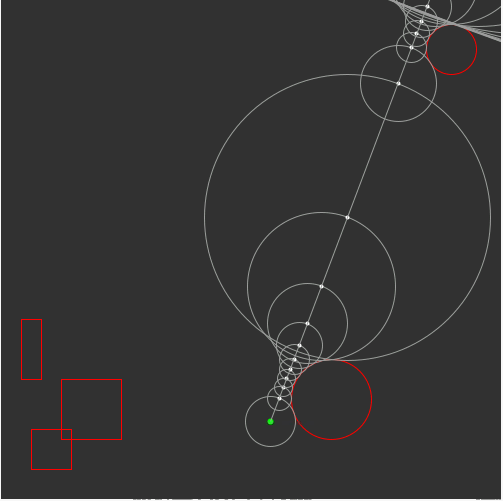
\includegraphics[width=8cm]{images/marching.png}
\begin{figure}[h]
    \centering
    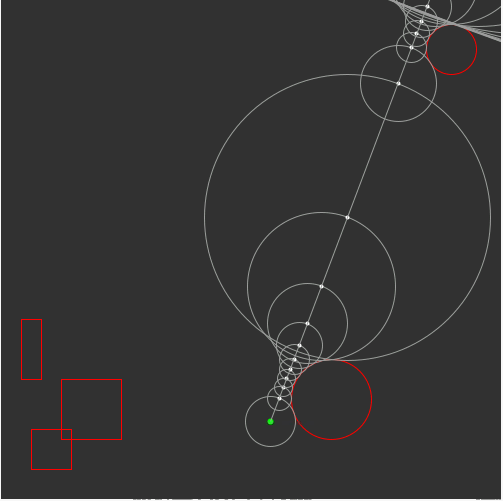
\includegraphics[width=8cm]{images/marching.png}
    \caption{Illustration 2D de la marche point par point d'un rayon (plus de details dans \ref{subsec:projection} \nameref{subsec:projection})}
    \label{fig:my_label}
\end{figure}

\clearpage
\documentclass[a4paper,11pt,twoside]{article} 
%\documentclass{article}


\author{Victor LASSERRE \& Valentin SERVIERES}
\pdfminorversion=7 % To use charte graphique (pdf 1.7)
\usepackage[utf8]{inputenc}
\usepackage[T1]{fontenc}
\usepackage{lscape}
\usepackage{boldline,multirow,tabularx,colortbl,makecell,fancybox,amsfonts,amssymb,amsmath,mathrsfs,array, svg}
\usepackage{pgf,tikz,xcolor,graphicx}
\usetikzlibrary{calc,positioning,shapes.geometric,shapes.symbols,shapes.misc, fit, shapes, arrows, arrows.meta,fadings,through}
\usepackage[top=2cm, bottom=2cm, left=2cm, right=2cm]{geometry}
\usepackage{hyperref,titlesec,eurosym,eso-pic,float}
\usepackage[french]{babel}
%\usepackage{bibleref} ajouté par moi mais flemme
% minted et les encars de code en gros
%\usepackage[newfloat]{minted}
\usepackage{caption}
\usepackage{tcolorbox}
%\newenvironment{code}{\captionsetup{type=listing}}{}
%\SetupFloatingEnvironment{listing}{name=Code Source}

% table des annexes
\usepackage{minitoc}
\usepackage{pdfpages}

% bibliographie
%\usepackage{biblatex}
%\usepackage{csquotes}
%\addbibresource{bibliography.bib}

%\input{advanced.params/listings.conf}
\input{charteINSA/advanced.params/tikz.conf}
\input{charteINSA/advanced.params/misc.commands}
\input{charteINSA/cover/covermain.tex}



%\usepackage[french]{babel}

% resolve no citation problem
\nocite{*}
%\usepackage[...,backend=bibtex]{biblatex}

% Set page size and margins
% Replace `letterpaper' with `a4paper' for UK/EU standard size
%%%%%\usepackage[letterpaper,top=2cm,bottom=2cm,left=3cm,right=3cm,marginparwidth=1.75cm]{geometry}

% Useful packages
\usepackage{listings}

\input{preferences/listings-glsl.prf}
% optionally set GLSL as default language
\lstset{language=GLSL}
\lstset{
  breaklines=true,
  breakatwhitespace=true,
  numbers=left,
  basicstyle={\small\ttfamily},
  numberstyle=\tiny\color{gray},
  tabsize=3,% end normal settings
  breaklines=true,                              % break long lines
  commentstyle=\itshape\color{green},           % comments are green
  keywordstyle=[1]\color{blue},                 % instructions are blue
  keywordstyle=[2]\color{orange},               % sections/other directives are orange
  keywordstyle=[3]\color{red},                   % registers are red
  stringstyle=\color{mauve},                    % strings are from the telekom
  identifierstyle=\color{teal},                 % user declared addresses are teal
  frame=l,                                      % black line on the left side of code
  language=GLSL,                   % all code is RISC-V
  tabsize=4,                                    % indent tabs with 4 spaces
  showstringspaces=false                        % do not replace spaces with weird underlines
}

\usepackage[square,numbers]{natbib}
\bibliographystyle{abbrvnat}
%Includes "References" in the table of contents
\usepackage[nottoc]{tocbibind}

\usepackage{setspace}
\usepackage{titletoc}
%\usepackage[T1]{fontenc}
%\usepackage{amsfonts}
%\usepackage{graphicx}
\usepackage{mathtools}
\graphicspath{ {images/} }

%\usepackage{fancyhdr}
\pagestyle{fancy}
\renewcommand\headrulewidth{1pt}
\fancyhead[L]{\textsf{Moteur graphique}}
\fancyhead[R]{\textsf{}}
%\usepackage[colorlinks=true, allcolors=blue]{hyperref}


\begin{document}
\dosecttoc{} % generate TOC
%\maketitle
\clearpage

% Remerciements
\thispagestyle{empty} % removes page number
\subsection*{Remerciements}
Nous tenons à remercier notre tuteur de projet M. Sanchez, notamment pour son aide précieuse et ses conseils. \\
Nous remercions également Inigo Quilez pour la riche documentation sur le ray marching qu'il fournit librement sur son site web.
\clearpage

% TABLE DES MATIÈRES
\thispagestyle{empty} % removes page number
\setcounter{secnumdepth}{3}
\tableofcontents
\clearpage

\setcounter{page}{1}


\sectionnn{Introduction}

    Engin Pas Tangible est un moteur graphique reposant sur le principe de Ray Marching : un système de 3D similaire au Ray Tracing, mais beaucoup plus rarement utilisé. Ce système a certains avantages par rapport au Ray Tracing, comme par exemple de permettre une implémetation peu coûteuse de fractales, ou autres figures se reproduisant à l'identique. \\
    Le Ray Marching repose sur la projection de rayons depuis une camera vers la scene. Pour projeter un rayon, on le fait avancer pas à pas (\emph{Marching}). La distance des pas doit être la plus grande possible, mais sans que le rayon ne traverse d'objet de la scene 3D.
\\
\\
%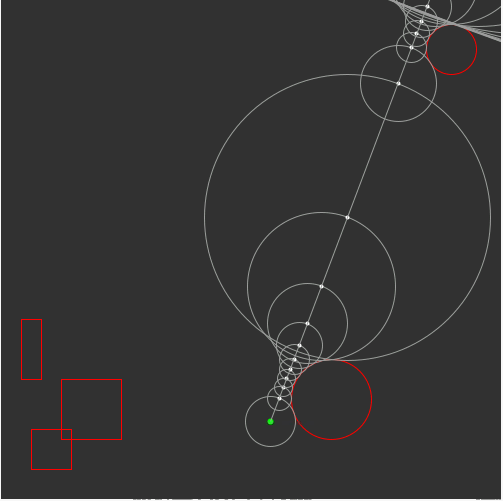
\includegraphics[width=8cm]{images/marching.png}
\begin{figure}[h]
    \centering
    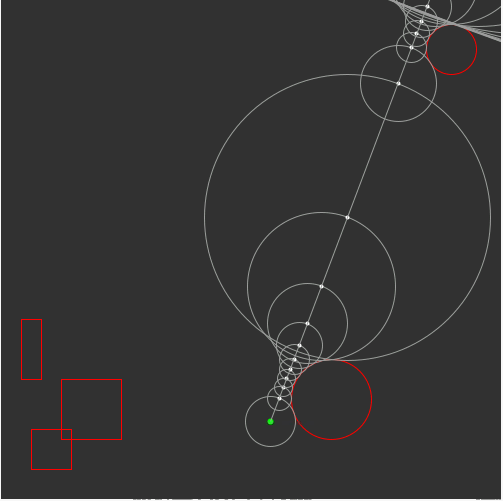
\includegraphics[width=8cm]{images/marching.png}
    \caption{Illustration 2D de la marche point par point d'un rayon (plus de details dans \ref{subsec:projection} \nameref{subsec:projection})}
    \label{fig:my_label}
\end{figure}

\clearpage
\documentclass[a4paper,11pt,twoside]{article} 
%\documentclass{article}

\input{charteINSA/maincharte.tex}

%\usepackage[french]{babel}

% resolve no citation problem
\nocite{*}
%\usepackage[...,backend=bibtex]{biblatex}

% Set page size and margins
% Replace `letterpaper' with `a4paper' for UK/EU standard size
%%%%%\usepackage[letterpaper,top=2cm,bottom=2cm,left=3cm,right=3cm,marginparwidth=1.75cm]{geometry}

% Useful packages
\usepackage{listings}

\input{preferences/listings-glsl.prf}
% optionally set GLSL as default language
\lstset{language=GLSL}
\input{preferences/glsl.tex}

\usepackage[square,numbers]{natbib}
\bibliographystyle{abbrvnat}
%Includes "References" in the table of contents
\usepackage[nottoc]{tocbibind}

\usepackage{setspace}
\usepackage{titletoc}
%\usepackage[T1]{fontenc}
%\usepackage{amsfonts}
%\usepackage{graphicx}
\usepackage{mathtools}
\graphicspath{ {images/} }

%\input{hautdepage.tex}
%\usepackage[colorlinks=true, allcolors=blue]{hyperref}


\begin{document}
\dosecttoc{} % generate TOC
%\maketitle
\clearpage

% Remerciements
\thispagestyle{empty} % removes page number
\subsection*{Remerciements}
Nous tenons à remercier notre tuteur de projet M. Sanchez, notamment pour son aide précieuse et ses conseils. \\
Nous remercions également Inigo Quilez pour la riche documentation sur le ray marching qu'il fournit librement sur son site web.
\clearpage

% TABLE DES MATIÈRES
\thispagestyle{empty} % removes page number
\setcounter{secnumdepth}{3}
\tableofcontents
\clearpage

\setcounter{page}{1}


\input{Parties/Introduction}
\clearpage
\input{Parties/Fonctionnement/main}
\clearpage
\input{Parties/Fonctionnalites/main}
\clearpage
\input{Parties/Historique/main}
\clearpage
\input{Parties/Conclusion}

\clearpage


%Imports the bibliography file "sample.bib"
\bibliography{sample}
\clearpage

% TABLE DES ANNEXES
\clearpage
\appendix
%\thispagestyle{empty} % removes page number
\sectionnn{Table des Annexes}
\addtocontents{toc}{\protect\setcounter{tocdepth}{0}}
\renewcommand{\stctitle}{}                          % Titre (issue with previous subsection showing up)
\renewcommand\thesubsection{A\arabic{subsection}}   % Numérotation
\renewcommand{\stcSSfont}{}                         % Police normale, pas en gras
\mtcsetrules{secttoc}{off}                          % Désactivation des lignes en haut et en bas de la table

% Affichage de la table des annexes
\secttoc
% ANNEXES
\clearpage
\pagenumbering{Roman}


\input{Parties/Annexes}

\mtcsetrules{secttoc}{off}

\end{document}


                        

\clearpage
\documentclass[a4paper,11pt,twoside]{article} 
%\documentclass{article}

\input{charteINSA/maincharte.tex}

%\usepackage[french]{babel}

% resolve no citation problem
\nocite{*}
%\usepackage[...,backend=bibtex]{biblatex}

% Set page size and margins
% Replace `letterpaper' with `a4paper' for UK/EU standard size
%%%%%\usepackage[letterpaper,top=2cm,bottom=2cm,left=3cm,right=3cm,marginparwidth=1.75cm]{geometry}

% Useful packages
\usepackage{listings}

\input{preferences/listings-glsl.prf}
% optionally set GLSL as default language
\lstset{language=GLSL}
\input{preferences/glsl.tex}

\usepackage[square,numbers]{natbib}
\bibliographystyle{abbrvnat}
%Includes "References" in the table of contents
\usepackage[nottoc]{tocbibind}

\usepackage{setspace}
\usepackage{titletoc}
%\usepackage[T1]{fontenc}
%\usepackage{amsfonts}
%\usepackage{graphicx}
\usepackage{mathtools}
\graphicspath{ {images/} }

%\input{hautdepage.tex}
%\usepackage[colorlinks=true, allcolors=blue]{hyperref}


\begin{document}
\dosecttoc{} % generate TOC
%\maketitle
\clearpage

% Remerciements
\thispagestyle{empty} % removes page number
\subsection*{Remerciements}
Nous tenons à remercier notre tuteur de projet M. Sanchez, notamment pour son aide précieuse et ses conseils. \\
Nous remercions également Inigo Quilez pour la riche documentation sur le ray marching qu'il fournit librement sur son site web.
\clearpage

% TABLE DES MATIÈRES
\thispagestyle{empty} % removes page number
\setcounter{secnumdepth}{3}
\tableofcontents
\clearpage

\setcounter{page}{1}


\input{Parties/Introduction}
\clearpage
\input{Parties/Fonctionnement/main}
\clearpage
\input{Parties/Fonctionnalites/main}
\clearpage
\input{Parties/Historique/main}
\clearpage
\input{Parties/Conclusion}

\clearpage


%Imports the bibliography file "sample.bib"
\bibliography{sample}
\clearpage

% TABLE DES ANNEXES
\clearpage
\appendix
%\thispagestyle{empty} % removes page number
\sectionnn{Table des Annexes}
\addtocontents{toc}{\protect\setcounter{tocdepth}{0}}
\renewcommand{\stctitle}{}                          % Titre (issue with previous subsection showing up)
\renewcommand\thesubsection{A\arabic{subsection}}   % Numérotation
\renewcommand{\stcSSfont}{}                         % Police normale, pas en gras
\mtcsetrules{secttoc}{off}                          % Désactivation des lignes en haut et en bas de la table

% Affichage de la table des annexes
\secttoc
% ANNEXES
\clearpage
\pagenumbering{Roman}


\input{Parties/Annexes}

\mtcsetrules{secttoc}{off}

\end{document}


                        

\clearpage
\documentclass[a4paper,11pt,twoside]{article} 
%\documentclass{article}

\input{charteINSA/maincharte.tex}

%\usepackage[french]{babel}

% resolve no citation problem
\nocite{*}
%\usepackage[...,backend=bibtex]{biblatex}

% Set page size and margins
% Replace `letterpaper' with `a4paper' for UK/EU standard size
%%%%%\usepackage[letterpaper,top=2cm,bottom=2cm,left=3cm,right=3cm,marginparwidth=1.75cm]{geometry}

% Useful packages
\usepackage{listings}

\input{preferences/listings-glsl.prf}
% optionally set GLSL as default language
\lstset{language=GLSL}
\input{preferences/glsl.tex}

\usepackage[square,numbers]{natbib}
\bibliographystyle{abbrvnat}
%Includes "References" in the table of contents
\usepackage[nottoc]{tocbibind}

\usepackage{setspace}
\usepackage{titletoc}
%\usepackage[T1]{fontenc}
%\usepackage{amsfonts}
%\usepackage{graphicx}
\usepackage{mathtools}
\graphicspath{ {images/} }

%\input{hautdepage.tex}
%\usepackage[colorlinks=true, allcolors=blue]{hyperref}


\begin{document}
\dosecttoc{} % generate TOC
%\maketitle
\clearpage

% Remerciements
\thispagestyle{empty} % removes page number
\subsection*{Remerciements}
Nous tenons à remercier notre tuteur de projet M. Sanchez, notamment pour son aide précieuse et ses conseils. \\
Nous remercions également Inigo Quilez pour la riche documentation sur le ray marching qu'il fournit librement sur son site web.
\clearpage

% TABLE DES MATIÈRES
\thispagestyle{empty} % removes page number
\setcounter{secnumdepth}{3}
\tableofcontents
\clearpage

\setcounter{page}{1}


\input{Parties/Introduction}
\clearpage
\input{Parties/Fonctionnement/main}
\clearpage
\input{Parties/Fonctionnalites/main}
\clearpage
\input{Parties/Historique/main}
\clearpage
\input{Parties/Conclusion}

\clearpage


%Imports the bibliography file "sample.bib"
\bibliography{sample}
\clearpage

% TABLE DES ANNEXES
\clearpage
\appendix
%\thispagestyle{empty} % removes page number
\sectionnn{Table des Annexes}
\addtocontents{toc}{\protect\setcounter{tocdepth}{0}}
\renewcommand{\stctitle}{}                          % Titre (issue with previous subsection showing up)
\renewcommand\thesubsection{A\arabic{subsection}}   % Numérotation
\renewcommand{\stcSSfont}{}                         % Police normale, pas en gras
\mtcsetrules{secttoc}{off}                          % Désactivation des lignes en haut et en bas de la table

% Affichage de la table des annexes
\secttoc
% ANNEXES
\clearpage
\pagenumbering{Roman}


\input{Parties/Annexes}

\mtcsetrules{secttoc}{off}

\end{document}


                        

\clearpage
\sectionnn{Conclusion}

Ce projet a été captivant et très motivant. Le fait de pouvoir observer rapidement les résultats de notre code était très agréable.\\
Nous avons rempli et même dépassé les objectifs que nous nous étions fixés.\\
Il était également intéressant de retrouver des notions vues en maths à l'INSA dans une application concrète.\\ \par

L'expérience fut très enrichissante car nous avons dû nous organiser pour pouvoir travailler en binôme sur le même code avec l'utilisation d'un gestionnaire de version (git) auquel nous nous sommes formés.\\
Nous avons pu explorer le principe du Ray Marching, découvrir un nouveau langage, le GLSL, ainsi que les bases de développement logiciel.\\ \par

Ce rapport était également l'occasion d'apprendre à maîtriser le LaTeX, mais c'était surtout l'occasion d'expliquer de façon claire et concise un concept technique.\\ \par

Finalement, ce projet de moteur graphique nous a beaucoup apporté et nous pensons continuer à le développer dans le futur.

\clearpage


%Imports the bibliography file "sample.bib"
\bibliography{sample}
\clearpage

% TABLE DES ANNEXES
\clearpage
\appendix
%\thispagestyle{empty} % removes page number
\sectionnn{Table des Annexes}
\addtocontents{toc}{\protect\setcounter{tocdepth}{0}}
\renewcommand{\stctitle}{}                          % Titre (issue with previous subsection showing up)
\renewcommand\thesubsection{A\arabic{subsection}}   % Numérotation
\renewcommand{\stcSSfont}{}                         % Police normale, pas en gras
\mtcsetrules{secttoc}{off}                          % Désactivation des lignes en haut et en bas de la table

% Affichage de la table des annexes
\secttoc
% ANNEXES
\clearpage
\pagenumbering{Roman}


\subsection{Scène simple}
%\addcontentsline{toc}{section}{Scène simple}
Code à mettre dans un fichier, nommé \emph{example.fs} par exemple
\begin{lstlisting}[language=GLSL]
#version 330 core
in vec2 FragCoord;
in float Time;
in vec2 MousePos;
in vec3 CamPos;
in vec3 CamDir;

out vec4 FragColor;
//uniform sampler2D generalTexture;

float SDF_Box_Frame( vec3 p, vec3 b, float e )
{
       p = abs(p  )-b;
  vec3 q = abs(p+e)-e;
  return min(min(
      length(max(vec3(p.x,q.y,q.z),0.0))+min(max(p.x,max(q.y,q.z)),0.0),
      length(max(vec3(q.x,p.y,q.z),0.0))+min(max(q.x,max(p.y,q.z)),0.0)),
      length(max(vec3(q.x,q.y,p.z),0.0))+min(max(q.x,max(q.y,p.z)),0.0));
}

float SDF_Circle(vec3 p,float r){
    return length(p)-r;
}

float SDF_Global(vec3 p){
    return min(
        SDF_Box_Frame(p,vec3(.5,.5,.5),0.1),
        SDF_Circle(mod(p+vec3(.5),vec3(1.,1.,1.))-vec3(.5),.15));
}

vec4 Get_Impact(vec3 origin,vec3 dir){//must have length(dir)==1 
    vec3 pos=origin;
    float dist;
    for(int i=0;i<30;i++){
        dist=SDF_Global(pos);
        pos+=dist*dir;
        if(dist<=.01) return vec4(pos,1.);
        if(dist>=20.0) return vec4(pos,-1.);
    }
    return vec4(pos,-1.);
}

vec3 grad(vec3 p){
    vec2 epsilon = vec2(.01,0.);
    return normalize(vec3(SDF_Global(p+epsilon.xyy)-SDF_Global(p-epsilon.xyy),
    SDF_Global(p+epsilon.yxy)-SDF_Global(p-epsilon.yxy),
    SDF_Global(p+epsilon.yyx)-SDF_Global(p-epsilon.yyx)));
}

vec3 Get_Color(vec3 origin,vec3 dir){
    vec4 impact = Get_Impact(origin,dir);
    if(impact.w<0.) return vec3(.5,.7,1.);
    vec3 normale=grad(impact.xyz);
    return normale;
}

void main()
{
    vec3 lookingAt = vec3(0.,0.,0.);
    vec3 posCam    = vec3(3.*sin(Time*.5),0.,3.*cos(Time*.5));
    
    vec3 ez = normalize(lookingAt - posCam); //base orthonormee
    vec3 ex = normalize(cross(ez,vec3(0.,1.,0.)));
    vec3 ey = cross(ex,ez);
    
    vec3 dir = normalize(FragCoord.x * ex + FragCoord.y*ey + 1.*ez);
    
  FragColor=vec4(Get_Color(posCam,dir),1.);
}
\end{lstlisting}

\mtcsetrules{secttoc}{off}

\end{document}


                        

\clearpage
\documentclass[a4paper,11pt,twoside]{article} 
%\documentclass{article}


\author{Victor LASSERRE \& Valentin SERVIERES}
\pdfminorversion=7 % To use charte graphique (pdf 1.7)
\usepackage[utf8]{inputenc}
\usepackage[T1]{fontenc}
\usepackage{lscape}
\usepackage{boldline,multirow,tabularx,colortbl,makecell,fancybox,amsfonts,amssymb,amsmath,mathrsfs,array, svg}
\usepackage{pgf,tikz,xcolor,graphicx}
\usetikzlibrary{calc,positioning,shapes.geometric,shapes.symbols,shapes.misc, fit, shapes, arrows, arrows.meta,fadings,through}
\usepackage[top=2cm, bottom=2cm, left=2cm, right=2cm]{geometry}
\usepackage{hyperref,titlesec,eurosym,eso-pic,float}
\usepackage[french]{babel}
%\usepackage{bibleref} ajouté par moi mais flemme
% minted et les encars de code en gros
%\usepackage[newfloat]{minted}
\usepackage{caption}
\usepackage{tcolorbox}
%\newenvironment{code}{\captionsetup{type=listing}}{}
%\SetupFloatingEnvironment{listing}{name=Code Source}

% table des annexes
\usepackage{minitoc}
\usepackage{pdfpages}

% bibliographie
%\usepackage{biblatex}
%\usepackage{csquotes}
%\addbibresource{bibliography.bib}

%\input{advanced.params/listings.conf}
\input{charteINSA/advanced.params/tikz.conf}
\input{charteINSA/advanced.params/misc.commands}
\input{charteINSA/cover/covermain.tex}



%\usepackage[french]{babel}

% resolve no citation problem
\nocite{*}
%\usepackage[...,backend=bibtex]{biblatex}

% Set page size and margins
% Replace `letterpaper' with `a4paper' for UK/EU standard size
%%%%%\usepackage[letterpaper,top=2cm,bottom=2cm,left=3cm,right=3cm,marginparwidth=1.75cm]{geometry}

% Useful packages
\usepackage{listings}

\input{preferences/listings-glsl.prf}
% optionally set GLSL as default language
\lstset{language=GLSL}
\lstset{
  breaklines=true,
  breakatwhitespace=true,
  numbers=left,
  basicstyle={\small\ttfamily},
  numberstyle=\tiny\color{gray},
  tabsize=3,% end normal settings
  breaklines=true,                              % break long lines
  commentstyle=\itshape\color{green},           % comments are green
  keywordstyle=[1]\color{blue},                 % instructions are blue
  keywordstyle=[2]\color{orange},               % sections/other directives are orange
  keywordstyle=[3]\color{red},                   % registers are red
  stringstyle=\color{mauve},                    % strings are from the telekom
  identifierstyle=\color{teal},                 % user declared addresses are teal
  frame=l,                                      % black line on the left side of code
  language=GLSL,                   % all code is RISC-V
  tabsize=4,                                    % indent tabs with 4 spaces
  showstringspaces=false                        % do not replace spaces with weird underlines
}

\usepackage[square,numbers]{natbib}
\bibliographystyle{abbrvnat}
%Includes "References" in the table of contents
\usepackage[nottoc]{tocbibind}

\usepackage{setspace}
\usepackage{titletoc}
%\usepackage[T1]{fontenc}
%\usepackage{amsfonts}
%\usepackage{graphicx}
\usepackage{mathtools}
\graphicspath{ {images/} }

%\usepackage{fancyhdr}
\pagestyle{fancy}
\renewcommand\headrulewidth{1pt}
\fancyhead[L]{\textsf{Moteur graphique}}
\fancyhead[R]{\textsf{}}
%\usepackage[colorlinks=true, allcolors=blue]{hyperref}


\begin{document}
\dosecttoc{} % generate TOC
%\maketitle
\clearpage

% Remerciements
\thispagestyle{empty} % removes page number
\subsection*{Remerciements}
Nous tenons à remercier notre tuteur de projet M. Sanchez, notamment pour son aide précieuse et ses conseils. \\
Nous remercions également Inigo Quilez pour la riche documentation sur le ray marching qu'il fournit librement sur son site web.
\clearpage

% TABLE DES MATIÈRES
\thispagestyle{empty} % removes page number
\setcounter{secnumdepth}{3}
\tableofcontents
\clearpage

\setcounter{page}{1}


\sectionnn{Introduction}

    Engin Pas Tangible est un moteur graphique reposant sur le principe de Ray Marching : un système de 3D similaire au Ray Tracing, mais beaucoup plus rarement utilisé. Ce système a certains avantages par rapport au Ray Tracing, comme par exemple de permettre une implémetation peu coûteuse de fractales, ou autres figures se reproduisant à l'identique. \\
    Le Ray Marching repose sur la projection de rayons depuis une camera vers la scene. Pour projeter un rayon, on le fait avancer pas à pas (\emph{Marching}). La distance des pas doit être la plus grande possible, mais sans que le rayon ne traverse d'objet de la scene 3D.
\\
\\
%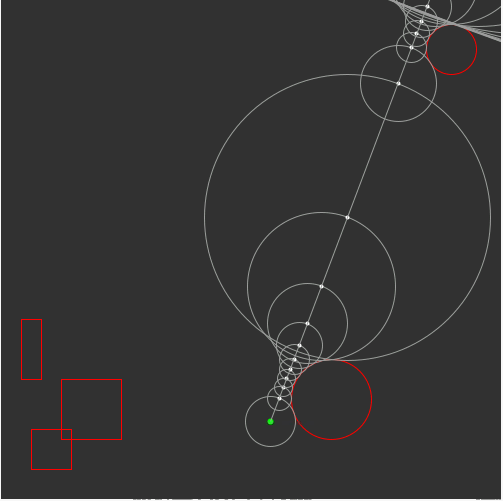
\includegraphics[width=8cm]{images/marching.png}
\begin{figure}[h]
    \centering
    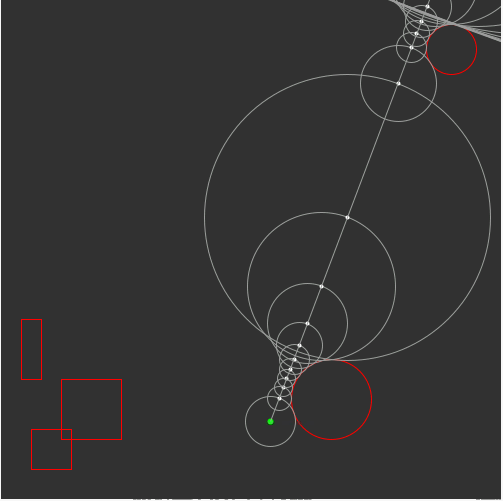
\includegraphics[width=8cm]{images/marching.png}
    \caption{Illustration 2D de la marche point par point d'un rayon (plus de details dans \ref{subsec:projection} \nameref{subsec:projection})}
    \label{fig:my_label}
\end{figure}

\clearpage
\documentclass[a4paper,11pt,twoside]{article} 
%\documentclass{article}

\input{charteINSA/maincharte.tex}

%\usepackage[french]{babel}

% resolve no citation problem
\nocite{*}
%\usepackage[...,backend=bibtex]{biblatex}

% Set page size and margins
% Replace `letterpaper' with `a4paper' for UK/EU standard size
%%%%%\usepackage[letterpaper,top=2cm,bottom=2cm,left=3cm,right=3cm,marginparwidth=1.75cm]{geometry}

% Useful packages
\usepackage{listings}

\input{preferences/listings-glsl.prf}
% optionally set GLSL as default language
\lstset{language=GLSL}
\input{preferences/glsl.tex}

\usepackage[square,numbers]{natbib}
\bibliographystyle{abbrvnat}
%Includes "References" in the table of contents
\usepackage[nottoc]{tocbibind}

\usepackage{setspace}
\usepackage{titletoc}
%\usepackage[T1]{fontenc}
%\usepackage{amsfonts}
%\usepackage{graphicx}
\usepackage{mathtools}
\graphicspath{ {images/} }

%\input{hautdepage.tex}
%\usepackage[colorlinks=true, allcolors=blue]{hyperref}


\begin{document}
\dosecttoc{} % generate TOC
%\maketitle
\clearpage

% Remerciements
\thispagestyle{empty} % removes page number
\subsection*{Remerciements}
Nous tenons à remercier notre tuteur de projet M. Sanchez, notamment pour son aide précieuse et ses conseils. \\
Nous remercions également Inigo Quilez pour la riche documentation sur le ray marching qu'il fournit librement sur son site web.
\clearpage

% TABLE DES MATIÈRES
\thispagestyle{empty} % removes page number
\setcounter{secnumdepth}{3}
\tableofcontents
\clearpage

\setcounter{page}{1}


\input{Parties/Introduction}
\clearpage
\input{Parties/Fonctionnement/main}
\clearpage
\input{Parties/Fonctionnalites/main}
\clearpage
\input{Parties/Historique/main}
\clearpage
\input{Parties/Conclusion}

\clearpage


%Imports the bibliography file "sample.bib"
\bibliography{sample}
\clearpage

% TABLE DES ANNEXES
\clearpage
\appendix
%\thispagestyle{empty} % removes page number
\sectionnn{Table des Annexes}
\addtocontents{toc}{\protect\setcounter{tocdepth}{0}}
\renewcommand{\stctitle}{}                          % Titre (issue with previous subsection showing up)
\renewcommand\thesubsection{A\arabic{subsection}}   % Numérotation
\renewcommand{\stcSSfont}{}                         % Police normale, pas en gras
\mtcsetrules{secttoc}{off}                          % Désactivation des lignes en haut et en bas de la table

% Affichage de la table des annexes
\secttoc
% ANNEXES
\clearpage
\pagenumbering{Roman}


\input{Parties/Annexes}

\mtcsetrules{secttoc}{off}

\end{document}


                        

\clearpage
\documentclass[a4paper,11pt,twoside]{article} 
%\documentclass{article}

\input{charteINSA/maincharte.tex}

%\usepackage[french]{babel}

% resolve no citation problem
\nocite{*}
%\usepackage[...,backend=bibtex]{biblatex}

% Set page size and margins
% Replace `letterpaper' with `a4paper' for UK/EU standard size
%%%%%\usepackage[letterpaper,top=2cm,bottom=2cm,left=3cm,right=3cm,marginparwidth=1.75cm]{geometry}

% Useful packages
\usepackage{listings}

\input{preferences/listings-glsl.prf}
% optionally set GLSL as default language
\lstset{language=GLSL}
\input{preferences/glsl.tex}

\usepackage[square,numbers]{natbib}
\bibliographystyle{abbrvnat}
%Includes "References" in the table of contents
\usepackage[nottoc]{tocbibind}

\usepackage{setspace}
\usepackage{titletoc}
%\usepackage[T1]{fontenc}
%\usepackage{amsfonts}
%\usepackage{graphicx}
\usepackage{mathtools}
\graphicspath{ {images/} }

%\input{hautdepage.tex}
%\usepackage[colorlinks=true, allcolors=blue]{hyperref}


\begin{document}
\dosecttoc{} % generate TOC
%\maketitle
\clearpage

% Remerciements
\thispagestyle{empty} % removes page number
\subsection*{Remerciements}
Nous tenons à remercier notre tuteur de projet M. Sanchez, notamment pour son aide précieuse et ses conseils. \\
Nous remercions également Inigo Quilez pour la riche documentation sur le ray marching qu'il fournit librement sur son site web.
\clearpage

% TABLE DES MATIÈRES
\thispagestyle{empty} % removes page number
\setcounter{secnumdepth}{3}
\tableofcontents
\clearpage

\setcounter{page}{1}


\input{Parties/Introduction}
\clearpage
\input{Parties/Fonctionnement/main}
\clearpage
\input{Parties/Fonctionnalites/main}
\clearpage
\input{Parties/Historique/main}
\clearpage
\input{Parties/Conclusion}

\clearpage


%Imports the bibliography file "sample.bib"
\bibliography{sample}
\clearpage

% TABLE DES ANNEXES
\clearpage
\appendix
%\thispagestyle{empty} % removes page number
\sectionnn{Table des Annexes}
\addtocontents{toc}{\protect\setcounter{tocdepth}{0}}
\renewcommand{\stctitle}{}                          % Titre (issue with previous subsection showing up)
\renewcommand\thesubsection{A\arabic{subsection}}   % Numérotation
\renewcommand{\stcSSfont}{}                         % Police normale, pas en gras
\mtcsetrules{secttoc}{off}                          % Désactivation des lignes en haut et en bas de la table

% Affichage de la table des annexes
\secttoc
% ANNEXES
\clearpage
\pagenumbering{Roman}


\input{Parties/Annexes}

\mtcsetrules{secttoc}{off}

\end{document}


                        

\clearpage
\documentclass[a4paper,11pt,twoside]{article} 
%\documentclass{article}

\input{charteINSA/maincharte.tex}

%\usepackage[french]{babel}

% resolve no citation problem
\nocite{*}
%\usepackage[...,backend=bibtex]{biblatex}

% Set page size and margins
% Replace `letterpaper' with `a4paper' for UK/EU standard size
%%%%%\usepackage[letterpaper,top=2cm,bottom=2cm,left=3cm,right=3cm,marginparwidth=1.75cm]{geometry}

% Useful packages
\usepackage{listings}

\input{preferences/listings-glsl.prf}
% optionally set GLSL as default language
\lstset{language=GLSL}
\input{preferences/glsl.tex}

\usepackage[square,numbers]{natbib}
\bibliographystyle{abbrvnat}
%Includes "References" in the table of contents
\usepackage[nottoc]{tocbibind}

\usepackage{setspace}
\usepackage{titletoc}
%\usepackage[T1]{fontenc}
%\usepackage{amsfonts}
%\usepackage{graphicx}
\usepackage{mathtools}
\graphicspath{ {images/} }

%\input{hautdepage.tex}
%\usepackage[colorlinks=true, allcolors=blue]{hyperref}


\begin{document}
\dosecttoc{} % generate TOC
%\maketitle
\clearpage

% Remerciements
\thispagestyle{empty} % removes page number
\subsection*{Remerciements}
Nous tenons à remercier notre tuteur de projet M. Sanchez, notamment pour son aide précieuse et ses conseils. \\
Nous remercions également Inigo Quilez pour la riche documentation sur le ray marching qu'il fournit librement sur son site web.
\clearpage

% TABLE DES MATIÈRES
\thispagestyle{empty} % removes page number
\setcounter{secnumdepth}{3}
\tableofcontents
\clearpage

\setcounter{page}{1}


\input{Parties/Introduction}
\clearpage
\input{Parties/Fonctionnement/main}
\clearpage
\input{Parties/Fonctionnalites/main}
\clearpage
\input{Parties/Historique/main}
\clearpage
\input{Parties/Conclusion}

\clearpage


%Imports the bibliography file "sample.bib"
\bibliography{sample}
\clearpage

% TABLE DES ANNEXES
\clearpage
\appendix
%\thispagestyle{empty} % removes page number
\sectionnn{Table des Annexes}
\addtocontents{toc}{\protect\setcounter{tocdepth}{0}}
\renewcommand{\stctitle}{}                          % Titre (issue with previous subsection showing up)
\renewcommand\thesubsection{A\arabic{subsection}}   % Numérotation
\renewcommand{\stcSSfont}{}                         % Police normale, pas en gras
\mtcsetrules{secttoc}{off}                          % Désactivation des lignes en haut et en bas de la table

% Affichage de la table des annexes
\secttoc
% ANNEXES
\clearpage
\pagenumbering{Roman}


\input{Parties/Annexes}

\mtcsetrules{secttoc}{off}

\end{document}


                        

\clearpage
\sectionnn{Conclusion}

Ce projet a été captivant et très motivant. Le fait de pouvoir observer rapidement les résultats de notre code était très agréable.\\
Nous avons rempli et même dépassé les objectifs que nous nous étions fixés.\\
Il était également intéressant de retrouver des notions vues en maths à l'INSA dans une application concrète.\\ \par

L'expérience fut très enrichissante car nous avons dû nous organiser pour pouvoir travailler en binôme sur le même code avec l'utilisation d'un gestionnaire de version (git) auquel nous nous sommes formés.\\
Nous avons pu explorer le principe du Ray Marching, découvrir un nouveau langage, le GLSL, ainsi que les bases de développement logiciel.\\ \par

Ce rapport était également l'occasion d'apprendre à maîtriser le LaTeX, mais c'était surtout l'occasion d'expliquer de façon claire et concise un concept technique.\\ \par

Finalement, ce projet de moteur graphique nous a beaucoup apporté et nous pensons continuer à le développer dans le futur.

\clearpage


%Imports the bibliography file "sample.bib"
\bibliography{sample}
\clearpage

% TABLE DES ANNEXES
\clearpage
\appendix
%\thispagestyle{empty} % removes page number
\sectionnn{Table des Annexes}
\addtocontents{toc}{\protect\setcounter{tocdepth}{0}}
\renewcommand{\stctitle}{}                          % Titre (issue with previous subsection showing up)
\renewcommand\thesubsection{A\arabic{subsection}}   % Numérotation
\renewcommand{\stcSSfont}{}                         % Police normale, pas en gras
\mtcsetrules{secttoc}{off}                          % Désactivation des lignes en haut et en bas de la table

% Affichage de la table des annexes
\secttoc
% ANNEXES
\clearpage
\pagenumbering{Roman}


\subsection{Scène simple}
%\addcontentsline{toc}{section}{Scène simple}
Code à mettre dans un fichier, nommé \emph{example.fs} par exemple
\begin{lstlisting}[language=GLSL]
#version 330 core
in vec2 FragCoord;
in float Time;
in vec2 MousePos;
in vec3 CamPos;
in vec3 CamDir;

out vec4 FragColor;
//uniform sampler2D generalTexture;

float SDF_Box_Frame( vec3 p, vec3 b, float e )
{
       p = abs(p  )-b;
  vec3 q = abs(p+e)-e;
  return min(min(
      length(max(vec3(p.x,q.y,q.z),0.0))+min(max(p.x,max(q.y,q.z)),0.0),
      length(max(vec3(q.x,p.y,q.z),0.0))+min(max(q.x,max(p.y,q.z)),0.0)),
      length(max(vec3(q.x,q.y,p.z),0.0))+min(max(q.x,max(q.y,p.z)),0.0));
}

float SDF_Circle(vec3 p,float r){
    return length(p)-r;
}

float SDF_Global(vec3 p){
    return min(
        SDF_Box_Frame(p,vec3(.5,.5,.5),0.1),
        SDF_Circle(mod(p+vec3(.5),vec3(1.,1.,1.))-vec3(.5),.15));
}

vec4 Get_Impact(vec3 origin,vec3 dir){//must have length(dir)==1 
    vec3 pos=origin;
    float dist;
    for(int i=0;i<30;i++){
        dist=SDF_Global(pos);
        pos+=dist*dir;
        if(dist<=.01) return vec4(pos,1.);
        if(dist>=20.0) return vec4(pos,-1.);
    }
    return vec4(pos,-1.);
}

vec3 grad(vec3 p){
    vec2 epsilon = vec2(.01,0.);
    return normalize(vec3(SDF_Global(p+epsilon.xyy)-SDF_Global(p-epsilon.xyy),
    SDF_Global(p+epsilon.yxy)-SDF_Global(p-epsilon.yxy),
    SDF_Global(p+epsilon.yyx)-SDF_Global(p-epsilon.yyx)));
}

vec3 Get_Color(vec3 origin,vec3 dir){
    vec4 impact = Get_Impact(origin,dir);
    if(impact.w<0.) return vec3(.5,.7,1.);
    vec3 normale=grad(impact.xyz);
    return normale;
}

void main()
{
    vec3 lookingAt = vec3(0.,0.,0.);
    vec3 posCam    = vec3(3.*sin(Time*.5),0.,3.*cos(Time*.5));
    
    vec3 ez = normalize(lookingAt - posCam); //base orthonormee
    vec3 ex = normalize(cross(ez,vec3(0.,1.,0.)));
    vec3 ey = cross(ex,ez);
    
    vec3 dir = normalize(FragCoord.x * ex + FragCoord.y*ey + 1.*ez);
    
  FragColor=vec4(Get_Color(posCam,dir),1.);
}
\end{lstlisting}

\mtcsetrules{secttoc}{off}

\end{document}


                        

\clearpage
\documentclass[a4paper,11pt,twoside]{article} 
%\documentclass{article}


\author{Victor LASSERRE \& Valentin SERVIERES}
\pdfminorversion=7 % To use charte graphique (pdf 1.7)
\usepackage[utf8]{inputenc}
\usepackage[T1]{fontenc}
\usepackage{lscape}
\usepackage{boldline,multirow,tabularx,colortbl,makecell,fancybox,amsfonts,amssymb,amsmath,mathrsfs,array, svg}
\usepackage{pgf,tikz,xcolor,graphicx}
\usetikzlibrary{calc,positioning,shapes.geometric,shapes.symbols,shapes.misc, fit, shapes, arrows, arrows.meta,fadings,through}
\usepackage[top=2cm, bottom=2cm, left=2cm, right=2cm]{geometry}
\usepackage{hyperref,titlesec,eurosym,eso-pic,float}
\usepackage[french]{babel}
%\usepackage{bibleref} ajouté par moi mais flemme
% minted et les encars de code en gros
%\usepackage[newfloat]{minted}
\usepackage{caption}
\usepackage{tcolorbox}
%\newenvironment{code}{\captionsetup{type=listing}}{}
%\SetupFloatingEnvironment{listing}{name=Code Source}

% table des annexes
\usepackage{minitoc}
\usepackage{pdfpages}

% bibliographie
%\usepackage{biblatex}
%\usepackage{csquotes}
%\addbibresource{bibliography.bib}

%\input{advanced.params/listings.conf}
\input{charteINSA/advanced.params/tikz.conf}
\input{charteINSA/advanced.params/misc.commands}
\input{charteINSA/cover/covermain.tex}



%\usepackage[french]{babel}

% resolve no citation problem
\nocite{*}
%\usepackage[...,backend=bibtex]{biblatex}

% Set page size and margins
% Replace `letterpaper' with `a4paper' for UK/EU standard size
%%%%%\usepackage[letterpaper,top=2cm,bottom=2cm,left=3cm,right=3cm,marginparwidth=1.75cm]{geometry}

% Useful packages
\usepackage{listings}

\input{preferences/listings-glsl.prf}
% optionally set GLSL as default language
\lstset{language=GLSL}
\lstset{
  breaklines=true,
  breakatwhitespace=true,
  numbers=left,
  basicstyle={\small\ttfamily},
  numberstyle=\tiny\color{gray},
  tabsize=3,% end normal settings
  breaklines=true,                              % break long lines
  commentstyle=\itshape\color{green},           % comments are green
  keywordstyle=[1]\color{blue},                 % instructions are blue
  keywordstyle=[2]\color{orange},               % sections/other directives are orange
  keywordstyle=[3]\color{red},                   % registers are red
  stringstyle=\color{mauve},                    % strings are from the telekom
  identifierstyle=\color{teal},                 % user declared addresses are teal
  frame=l,                                      % black line on the left side of code
  language=GLSL,                   % all code is RISC-V
  tabsize=4,                                    % indent tabs with 4 spaces
  showstringspaces=false                        % do not replace spaces with weird underlines
}

\usepackage[square,numbers]{natbib}
\bibliographystyle{abbrvnat}
%Includes "References" in the table of contents
\usepackage[nottoc]{tocbibind}

\usepackage{setspace}
\usepackage{titletoc}
%\usepackage[T1]{fontenc}
%\usepackage{amsfonts}
%\usepackage{graphicx}
\usepackage{mathtools}
\graphicspath{ {images/} }

%\usepackage{fancyhdr}
\pagestyle{fancy}
\renewcommand\headrulewidth{1pt}
\fancyhead[L]{\textsf{Moteur graphique}}
\fancyhead[R]{\textsf{}}
%\usepackage[colorlinks=true, allcolors=blue]{hyperref}


\begin{document}
\dosecttoc{} % generate TOC
%\maketitle
\clearpage

% Remerciements
\thispagestyle{empty} % removes page number
\subsection*{Remerciements}
Nous tenons à remercier notre tuteur de projet M. Sanchez, notamment pour son aide précieuse et ses conseils. \\
Nous remercions également Inigo Quilez pour la riche documentation sur le ray marching qu'il fournit librement sur son site web.
\clearpage

% TABLE DES MATIÈRES
\thispagestyle{empty} % removes page number
\setcounter{secnumdepth}{3}
\tableofcontents
\clearpage

\setcounter{page}{1}


\sectionnn{Introduction}

    Engin Pas Tangible est un moteur graphique reposant sur le principe de Ray Marching : un système de 3D similaire au Ray Tracing, mais beaucoup plus rarement utilisé. Ce système a certains avantages par rapport au Ray Tracing, comme par exemple de permettre une implémetation peu coûteuse de fractales, ou autres figures se reproduisant à l'identique. \\
    Le Ray Marching repose sur la projection de rayons depuis une camera vers la scene. Pour projeter un rayon, on le fait avancer pas à pas (\emph{Marching}). La distance des pas doit être la plus grande possible, mais sans que le rayon ne traverse d'objet de la scene 3D.
\\
\\
%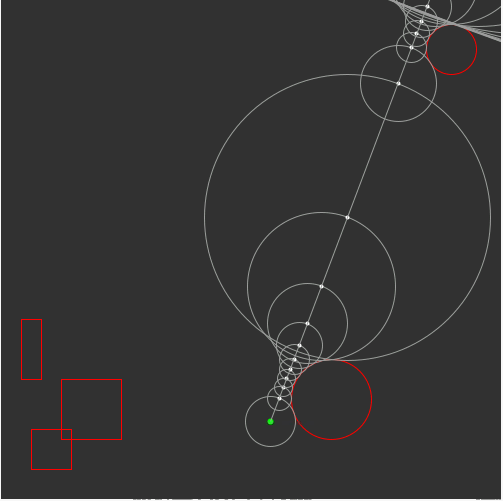
\includegraphics[width=8cm]{images/marching.png}
\begin{figure}[h]
    \centering
    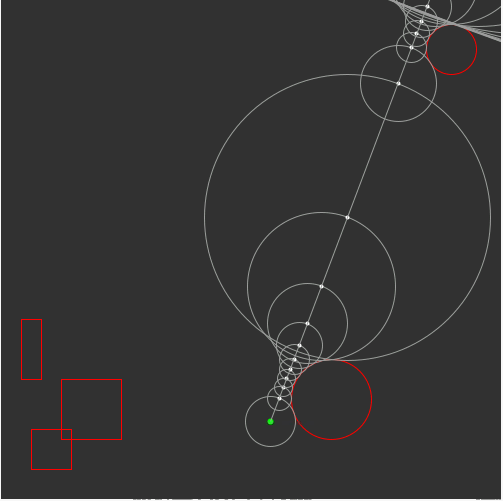
\includegraphics[width=8cm]{images/marching.png}
    \caption{Illustration 2D de la marche point par point d'un rayon (plus de details dans \ref{subsec:projection} \nameref{subsec:projection})}
    \label{fig:my_label}
\end{figure}

\clearpage
\documentclass[a4paper,11pt,twoside]{article} 
%\documentclass{article}

\input{charteINSA/maincharte.tex}

%\usepackage[french]{babel}

% resolve no citation problem
\nocite{*}
%\usepackage[...,backend=bibtex]{biblatex}

% Set page size and margins
% Replace `letterpaper' with `a4paper' for UK/EU standard size
%%%%%\usepackage[letterpaper,top=2cm,bottom=2cm,left=3cm,right=3cm,marginparwidth=1.75cm]{geometry}

% Useful packages
\usepackage{listings}

\input{preferences/listings-glsl.prf}
% optionally set GLSL as default language
\lstset{language=GLSL}
\input{preferences/glsl.tex}

\usepackage[square,numbers]{natbib}
\bibliographystyle{abbrvnat}
%Includes "References" in the table of contents
\usepackage[nottoc]{tocbibind}

\usepackage{setspace}
\usepackage{titletoc}
%\usepackage[T1]{fontenc}
%\usepackage{amsfonts}
%\usepackage{graphicx}
\usepackage{mathtools}
\graphicspath{ {images/} }

%\input{hautdepage.tex}
%\usepackage[colorlinks=true, allcolors=blue]{hyperref}


\begin{document}
\dosecttoc{} % generate TOC
%\maketitle
\clearpage

% Remerciements
\thispagestyle{empty} % removes page number
\subsection*{Remerciements}
Nous tenons à remercier notre tuteur de projet M. Sanchez, notamment pour son aide précieuse et ses conseils. \\
Nous remercions également Inigo Quilez pour la riche documentation sur le ray marching qu'il fournit librement sur son site web.
\clearpage

% TABLE DES MATIÈRES
\thispagestyle{empty} % removes page number
\setcounter{secnumdepth}{3}
\tableofcontents
\clearpage

\setcounter{page}{1}


\input{Parties/Introduction}
\clearpage
\input{Parties/Fonctionnement/main}
\clearpage
\input{Parties/Fonctionnalites/main}
\clearpage
\input{Parties/Historique/main}
\clearpage
\input{Parties/Conclusion}

\clearpage


%Imports the bibliography file "sample.bib"
\bibliography{sample}
\clearpage

% TABLE DES ANNEXES
\clearpage
\appendix
%\thispagestyle{empty} % removes page number
\sectionnn{Table des Annexes}
\addtocontents{toc}{\protect\setcounter{tocdepth}{0}}
\renewcommand{\stctitle}{}                          % Titre (issue with previous subsection showing up)
\renewcommand\thesubsection{A\arabic{subsection}}   % Numérotation
\renewcommand{\stcSSfont}{}                         % Police normale, pas en gras
\mtcsetrules{secttoc}{off}                          % Désactivation des lignes en haut et en bas de la table

% Affichage de la table des annexes
\secttoc
% ANNEXES
\clearpage
\pagenumbering{Roman}


\input{Parties/Annexes}

\mtcsetrules{secttoc}{off}

\end{document}


                        

\clearpage
\documentclass[a4paper,11pt,twoside]{article} 
%\documentclass{article}

\input{charteINSA/maincharte.tex}

%\usepackage[french]{babel}

% resolve no citation problem
\nocite{*}
%\usepackage[...,backend=bibtex]{biblatex}

% Set page size and margins
% Replace `letterpaper' with `a4paper' for UK/EU standard size
%%%%%\usepackage[letterpaper,top=2cm,bottom=2cm,left=3cm,right=3cm,marginparwidth=1.75cm]{geometry}

% Useful packages
\usepackage{listings}

\input{preferences/listings-glsl.prf}
% optionally set GLSL as default language
\lstset{language=GLSL}
\input{preferences/glsl.tex}

\usepackage[square,numbers]{natbib}
\bibliographystyle{abbrvnat}
%Includes "References" in the table of contents
\usepackage[nottoc]{tocbibind}

\usepackage{setspace}
\usepackage{titletoc}
%\usepackage[T1]{fontenc}
%\usepackage{amsfonts}
%\usepackage{graphicx}
\usepackage{mathtools}
\graphicspath{ {images/} }

%\input{hautdepage.tex}
%\usepackage[colorlinks=true, allcolors=blue]{hyperref}


\begin{document}
\dosecttoc{} % generate TOC
%\maketitle
\clearpage

% Remerciements
\thispagestyle{empty} % removes page number
\subsection*{Remerciements}
Nous tenons à remercier notre tuteur de projet M. Sanchez, notamment pour son aide précieuse et ses conseils. \\
Nous remercions également Inigo Quilez pour la riche documentation sur le ray marching qu'il fournit librement sur son site web.
\clearpage

% TABLE DES MATIÈRES
\thispagestyle{empty} % removes page number
\setcounter{secnumdepth}{3}
\tableofcontents
\clearpage

\setcounter{page}{1}


\input{Parties/Introduction}
\clearpage
\input{Parties/Fonctionnement/main}
\clearpage
\input{Parties/Fonctionnalites/main}
\clearpage
\input{Parties/Historique/main}
\clearpage
\input{Parties/Conclusion}

\clearpage


%Imports the bibliography file "sample.bib"
\bibliography{sample}
\clearpage

% TABLE DES ANNEXES
\clearpage
\appendix
%\thispagestyle{empty} % removes page number
\sectionnn{Table des Annexes}
\addtocontents{toc}{\protect\setcounter{tocdepth}{0}}
\renewcommand{\stctitle}{}                          % Titre (issue with previous subsection showing up)
\renewcommand\thesubsection{A\arabic{subsection}}   % Numérotation
\renewcommand{\stcSSfont}{}                         % Police normale, pas en gras
\mtcsetrules{secttoc}{off}                          % Désactivation des lignes en haut et en bas de la table

% Affichage de la table des annexes
\secttoc
% ANNEXES
\clearpage
\pagenumbering{Roman}


\input{Parties/Annexes}

\mtcsetrules{secttoc}{off}

\end{document}


                        

\clearpage
\documentclass[a4paper,11pt,twoside]{article} 
%\documentclass{article}

\input{charteINSA/maincharte.tex}

%\usepackage[french]{babel}

% resolve no citation problem
\nocite{*}
%\usepackage[...,backend=bibtex]{biblatex}

% Set page size and margins
% Replace `letterpaper' with `a4paper' for UK/EU standard size
%%%%%\usepackage[letterpaper,top=2cm,bottom=2cm,left=3cm,right=3cm,marginparwidth=1.75cm]{geometry}

% Useful packages
\usepackage{listings}

\input{preferences/listings-glsl.prf}
% optionally set GLSL as default language
\lstset{language=GLSL}
\input{preferences/glsl.tex}

\usepackage[square,numbers]{natbib}
\bibliographystyle{abbrvnat}
%Includes "References" in the table of contents
\usepackage[nottoc]{tocbibind}

\usepackage{setspace}
\usepackage{titletoc}
%\usepackage[T1]{fontenc}
%\usepackage{amsfonts}
%\usepackage{graphicx}
\usepackage{mathtools}
\graphicspath{ {images/} }

%\input{hautdepage.tex}
%\usepackage[colorlinks=true, allcolors=blue]{hyperref}


\begin{document}
\dosecttoc{} % generate TOC
%\maketitle
\clearpage

% Remerciements
\thispagestyle{empty} % removes page number
\subsection*{Remerciements}
Nous tenons à remercier notre tuteur de projet M. Sanchez, notamment pour son aide précieuse et ses conseils. \\
Nous remercions également Inigo Quilez pour la riche documentation sur le ray marching qu'il fournit librement sur son site web.
\clearpage

% TABLE DES MATIÈRES
\thispagestyle{empty} % removes page number
\setcounter{secnumdepth}{3}
\tableofcontents
\clearpage

\setcounter{page}{1}


\input{Parties/Introduction}
\clearpage
\input{Parties/Fonctionnement/main}
\clearpage
\input{Parties/Fonctionnalites/main}
\clearpage
\input{Parties/Historique/main}
\clearpage
\input{Parties/Conclusion}

\clearpage


%Imports the bibliography file "sample.bib"
\bibliography{sample}
\clearpage

% TABLE DES ANNEXES
\clearpage
\appendix
%\thispagestyle{empty} % removes page number
\sectionnn{Table des Annexes}
\addtocontents{toc}{\protect\setcounter{tocdepth}{0}}
\renewcommand{\stctitle}{}                          % Titre (issue with previous subsection showing up)
\renewcommand\thesubsection{A\arabic{subsection}}   % Numérotation
\renewcommand{\stcSSfont}{}                         % Police normale, pas en gras
\mtcsetrules{secttoc}{off}                          % Désactivation des lignes en haut et en bas de la table

% Affichage de la table des annexes
\secttoc
% ANNEXES
\clearpage
\pagenumbering{Roman}


\input{Parties/Annexes}

\mtcsetrules{secttoc}{off}

\end{document}


                        

\clearpage
\sectionnn{Conclusion}

Ce projet a été captivant et très motivant. Le fait de pouvoir observer rapidement les résultats de notre code était très agréable.\\
Nous avons rempli et même dépassé les objectifs que nous nous étions fixés.\\
Il était également intéressant de retrouver des notions vues en maths à l'INSA dans une application concrète.\\ \par

L'expérience fut très enrichissante car nous avons dû nous organiser pour pouvoir travailler en binôme sur le même code avec l'utilisation d'un gestionnaire de version (git) auquel nous nous sommes formés.\\
Nous avons pu explorer le principe du Ray Marching, découvrir un nouveau langage, le GLSL, ainsi que les bases de développement logiciel.\\ \par

Ce rapport était également l'occasion d'apprendre à maîtriser le LaTeX, mais c'était surtout l'occasion d'expliquer de façon claire et concise un concept technique.\\ \par

Finalement, ce projet de moteur graphique nous a beaucoup apporté et nous pensons continuer à le développer dans le futur.

\clearpage


%Imports the bibliography file "sample.bib"
\bibliography{sample}
\clearpage

% TABLE DES ANNEXES
\clearpage
\appendix
%\thispagestyle{empty} % removes page number
\sectionnn{Table des Annexes}
\addtocontents{toc}{\protect\setcounter{tocdepth}{0}}
\renewcommand{\stctitle}{}                          % Titre (issue with previous subsection showing up)
\renewcommand\thesubsection{A\arabic{subsection}}   % Numérotation
\renewcommand{\stcSSfont}{}                         % Police normale, pas en gras
\mtcsetrules{secttoc}{off}                          % Désactivation des lignes en haut et en bas de la table

% Affichage de la table des annexes
\secttoc
% ANNEXES
\clearpage
\pagenumbering{Roman}


\subsection{Scène simple}
%\addcontentsline{toc}{section}{Scène simple}
Code à mettre dans un fichier, nommé \emph{example.fs} par exemple
\begin{lstlisting}[language=GLSL]
#version 330 core
in vec2 FragCoord;
in float Time;
in vec2 MousePos;
in vec3 CamPos;
in vec3 CamDir;

out vec4 FragColor;
//uniform sampler2D generalTexture;

float SDF_Box_Frame( vec3 p, vec3 b, float e )
{
       p = abs(p  )-b;
  vec3 q = abs(p+e)-e;
  return min(min(
      length(max(vec3(p.x,q.y,q.z),0.0))+min(max(p.x,max(q.y,q.z)),0.0),
      length(max(vec3(q.x,p.y,q.z),0.0))+min(max(q.x,max(p.y,q.z)),0.0)),
      length(max(vec3(q.x,q.y,p.z),0.0))+min(max(q.x,max(q.y,p.z)),0.0));
}

float SDF_Circle(vec3 p,float r){
    return length(p)-r;
}

float SDF_Global(vec3 p){
    return min(
        SDF_Box_Frame(p,vec3(.5,.5,.5),0.1),
        SDF_Circle(mod(p+vec3(.5),vec3(1.,1.,1.))-vec3(.5),.15));
}

vec4 Get_Impact(vec3 origin,vec3 dir){//must have length(dir)==1 
    vec3 pos=origin;
    float dist;
    for(int i=0;i<30;i++){
        dist=SDF_Global(pos);
        pos+=dist*dir;
        if(dist<=.01) return vec4(pos,1.);
        if(dist>=20.0) return vec4(pos,-1.);
    }
    return vec4(pos,-1.);
}

vec3 grad(vec3 p){
    vec2 epsilon = vec2(.01,0.);
    return normalize(vec3(SDF_Global(p+epsilon.xyy)-SDF_Global(p-epsilon.xyy),
    SDF_Global(p+epsilon.yxy)-SDF_Global(p-epsilon.yxy),
    SDF_Global(p+epsilon.yyx)-SDF_Global(p-epsilon.yyx)));
}

vec3 Get_Color(vec3 origin,vec3 dir){
    vec4 impact = Get_Impact(origin,dir);
    if(impact.w<0.) return vec3(.5,.7,1.);
    vec3 normale=grad(impact.xyz);
    return normale;
}

void main()
{
    vec3 lookingAt = vec3(0.,0.,0.);
    vec3 posCam    = vec3(3.*sin(Time*.5),0.,3.*cos(Time*.5));
    
    vec3 ez = normalize(lookingAt - posCam); //base orthonormee
    vec3 ex = normalize(cross(ez,vec3(0.,1.,0.)));
    vec3 ey = cross(ex,ez);
    
    vec3 dir = normalize(FragCoord.x * ex + FragCoord.y*ey + 1.*ez);
    
  FragColor=vec4(Get_Color(posCam,dir),1.);
}
\end{lstlisting}

\mtcsetrules{secttoc}{off}

\end{document}


                        

\clearpage
\sectionnn{Conclusion}

Ce projet a été captivant et très motivant. Le fait de pouvoir observer rapidement les résultats de notre code était très agréable.\\
Nous avons rempli et même dépassé les objectifs que nous nous étions fixés.\\
Il était également intéressant de retrouver des notions vues en maths à l'INSA dans une application concrète.\\ \par

L'expérience fut très enrichissante car nous avons dû nous organiser pour pouvoir travailler en binôme sur le même code avec l'utilisation d'un gestionnaire de version (git) auquel nous nous sommes formés.\\
Nous avons pu explorer le principe du Ray Marching, découvrir un nouveau langage, le GLSL, ainsi que les bases de développement logiciel.\\ \par

Ce rapport était également l'occasion d'apprendre à maîtriser le LaTeX, mais c'était surtout l'occasion d'expliquer de façon claire et concise un concept technique.\\ \par

Finalement, ce projet de moteur graphique nous a beaucoup apporté et nous pensons continuer à le développer dans le futur.

\clearpage


%Imports the bibliography file "sample.bib"
\bibliography{sample}
\clearpage

% TABLE DES ANNEXES
\clearpage
\appendix
%\thispagestyle{empty} % removes page number
\sectionnn{Table des Annexes}
\addtocontents{toc}{\protect\setcounter{tocdepth}{0}}
\renewcommand{\stctitle}{}                          % Titre (issue with previous subsection showing up)
\renewcommand\thesubsection{A\arabic{subsection}}   % Numérotation
\renewcommand{\stcSSfont}{}                         % Police normale, pas en gras
\mtcsetrules{secttoc}{off}                          % Désactivation des lignes en haut et en bas de la table

% Affichage de la table des annexes
\secttoc
% ANNEXES
\clearpage
\pagenumbering{Roman}


\subsection{Scène simple}
%\addcontentsline{toc}{section}{Scène simple}
Code à mettre dans un fichier, nommé \emph{example.fs} par exemple
\begin{lstlisting}[language=GLSL]
#version 330 core
in vec2 FragCoord;
in float Time;
in vec2 MousePos;
in vec3 CamPos;
in vec3 CamDir;

out vec4 FragColor;
//uniform sampler2D generalTexture;

float SDF_Box_Frame( vec3 p, vec3 b, float e )
{
       p = abs(p  )-b;
  vec3 q = abs(p+e)-e;
  return min(min(
      length(max(vec3(p.x,q.y,q.z),0.0))+min(max(p.x,max(q.y,q.z)),0.0),
      length(max(vec3(q.x,p.y,q.z),0.0))+min(max(q.x,max(p.y,q.z)),0.0)),
      length(max(vec3(q.x,q.y,p.z),0.0))+min(max(q.x,max(q.y,p.z)),0.0));
}

float SDF_Circle(vec3 p,float r){
    return length(p)-r;
}

float SDF_Global(vec3 p){
    return min(
        SDF_Box_Frame(p,vec3(.5,.5,.5),0.1),
        SDF_Circle(mod(p+vec3(.5),vec3(1.,1.,1.))-vec3(.5),.15));
}

vec4 Get_Impact(vec3 origin,vec3 dir){//must have length(dir)==1 
    vec3 pos=origin;
    float dist;
    for(int i=0;i<30;i++){
        dist=SDF_Global(pos);
        pos+=dist*dir;
        if(dist<=.01) return vec4(pos,1.);
        if(dist>=20.0) return vec4(pos,-1.);
    }
    return vec4(pos,-1.);
}

vec3 grad(vec3 p){
    vec2 epsilon = vec2(.01,0.);
    return normalize(vec3(SDF_Global(p+epsilon.xyy)-SDF_Global(p-epsilon.xyy),
    SDF_Global(p+epsilon.yxy)-SDF_Global(p-epsilon.yxy),
    SDF_Global(p+epsilon.yyx)-SDF_Global(p-epsilon.yyx)));
}

vec3 Get_Color(vec3 origin,vec3 dir){
    vec4 impact = Get_Impact(origin,dir);
    if(impact.w<0.) return vec3(.5,.7,1.);
    vec3 normale=grad(impact.xyz);
    return normale;
}

void main()
{
    vec3 lookingAt = vec3(0.,0.,0.);
    vec3 posCam    = vec3(3.*sin(Time*.5),0.,3.*cos(Time*.5));
    
    vec3 ez = normalize(lookingAt - posCam); //base orthonormee
    vec3 ex = normalize(cross(ez,vec3(0.,1.,0.)));
    vec3 ey = cross(ex,ez);
    
    vec3 dir = normalize(FragCoord.x * ex + FragCoord.y*ey + 1.*ez);
    
  FragColor=vec4(Get_Color(posCam,dir),1.);
}
\end{lstlisting}

\mtcsetrules{secttoc}{off}

\end{document}


                        

\clearpage
\sectionnn{Conclusion}

Ce projet a été captivant et très motivant. Le fait de pouvoir observer rapidement les résultats de notre code était très agréable.\\
Nous avons rempli et même dépassé les objectifs que nous nous étions fixés.\\
Il était également intéressant de retrouver des notions vues en maths à l'INSA dans une application concrète.\\ \par

L'expérience fut très enrichissante car nous avons dû nous organiser pour pouvoir travailler en binôme sur le même code avec l'utilisation d'un gestionnaire de version (git) auquel nous nous sommes formés.\\
Nous avons pu explorer le principe du Ray Marching, découvrir un nouveau langage, le GLSL, ainsi que les bases de développement logiciel.\\ \par

Ce rapport était également l'occasion d'apprendre à maîtriser le LaTeX, mais c'était surtout l'occasion d'expliquer de façon claire et concise un concept technique.\\ \par

Finalement, ce projet de moteur graphique nous a beaucoup apporté et nous pensons continuer à le développer dans le futur.

\clearpage

%\addcontentsline{toc}{section}{Bibliography}
%\printbibliography

\sectionnn{Bibliographie}
Une biblio
\clearpage

% TABLE DES ANNEXES
\clearpage
\appendix
%\thispagestyle{empty} % removes page number
\sectionnn{Table des Annexes}
\addtocontents{toc}{\protect\setcounter{tocdepth}{0}}
\renewcommand{\stctitle}{}                          % Titre (issue with previous subsection showing up)

\renewcommand{\stcSSfont}{}                         % Police normale, pas en gras
\mtcsetrules{secttoc}{off}                          % Désactivation des lignes en haut et en bas de la table
\clearpage

% Affichage de la table des annexes
\secttoc

% ANNEXES
\clearpage
\pagenumbering{Roman}

\renewcommand\thesubsection{A\arabic{subsection}}   % Numérotation
\subsection{Scène simple}
%\addcontentsline{toc}{section}{Scène simple}
Code à mettre dans un fichier, nommé \emph{example.fs} par exemple
\begin{lstlisting}[language=GLSL]
#version 330 core
in vec2 FragCoord;
in float Time;
in vec2 MousePos;
in vec3 CamPos;
in vec3 CamDir;

out vec4 FragColor;
//uniform sampler2D generalTexture;

float SDF_Box_Frame( vec3 p, vec3 b, float e )
{
       p = abs(p  )-b;
  vec3 q = abs(p+e)-e;
  return min(min(
      length(max(vec3(p.x,q.y,q.z),0.0))+min(max(p.x,max(q.y,q.z)),0.0),
      length(max(vec3(q.x,p.y,q.z),0.0))+min(max(q.x,max(p.y,q.z)),0.0)),
      length(max(vec3(q.x,q.y,p.z),0.0))+min(max(q.x,max(q.y,p.z)),0.0));
}

float SDF_Circle(vec3 p,float r){
    return length(p)-r;
}

float SDF_Global(vec3 p){
    return min(
        SDF_Box_Frame(p,vec3(.5,.5,.5),0.1),
        SDF_Circle(mod(p+vec3(.5),vec3(1.,1.,1.))-vec3(.5),.15));
}

vec4 Get_Impact(vec3 origin,vec3 dir){//must have length(dir)==1 
    vec3 pos=origin;
    float dist;
    for(int i=0;i<30;i++){
        dist=SDF_Global(pos);
        pos+=dist*dir;
        if(dist<=.01) return vec4(pos,1.);
        if(dist>=20.0) return vec4(pos,-1.);
    }
    return vec4(pos,-1.);
}

vec3 grad(vec3 p){
    vec2 epsilon = vec2(.01,0.);
    return normalize(vec3(SDF_Global(p+epsilon.xyy)-SDF_Global(p-epsilon.xyy),
    SDF_Global(p+epsilon.yxy)-SDF_Global(p-epsilon.yxy),
    SDF_Global(p+epsilon.yyx)-SDF_Global(p-epsilon.yyx)));
}

vec3 Get_Color(vec3 origin,vec3 dir){
    vec4 impact = Get_Impact(origin,dir);
    if(impact.w<0.) return vec3(.5,.7,1.);
    vec3 normale=grad(impact.xyz);
    return normale;
}

void main()
{
    vec3 lookingAt = vec3(0.,0.,0.);
    vec3 posCam    = vec3(3.*sin(Time*.5),0.,3.*cos(Time*.5));
    
    vec3 ez = normalize(lookingAt - posCam); //base orthonormee
    vec3 ex = normalize(cross(ez,vec3(0.,1.,0.)));
    vec3 ey = cross(ex,ez);
    
    vec3 dir = normalize(FragCoord.x * ex + FragCoord.y*ey + 1.*ez);
    
  FragColor=vec4(Get_Color(posCam,dir),1.);
}
\end{lstlisting}


\mtcsetrules{secttoc}{off}


\end{document}


                        
